% !TeX encoding = UTF-8
% !TeX program = xelatex
% !TeX spellcheck = en_US

\documentclass[degree=master, degree-type=professional, language=chinese, fontset=none]{ustcthesis}
% degree      = doctor | master | bachelor
% degree-type = academic | professional | engineering
% language    = chinese | english
% fontset     = windows | mac | ubuntu | fandol

% 加载宏包、全部的配置
% !TeX root = ./main.tex

\ustcsetup{
  title              = {基于去噪扩散模型与3D高斯泼溅的水下三维感知增强方法及系统实现},
  title*             = {Underwater 3D Perception Enhancement Method and System Implementation Based on Denoising Diffusion Models and 3D Gaussian Splatting},
  author             = {鲍丙雷},
  author*            = {Bao Binglei},
  speciality         = {计算机技术},
  speciality*        = {Computer Technology},
  supervisor         = {阚震~教授, 于振中~研究员},
  supervisor*        = {Prof. Kan, Prof. Yu},
  % date               = {2025-3-6},  % 默认为今日
  % title              = {中国科学技术大学\\学位论文模板示例文档 v\ustcthesisversion},
  % title*             = {An example of thesis template for University of Science
  %                       and Technology of China v\ustcthesisversion},
  % author             = {李泽平},
  % author*            = {Li Zeping},
  % speciality         = {数学与应用数学},
  % speciality*        = {Mathematics and Applied Mathematics},
  % supervisor         = {XXX~教授, XXX~教授},
  % supervisor*        = {Prof. XXX, Prof. XXX},
  % date               = {2017-05-01},  % 默认为今日
  % professional-type  = {专业学位类型},
  % professional-type* = {Professional degree type},
  % department         = {数学科学学院},  % 院系,本科生需要填写
  % student-id         = {PB11001000},  % 学号,本科生需要填写
  % secret-level       = {秘密},     % 绝密|机密|秘密|控阅,注释本行则公开
  % secret-level*      = {Secret},  % Top secret | Highly secret | Secret
  % secret-year        = {10},      % 保密/控阅期限
  % reviewer           = true,      % 声明页显示“评审专家签名”
  %
  % 数学字体
  % math-style           = GB,  % 可选:GB, TeX, ISO
  math-font            = xits,  % 可选:stix, xits, libertinus
}


% 加载宏包

% 定理类环境宏包
\usepackage{amsthm}
\usepackage{amsmath}

% 插图
\usepackage{graphicx}

% 英文图题、表题
\usepackage{bicaption}

% 三线表
\usepackage{booktabs}

% 表注
\usepackage{threeparttable}

% 跨页表格
\usepackage{longtable}

% 算法
\usepackage[ruled,linesnumbered]{algorithm2e}
% \usepackage{algorighmic}

% SI 量和单位
\usepackage{siunitx}

\usepackage{adjustbox}


% 参考文献使用 BibTeX + natbib 宏包
% 顺序编码制
\usepackage[sort]{natbib}
\bibliographystyle{ustcthesis-numerical}

% 著者-出版年制
% \usepackage{natbib}
% \bibliographystyle{ustcthesis-authoryear}

% 本科生参考文献的著录格式
% \usepackage[sort]{natbib}
% \bibliographystyle{ustcthesis-bachelor}

% 参考文献使用 BibLaTeX 宏包
% \usepackage[style=ustcthesis-numeric]{biblatex}
% \usepackage[bibstyle=ustcthesis-numeric,citestyle=ustcthesis-inline]{biblatex}
% \usepackage[style=ustcthesis-authoryear]{biblatex}
% \usepackage[style=ustcthesis-bachelor]{biblatex}
% 声明 BibLaTeX 的数据库
% \addbibresource{bib/ustc.bib}

% 配置图片的默认目录
\graphicspath{{figures/}}

% 数学命令
\makeatletter
\newcommand\dif{%  % 微分符号
  \mathop{}\!%
  \ifustc@math@style@TeX
    d%
  \else
    \mathrm{d}%
  \fi
}
\makeatother
\newcommand\eu{{\symup{e}}}
\newcommand\iu{{\symup{i}}}

% 用于写文档的命令
\DeclareRobustCommand\cs[1]{\texttt{\char`\\#1}}
\DeclareRobustCommand\env[1]{\texttt{#1}}
\DeclareRobustCommand\pkg[1]{\textsf{#1}}
\DeclareRobustCommand\file[1]{\nolinkurl{#1}}

% hyperref 宏包在最后调用
\usepackage{hyperref}


% 手动设置字体
\setCJKmainfont{Songti SC}
% 如果上面不行,可以尝试:
% \setCJKmainfont{Source Han Serif SC Regular}  % 思源宋体

\begin{document}

\maketitle
\copyrightpage

\frontmatter
% % !TeX root = ../main.tex

\begin{innovations}

学术博士学位论文应当体现作者具有独立从事科学研究工作的能力,并在所学领域做出创造性的成果。
故在此须说明本学位论文的创新性,确保符合学术博士学位论文的创新要求,字数在800字以内。

\end{innovations}


% \begin{innovations}
%
% 工程博士学位论文应主要聚焦工程实践和应用研究,须体现工程性、创新性、实践性、应用性特征,
% 体现学位申请人在专业领域掌握坚实全面的基础理论和系统深入的专门知识,
% 具有独立承担专业实践工作的能力,在专业实践领域做出创新性成果,
% 对推动本专业领域知识和技术的发展作出重要贡献。
%
% 故在此须说明本学位论文的创新性及应用性,确保符合工程博士学位论文要求,字数在800字以内。
%
% \end{innovations}
  % 博士学位论文的创新性说明
% !TeX root = ../main.tex

\ustcsetup{
  keywords  = {水下三维感知, 去噪扩散模型, 3D 高斯泼溅},
  keywords* = {underwater perceptual, denoising diffusion models, 3D Gaussian splatting},
}

\begin{abstract}
  视觉感知是进行各种海洋勘探任务的重要手段,但是由于水介质对不同波长的光存在明显的吸收差异,尤其是对红光的吸收较为显著,导致水下图像常呈现出偏绿色调。同时,水下环境中的悬浮颗粒会在光线传播中产生散射,使得图像出现模糊,严重影响水下成像质量,恶劣的水下图像对各种水下任务如海洋环境观测、海洋工程项目维修、海洋资源探测以及海底遗迹测绘等带来困扰。
  因此,增强水下作业潜水员高质量全方位的辅助感知能力成为当前海洋科学领域亟需解决的问题。

  近年来,去噪扩散概率模型和3D高斯泼溅技术在图像生成和三维重建领域取得了显著的进展。
  本文以这两种技术为基础,提出一种基于去噪扩散模型的水下图像增强算法与水下高质量三维场景重建方法,
  并结合水下可穿戴式设备,设计了一种水下三维感知增强系统,旨在为潜水员提供一个可以自由控制视角的三维场景预览,
  潜水员可以利用该系统在潜水过程中查看目标物体的三维信息,从而辅助潜水员进行水下任务。本文具体研究内容如下:

  (1)考虑水下图像存在的严重退化问题,本文提出一种基于去噪扩散模型的水下图像增强算法。
  为了缓解扩散模型训练数据的规模依赖问题以及突破模型输出的尺寸限制,本文提出了基于补丁引导的去噪扩散模型采样过程。
  针对不同分辨率图像输入按照统一大小的补丁对图像进行分解,通过分解后的图像补丁级语义内容预测图像局部区域的噪声,
  将分解后的预测结果进行重新组合形成完整图像的噪声水平,进而采样出每个去噪阶段的完整图像语义信息与重建特征,
  让模型可以对任意分辨率的图像进行处理并生成相同尺寸的输出图像,同时缓解扩散模型训练数据的规模依赖。
  
  (2)本文提出一种基于3D高斯泼溅的水下目标场景高质量重建方法,
  首先将3D高斯在时间维度上进行水下动态场景的建模,结合高效的时空编码器与多头解码器进行3D高斯的时空变形预测,实现水下动态场景的初步重建。
  然后,本文受水流和光照影响的水下动态环境变换存在一个高频分布表示的启发,利用设计的场景过滤模块对学习到的动态重建场景信息进行低频场景数据的过滤,保留水下无扰动的目标场景信息,
  结合三阶段的自对抗训练模式适应水下环境的动态变换,消除水下运动干扰,更好的优化水下场景的高质量静态模式渲染。

  (3)基于上述两种算法,本文设计了一种水下可穿戴式三维感知增强系统。基于虚拟显示技术,本文搭建了一套可适用于水下环境中的可穿戴式系统,
  并结合预训练的水下3D高斯模型为潜水员提供一个可以自由控制视角的三维场景预览画面,
  同时提出一种基于手势识别的人机交互方法,潜水员可以利用手势控制视角的移动,从而获取目标物体的三维信息,辅助潜水员进行水下任务。

  % (1)通过研究去噪扩散模型的图像生成过程,结合水下图像衰减原理,探索利用去噪扩散模型进行水下图像增强的新颖方法,充分发挥扩散模型图像编辑能力恢复图像原始对比度和色彩,减轻由于水下恶劣环境对成像结果带来的语义干扰,为水下更多基于语义的下游任务提供高质量的图像输入基础。

  % (2)为了解决端到端的模型结构对于输入输入尺寸的限制,本文提出一种基于补丁引导的去噪扩散模型采样过程,针对不同分辨率图像输入可以按照统一大小的补丁对图像进行有重叠的分解,通过分解后的图像补丁级语义内容预测图像局部区域的噪声,将分解后的预测结果进行重新组合形成完整图像的噪声水平,进而采样出每个去噪阶段的完整图像语义信息与重建特征,实现任意分辨率的图像生成,同时缓解扩散模型训练数据的规模依赖。

  % (3)基于提出的水下图像增强方法,提出一种3D高斯泼溅技术在水下动态场景中的高质量重建方法。本文通过基于科尔莫格罗夫-阿诺德网络设计的高斯时空编码器与多头解码器进行水下动态场景重建。另外本文受水流和光照影响的水下动态环境变换存在一个高频分布表示的启发,利用学习到的动态重建场景信息进行低频视角数据的过滤,从而能够自适应水下环境的动态变换,消除水下运动干扰,更好的优化水下场景的高质量静态模式渲染。
\end{abstract}

\begin{abstract*}
  Underwater image enhancement technology is crucial for advancing marine research and exploration tasks. However, due to the significant absorption differences of light at different wavelengths in water, particularly the strong absorption of red light, underwater images often exhibit a greenish tint. Additionally, suspended particles in the underwater environment cause scattering during light propagation, resulting in image blurring, which severely affects the quality of underwater imaging. This issue poses challenges for various underwater tasks, such as marine environment monitoring, marine engineering maintenance, marine resource exploration, and underwater archaeology. Therefore, providing high-quality, reliable, and comprehensive sensory enhancement for underwater operations is an urgent issue in the field of marine science.

  In recent years, denoising diffusion models and 3D Gaussian splashing techniques have made significant progress in image generation and 3D reconstruction. This paper proposes an underwater image enhancement and high-quality 3D reconstruction method based on denoising diffusion models and 3D Gaussian splashing. The goal is to improve underwater image quality and enhance the accuracy of 3D scene reconstruction. The specific contributions of this paper are as follows:
	1.	Underwater Image Enhancement using Denoising Diffusion Models: Considering the severe degradation of underwater images, we propose an underwater image enhancement algorithm based on denoising diffusion models. By studying the image generation process of denoising diffusion models and combining the attenuation principles of underwater images, we explore a novel method for enhancing underwater images using diffusion models. This approach leverages the image editing capabilities of diffusion models to restore the original contrast and color of the images, alleviating semantic interference caused by the harsh underwater environment, and providing high-quality image input for downstream tasks based on semantic understanding.
	2.	Patch-guided Denoising Diffusion Sampling: To address the limitations of end-to-end model structures regarding input size, we propose a patch-guided denoising diffusion model sampling process. This method divides images of varying resolutions into overlapping patches of uniform size and predicts the noise of local regions based on the semantic content of these patches. The predicted noise results from the patches are then recombined to form the noise level of the complete image, allowing for the generation of images at arbitrary resolutions and alleviating the dependency on large-scale training data for diffusion models.
	3.	3D Gaussian Splashing for Dynamic Underwater Scene Reconstruction: Building upon the proposed underwater image enhancement method, we introduce a 3D Gaussian splashing technique for high-quality reconstruction of dynamic underwater scenes. We employ a Gaussian spatiotemporal encoder and multi-head decoder, designed based on the Kolmogorov-Arnold network, to reconstruct dynamic underwater scenes. Inspired by the high-frequency distribution representation caused by water flow and lighting changes, we filter low-frequency viewpoint data using learned dynamic reconstruction scene information, enabling adaptive changes to the underwater environment. This process eliminates motion interference and optimizes high-quality static scene rendering in underwater settings.

  This paper thus provides a comprehensive solution for enhancing underwater image quality and improving the accuracy of 3D scene reconstruction in dynamic underwater environments.
\end{abstract*}

\tableofcontents
% \listoffigures
% \listoftables
\listoffiguresandtables
% \include{chapters/notation}

\mainmatter
% !TeX root = ../main.tex

\chapter{绪论}

\section{研究背景与意义}
党的二十大报告指出:发展海洋经济,保护海洋环境,加快建设海洋强国。近年来,随着社会经济的不断发展,人类的生产活动对于各种资源如石油、土地、天然气以及生物资源的需求也不断增加,陆地资源的不断减少使得人们将注意力转移至海洋资源。
海洋蕴藏着丰富多样的生物和矿产资源 \cite{ocean_energy},与陆地相比,人类对于海洋资源的开发仍处于探索阶段。
随着各种海洋研究和勘探作业如水下观测、海底电缆或管道维护、水下考古遗址测绘和重建等任务的发展,
使得水下自主导航需求不断增加,自主潜水器(Autonomous Underwater Vehicle, AUV)和遥控潜水器(Remotely Operated Vehicle, ROV)己逐渐被应用在海上作业中 \cite{auv}\cite{rov}。
有些需要极高灵巧操作的水下任务还需要依靠人工完成,一些水下可穿戴设备可以在人类进行水下活动时提供必要的帮助 \cite{Xia2022},例如柔性外骨骼可以为髋关节内收提供辅助扭矩来增强人类水下活动 \cite{Xia2023}。
除了实现运动增强之外,水下图像也是认知水下信息的重要手段之一,在海洋勘探领域中一直占据着重要地位。\cite{underwater_perception}
AUV、ROV等水下机器人通过在设备终端配置水下相机来采集水下图像、视频数据,常常用于协助人类执行海洋勘探任务,采集到的数据将会被应用下水下科研领域,进而推动人类对海洋环境的探索与认知,因此高质量的水下图像对促进海洋勘探的发展意义重大。

然而,恶劣的水下环境给水下成像带来了一定的问题:一方面,水作为介质会不同程度地吸收不同波长的光,导致水下图像的色彩失真;另一方面,水中的悬浮颗粒会使水下光线产生轻微的角度偏转,导致图像的细节模糊。

失真的水下图像不仅会使观察者获得欠佳的视觉体验,还会对AUV、ROV等水下机器人上所搭载的视觉系统的正常运行产生严重干扰。
为了应对水下图像因光照匮乏而产生的问题,水下视觉系统常常会配备人工照明光源。然而,人工照明光源往往存在非均匀性的特点,这致使水下图像呈现出中间区域亮度偏高,整幅图像的亮度分布不均衡的状况,进而对成像的品质造成影响。
此外,鉴于水下成像环境的复杂性,水下成像系统难以从根源上消除由光散射所引发的图像模糊以及噪声的不良影响,所以仅仅依赖先进的成像设备是远远无法满足需求的。

伴随计算机技术的迅猛进步,数字图像处理技术取得了显著的发展,逐渐走向成熟,并且在众多领域(诸如医学、军事、监控、遥感等)均发挥着关键作用。
相较于提升成像系统设备性能所需的高昂成本,数字图像处理的方式更为灵活便捷,易于实施。
因此众多研究人员专注于运用数字图像处理技术来优化水下图像的视觉效果,提高成像质量,
水下图像处理技术也日益受到工业届和学术界的重视,越来越多的图像增强算法映入眼帘,在改善水下图像成像质量方面有着重要的应用,也可以便于后续水下识别、分割等任务的展开,极大地推动了海洋开发与勘探的发展。

由于在各类水下环境中光所遭受的衰减与散射程度不尽相同,尽管水下图像普遍展现出亮度较低、细节模糊的特征,然而在偏色状况以及模糊程度上,不同环境下的图像依然存在差别,因而难以进行统一的处理操作,这一情况为水下图像增强算法的研究增添了极大的困难。
当前,具备良好鲁棒性且切实有效的水下图像增强算法数量极为有限,多数算法仅仅能够针对单一或少数几种水体环境来实施图像增强处理,无法应对复杂多变且种类繁多的水体环境,这在很大程度上制约了这些算法的实际应用范围。
而且目前的图像增强算法对于所处理的图像分辨率大小也有所限制,特别是对于高分辨率的原始图像输入来说,许多算法需要重新设计,这给算法的实际应用带来了困难;
因此依靠图像处理算法鲁棒且稳定地增强水下图像仍是一个极具挑战性的任务。

另外,在需要人亲自参与的水下作业任务中,如何以一种有效的方式将对采集的视觉图像进行处理并反馈给潜水员,从而提高潜水员在水下的感知能力,也是需要解决的问题。\cite{underwater_perception}
基于虚拟现实的可穿戴设备是一种具有广阔前景的实现方式,将处理好的场景信息以三维可视化的途径呈现给潜水员,将有效提升潜水员在水下的感知能力。
目前主流的水下场景重建包括两个方向,一是以深度传感器如声纳为基础的水下稀疏或稠密点云的构建,另一个方向是基于视觉图像的水下三维重建研究,
其中基于新视角生成的逼真场景重建具有更强的适用性,尤其是对水下人体穿戴式设备来说,可以自然地实时渲染出媲美现实中的画面。
但是由于水下环境中存在的图像退化以及水流带来的场景动态扰动,使得水下环境除了采集的图像质量差外,也难以保持一个完全静态的场景,
实际进行新视角生成时要考虑场景的动态影响,包括水流带来的运动变化和光照不均匀带来的颜色变化,但是目前没有真正针对水下这种特殊场景进行去除扰动的重建研究。

综上所述,针对环境多变、条件恶劣的水下环境现状与实际场景需求,目前亟待解决的问题如下:

(1)水下图像增强算法局限大:大多数图像增强算法对于水下图像来说缺乏适应性,一些去雨、去雾建模中忽略的因素在水下图像增强问题中需要重新考虑,比如水陆环境不同透射率的影响。
采用更强大的复杂模型或框架在一定程度上可以提升模型的泛化能力,但是需要足够多的高质量数据集来支撑。
与去雨、去雾问题相比,水下图像增强问题不仅在真实环境下获得水下退化和清晰的成对图像难度巨大,且采用合成数据的方式获取成对图像数据集也极为困难,
现有的依靠物理模型合成水下图像数据集的方式,往往通过简化模型来生成有色偏和雾效应的图片,并不能精确描述水下环境。
另外,许多模型往往是针对固定的图像分辨率进行训练,高分辨率的图像输入往往需要重新设计模型,这给模型的实际应用带来了困难。

(2)水下三维建模能力弱:劣质的水下环境会对图像的语义信息带来干扰,这让一些依赖图像语义的下游任务带来挑战。在三维重建的前期数据预处理阶段,
采用这种退化的水下图像进行相机位姿估计时,会因关键点匹配错误导致相机位姿估计结果不准确,从而影响点云生成结果。
另外由于水流造成的动态扰动,会使得不同时刻的场景发生轻微变化,这导致最终的渲染时场景中的某些位置会出现模糊,影响视觉效果,
而加入时间信息进行时空建模时又需要考虑由于模型复杂度提升带来的推理成本问题,影响原本的渲染效率。

(3)缺乏行之有效的感知增强系统:对于复杂的水下任务如事故救援打捞,水下勘探等情况,人类的灵巧操作难易被水下机器人取代,而人在水下环境中的各视觉感官被严重虚弱,
通过在人体水下可穿戴设备上集成感知增强功能可以辅助潜水员在水下环境中的工作,但是目前很少有类似的系统能够将水下环境信息以一种直观、清晰的方式呈现给潜水员。
同时可靠的人机交互也是提升潜水员在使用水下设备时体验的关键,复杂的交互指令往往需要潜水员花费大量的时间学习,这会降低潜水员在水下作业的效率,
亟须一种自然、直观的交互方式提高潜水员在使用系统时的体验。

% (1)模型局限性大
% 与去雨、去雾问题相比,水下图像的建模更为复杂也更为精细。去雨、去雾建模中忽略的一些因素和近似的一些参数,在水下图像增强问题中需要重新考虑,比如水陆环境不同对透射率的影响。除了复杂的水下图像建模过程,传统方法增强水下图像会采用若干已知先验来加强模型对水下环境的刻画,涉及到调整各个约束项之间权重大小,需要人工协调,时间代价昂贵。基于先验的增强方法的优劣程度取决于模型对真实环境的刻画是否完善,对于繁多复杂的水下环境的适应性是否优良,采用的约束是否精确,但是这需要对任务深刻的理解和高超的数学建模技巧以及大量的时间。

% (2)数据获取难度大
% 基于深度学习的水下图像增强方法依赖大量的数据,解决越复杂的问题,网络需要越大的参数量。数据量越大,深度模型鲁棒性越好。同样与去雨、去雾问题相比, 水下图像增强问题不光在真实环境下获得水下图像和清晰的图像难度巨大,采用合成数据的方式获取图像对数据集也极为困难。现有的依靠物理模型合成水下图像数据集的方式,往往通过简化模型来生成有色偏和雾效应的图片,并不能精确描述水下环境。 图像对采用的干净图像往往是陆上的干净图像,这与水下环境并不类似。因此,图像对数据集的缺失为水下图像增强问题的解决带来了困难。

% (3)泛化能力弱
% 目前基于深度学习的水下图像增强算法仍依赖于指定的训练测试集,对于复杂多变的真实场景的水下图像,即训练集尚未包括的水下环境类型,图像增强的结果并不能让人满意,如何扩展数据集,适配多种复杂环境下的水下图像成为水下图像增强算法和实际应用中的巨大挑战。

本文将从水下图像增强问题出发,结合水下场景需求,提出一种基于去噪扩散模型与3D高斯泼溅的水下三维感知增强系统,
通过将采集到的原始数据通过图像增强算法生成高质量的水下图像,并利用3D高斯泼溅模块得到优化后的三维可视化模型,
最后借助可穿戴设备和手势交互指令为潜水员提供更加直观、清晰的水下环境信息,从而提高水下作业的效率。


\section{国内外研究与发展现状}
\subsection{水下图像增强技术国内外现状}
目前水下图像增强技术大致可以分为以下三类:基于物理模型的方法、基于先验知识的方法和基于深度学习的方法。
\subsubsection{基于物理模型的方法}
基于物理模型的方法依赖于水下图像生成过程的数学模型来增强水下图像 \cite{uw_img_math1}\cite{uw_img_math2}:
\begin{equation}
I=J \cdot e^{-\beta d}+B^{\infty} \cdot\left(1-e^{-\beta d}\right),
\label{IFM1}
\end{equation}
其中$I$是水下退化后的图像,$J$是未衰减的图像,$B^{\infty}$是大气光照, $\beta$是衰减系数,$d$是相机到物体的距离。
该模型与陆地图像恢复方法中常用的图像生成过程模型类似 \cite{ifm},用数学模型从退化原理出发表示了水下图像的衰减与散射过程。
2018年,Akkaynak等人\cite{modified_uw_img_math}通过使用$\beta^D\left(\mathbf{v}_D\right)$和$\beta^B\left(\mathbf{v}_B\right)$修正其中的前向衰减系数和后向衰减系数更新了水下图像生成数学模型:
% \begin{equation}
% I_c=J_c e^{-\beta_c^D\left(\mathbf{v}_D\right) \cdot z}+B_c^{\infty}\left(1-e^{-\beta_c^B\left(\mathbf{v}_B\right) \cdot z}\right)
% \label{IFM2}
% \end{equation}
\begin{equation}
    I=J e^{-\beta^D\left(\mathbf{v}_D\right) \cdot d}+B^{\infty}\left(1-e^{-\beta^B\left(\mathbf{v}_B\right) \cdot d}\right).
    \label{IFM2}
\end{equation}

还有一些利用其他辅助信息进行图像恢复的方法,如基于深度图\cite{depth_img}、连续的多帧图像\cite{multi_frame}和偏振图像\cite{U2PNet}等信息的水下图像增强算法。
这些方法可以更好的估计水下图像生成模型中的参数并获得清晰的图像。
多源传感器的信息融合技术\cite{fusion}可以依靠语义补充来提升水下图像增强的表现,然而它们通常需要特定的硬件支持,如 RGBD 相机和偏振相机。
总的来说,基于物理模型的方法系统地描述了水下图像的生成过程,并为水下图像增强提供了一个参考模型,对水下图像增强任务具有一定的理论指导作用,
但是假设的模型在适应复杂多样的水下环境方面仍然面临挑战,准确估计多个参数仍然是一项具有挑战性的工作。

\subsubsection{基于先验知识的方法}
基于先验知识的水下图像增强方法主要是利用从图像亮度、颜色、对比度等因素总结出的统计学规律来恢复图像质量。
与物理模型方法相比,这类方法通常不需要额外设备支持,仅通过对单张图像的处理即可达到增强效果,因此在实际应用中具有更强的灵活性。
根据先验知识的不同级别可以将基于先验知识的水下图像增强方法分为传统图像处理方法和高级统计推断方法两大类。

第一种方法涉及应用传统的图像处理技术,根据常规的先验知识将图像亮度和饱和度等图像属性恢复到正常水平,例如:直方图均衡(Histogram Equalization, HE)\cite{he}、对比度限制自适应直方图均衡(Contrast Limited Adaptive Histogram Equalization, CLAHE)\cite{clahe}、伽马校正和广义反锐化掩蔽 (Generalized Unsharp Masking, GUM) \cite{gum},
这类方法不考虑水下图像的成像过程,直接通过直方图拉伸或线性变换等方法对颜色模型中的像素进行修改,以扩展图像的动态像素范围,提高图像对比度并缓解图像色偏问题。
2013 年,Hitam 等人\cite{mixture_clahe}提出一种专门适用于水下图像增强的 CLAHE 方法, 他们在由色调、 饱和度和明度构成的色彩空间(Hue Saturation Lightness, HSL)和由红色、绿色和蓝色构成的色彩空间(Red Green Blue, RGB)上进行 CLAHE 运算,并使用欧几里德范数将两个结果组合在一起,有效提高了水下图像的对比度,并降低了图像中的噪声和伪影。
Retinex 是一种基于颜色恒常性理论的经典图像增强方法,
2014 年,Fu 等人\cite{uw_retinex}提出基于 Retinex 模型的水下图像增强方法,采用了 Retinex 的水下图像处理变分框架,他们从水下退化图像中分解出反射分量和照明分量,可以有效恢复图像亮度和校正图像色彩。
但这些方法都缺乏系统指导,不具备很强的泛化能力。

基于高级统计推断的先验方法通过统计正常图像中的潜在规律来估计水下图像生成模型中的相关基本参数,从而实现图像质量提升。
这些方法源于特定环境下的图像先验知识,在多种场景中具备一定的泛化能力。
何等人 \cite{dcp} 通过观察大量无雾图像的暗通道图数据,发现正常无雾图像的暗通道几乎为零,于是提出了一种名为暗通道先验(Dark Channel Prior, DCP)的图像去雾算法,在图像去雾任务中取得了令人惊叹的结果。
受到暗通道先验算法在陆地天气去雾为主的一系列任务中取得成功的启发,2013 年,Drews 等人 \cite{udcp}对传统的暗通道先验算法进行了水下的改进,提出一个新的仅考虑绿色和蓝色通道的水下暗通道先验方法(Underwater Dark Channel Prior, UDCP),更加符合水下环境中短波红色光被严重衰减的背景。
然而,由于水下环境复杂,统计出的先验知识可能在某些情况下失效,导致形如DCP这一类的方法在水下可能会表现出亮度或者色彩恢复的不稳定性,甚至在一些极端的水下环境中出现失真或细节丢失的问题。

\subsubsection{基于深度学习的方法}
与传统的基于物理模型和先验知识进行水下图像增强的方法不同,基于深度学习的方法可以基于神经网络从大规模成对数据中学习到图像特征和潜在的非线性映射关系。
神经网络模型通过构建复杂的网络结构,可以有效地捕捉图像中的低光、噪声、色彩偏移等特性,并在增强过程中实现对图像细节的高保真还原。
因此,深度学习方法在处理复杂的水下图像时展现出强大的适应性和鲁棒性。
经典的深度学习方法往往以有监督学习的方式,经过多次的卷积和反置卷积操作进行特征提取和恢复来重建清晰的图像。
这些方法在图像处理领域已经展现了显著效果,如在图像超分辨率\cite{cyberCSRnet}、图像去雾\cite{QCNN_H}、曝光校正\cite{Exposure_restoration}和语义重建\cite{InpaintingMissingArea}等任务中都涌现出许多优秀的算法。
有监督的深度学习方法旨在通过对应的特征解码器和编码器以数据驱动的方式学习权重来恢复水下图像,即算法需要用包含原始水下图像和其对应理想参考图像的数据集来进行训练和评估。
2020 年,Anwar 等人 \cite{uwcnn}提出了 UWCNN 水下图像增强算法,他们引入了一种专门用于水下场景图像增强的卷积神经网络(Convolutional Neural Network, CNN)模型,并且使用从现实世界陆地图像生成的各种合成水下风格图像来训练模型学习图像的恢复模式,
然而,由于训练数据的合成性质,这种方法在模型的泛化性上表现不佳。

由于水下理想参考图像获取困难,研究人员很难同时获取真实的水下场景和其相应的理想参考图像,因此现有深度学习增强方法多流行使用基于生成对抗网络(Generative Adversarial Network, GAN) \cite{gan}的方法避免对参考图像的依赖。
GAN 通过生成器和判别器之间的对抗训练,可以生成更真实且无噪声的水下图像。
2018 年, Li 等人 \cite{water_gan}提出了 WaterGAN 方法,该方法以 RGB 图像以及对应的深度图分别作为输入,从而将网络分为水下图像合成和颜色恢复两个部分,图像合成部分用于输出合成水下图像,颜色恢复部分将未经标记的水下图像作为输入,输出恢复后的图像及对应深度图。
同年,Fabbri 等人 \cite{ugan}提出 UGAN,该方法只需输入单张图像,不需要深度图等额外信息的输入,实现了对水下彩色图像的有效增强。
2019 年, Chen 等人 \cite{gan-rs}提出的 GAN-RS 利用多个判别器来引导生成器抑制水下噪声,多个鉴别器可以让GAN-RS 进一步增强生成器生成更真实且无噪声的水下图像的能力。
2020 年,Islam 等人 \cite{funie_gan}提出了一个快速水下图像增强算法 FUnIE-GAN,并将其应用到了水下机器人的目标检测以及人类姿势检测任务中。作者还利用 CycleGAN \cite{cycle_gan}生成了一个名为 EUVP(Enhanced UnderwaterVision Dataset)的大型水下数据集,其中包含数万张已配对的水下图像。
2021 年,Zhu 等人 \cite{dehaze_gan}提出了 DehazeGAN,这是一种利用多尺度生成器来预测水下图像生成模型中的大气光和传输图的方法,实现通过结合 GAN 与 水下图像物理生成模型来恢复水下图像。
但由于GAN无法控制生成样本的模式,训练过程经常会遇到收敛困难等问题,同时由于水下场景的复杂性和多样性,基于预训练的 GAN 模型在对不同数据集进行迁移微调时容易发生训练不稳定与崩溃现象,
因此基于 GAN 的水下图像增强方法在鲁棒性和泛化方面表现依旧不够理想。

与 GAN 相比,去噪扩散概率模型 \cite{pre_ddpm}\cite{ddpm}是一种基于概率似然的模型,且在近年来已经证明了其具有生成高质量图像的能力。
去噪扩散模型以其简单性和可扩展性而闻名,该模型可以从简单的初始噪声分布中逐步生成逼真且高质量的图像,在许多任务中展现出超越GAN的结果,这使其对包括水下图像增强在内的各种图像生成任务具有吸引力。
2021 年,OpenAI 的研究人员通过实验证明扩散模型相比 GAN 在大多数任务中可以表现的更好,并且他们提出了一种由分类器引导的扩散训练方法\cite{ddpm_beat_gan},确保生成的样本保持其真实性并与目标样本分布保持一致。

然而,去噪扩散模型需要经过大约上千个去噪步骤来生成最终的结果,这导致其推理速度较为缓慢,特别是在生成高分辨率图像时需要很长的时间。
2022 年,Rombach 等人 \cite{latent}借助自动编码器,提出一种在图像潜在空间进行扩散训练的方法,以在降低复杂性和保持图像细节之间实现近乎最优的权衡。
另一种加速扩散模型推理时间的方法是缩短扩散模型的反向采样步骤,如改进的隐式扩散方法 \cite{improved_ddpm,ddim}设计了一种新的采样器,可以用更少的时间步数进行去噪采样,从而加速扩散模型的推理过程。
通过利用这一改进,扩散模型中的采样过程变得更加高效,并且可以在预训练的扩散模型中直接使用,无需重新训练模型,有助于增强扩散模型在不同任务上的的整体性能和可扩展性。
2023年,Özdenizci 等人 \cite{weather}利用条件扩散模型在恢复恶劣天气条件下的图像研究中取得了卓越效果,他们提出了一种基于补丁的方法来恢复不同尺寸的图像。
然而,他们将图像分辨率统一为 16 的倍数,以便于获得补丁,但这仍然引入了图像在像素空间的重新调整,导致图像生成过程中的像素细节丢失。

总的来说,基于目前去噪扩散模型在图像生成领域相比GAN表现出的优越性,可以看出去噪扩散模型在水下图像增强方面具有一定的潜力,尽管其生成时间较长,但可以利用在潜在空间采样或者借助隐式扩散采样的方式提升模型效率。

\subsection{水下三维重建技术国内外现状}
探索水下三维场景重建技术对于海洋工程、环境保护等具有重大意义。
近年来,国内外研究人员围绕该技术的关键问题展开了深入研究,主要集中于以下两个方向。

\subsubsection{传统三维点云重建方法}
传统三维点云重建的一种方法是基于深度传感器(如声纳、激光等)等设备,通过采集水下环境的稀疏或稠密点云实现三维建模 \cite{sonar1}\cite{sonar2},
深度传感器在水下环境中表现出较强的抗干扰能力,但受限于设备成本及数据处理复杂性,其应用仍面临较大挑战;
另外,基于计算机视觉的点云生成也是一种重要的水下三维重建方法,代表性技术包括SfM( Structure from Motion)\cite{sfm1, sfm2} 和Multi-view Stereo(MVS) \cite{mvs}。
SfM通过分析多视角图像的几何关系生成稀疏点云,而MVS则进一步利用多幅图像的视差信息进行三角测量,从而生成高精度的稠密点云。
这两种方法都需要对来自不同角度的图像进行特征提取和匹配,常用算法如SIFT \cite{sift} 和 ORB \cite{orb},在图像特征点对齐方面具有较高的可靠性。
并且近年来随着机器学习的引入,极大地提升了图像特征匹配的精度。
例如,2023年Lindenberger等人 \cite{lightglue} 提出了基于神经网络的图像特征匹配方法,该方法通过跨图像的局部特征学习,在提升匹配精度的同时,大幅降低了内存和计算需求。
2024年,Wang等人 \cite{enhancing-mvs} 引入了Twin-FPN架构,结合多尺度特征损失,在复杂的室内场景中实现了更高效的通用特征表示。

然而,传统三维重建方法在水下应用中受到诸多限制,传统的三维点云不利于潜水员直观的理解水下环境,单纯的点云数据无法观察水下物体的细节纹理,这对一些需要精细操作的场景,如水下管道维护、水下考古等场景来说,存在较大的局限性。


\subsubsection{基于图像的新视角生成}
基于视觉图像的水下三维重建除了可以形成场景的点云表示\cite{vision_recon} ,也可以通过新视角生成(Novel View Synthesis, NVS)技术渲染出更逼真的任意视角的新图像,
其更多应用在水下人体穿戴式设备中 \cite{Xia2023}\cite{underwater_perception},可以极大地增强用户的环境感知能力,推动水下虚拟现实技术的发展。
神经辐射场(Neural Radiance Fields, NeRF) \cite{nerf}\cite{Mip_nerf360} 是NVS领域中的一类代表性框架。
NeRF通过定义隐式函数来表征三维场景,并通过体积渲染 \cite{volume_render} 方法生成高质量的多视角图像。
然而,由于在光线行进路线上的频繁采样让NeRF具有高额的计算成本,限制了其在实时场景渲染中的应用。
为此,2022年提出的Instant NeRF \cite{instant_nerf} 通过多功能编码器显著降低了NeRF的训练成本,允许在几乎不牺牲质量的情况下利用较小的网络来大大减少浮点运算和内存访问次数。
此外,2023年Cao等人提出了HexPlane方法 \cite{hex_plane},通过高效的融合从不同二维平面中提取的向量来计算时空点的特征,在动态场景上将训练时间减少了100多倍。

与NeRF的隐式表示不同,3D高斯泼溅(3D Gaussian Splatting, 3DGS) \cite{3DGS} 提供了一种显式的场景表示方法,结合可微分的光栅化渲染,可以显著提升NVS的渲染速度与质量。
基于3D高斯的可变形扩展\cite{dynamic_3DGS1}\cite{dynamic_3DGS2}\cite{dynamic_3DGS_efficient}\cite{4DGS},还可以直观的完成动态场景的三维重建。
2024年,Guo等人\cite{flow_2024motion}为了更好的捕捉场景中的动态信息,通过在训练中增加光流损失对变形范式进行优化,建立了高斯运动和图像像素流之间的对应关系,提高了3DGS在动态场景建模时的质量。

综合以上对水下图像增强和三维重建技术的研究现状,可以看出去噪扩散模型和3D高斯泼溅技术在水下图像增强和三维重建任务中具有一定的潜力,但目前仍存在以下问题:

(1)水下图像增强方面,目前基于去噪扩散模型的系列方法在陆地图像增强方面已经取得了较好的效果,但其在水下图像增强方面的应用仍处于起步阶段,问题在于:
一是需要采用合理的策略解决水下图像数据集获取困难与扩散模型数据规模依赖之间的矛盾;
二是在实际应用中正确处理扩散模型推理速度差与生成能力强之间的矛盾。
% 角色定位

(2)水下三维重建方面,基于图像的新视角生成技术可以结合可穿戴设备提供给潜水员更直观的视觉感知,但目前还没有相关的研究将3DGS技术应用于水下三维重建,问题在于:
一是本身缺少水下三维重建数据集,模型有效性在水下难以得到有效验证;
二是如何在水下动态环境中消除运动干扰,同时保留原始3DGS的高效渲染能力。


\section{本文主要工作与组织结构}
\subsection{本文主要工作}
基于上述对水下图像增强任务以及三维重建工作的研究现状与问题分析,本文针对目前水下图像恢复难、水下三维感知质量差等问题,提出了基于去噪扩散模型以及3D高斯泼溅技术的水下图像增强以及三维重建方法,
% \cite{patch_based_ddpm}
并在此基础上结合水下可穿戴式平台设计一套有效的水下三维增强感知系统,用于辅助潜水员在进行水下作业时实时预览目标场景的三维信息。
\begin{figure}
    \centering
    \includegraphics[width=0.95\textwidth]{figures/ch1/overview.pdf}
    \caption{本文主要研究内容}
    \label{img:overview}
\end{figure}

本文的主要研究内容如图\ref{img:overview}所示,包括以下几个方面:

(1)本文提出一种基于补丁引导采样过程的去噪扩散模型方法,并结合补丁大小重新设计噪声估计网络结构,利用条件扩散模型实现水下图像的增强。
这种补丁级别的处理方式不仅缓解了扩散模型对数据规模的依赖,同时让提出的方法突破分辨率限制,适用于任意分辨率图像的处理。
同时,考虑扩散模型的推理速度与生成能力之间的矛盾,该算法的结果主要用来为接下来的三维重建提供高质量的多视角图像,而不用考虑其实时性差带来的担忧。
% \cite{patch_based_ddpm}

(2)本文提出一种基于3DGS的水下三维重建方法。结合4D动态高斯泼溅技术在动态场景重建中的能力,本文设计了一种多阶段的递进式训练模式,
通过筛选出原始数据集中的高频次目标场景,实现水下目标场景的高质量重建,从而保留原有3DGS的渲染速度,
并制作了专门的水下三维重建数据集,用于验证提出的方法在复杂水下环境中的重建效果。

(3)基于虚拟现实技术,本文搭建了一套可适用于水下作业的穿戴式平台,结合预训练的水下3D高斯模型为潜水员提供一个可以自由控制视角的三维场景预览画面,
同时提出一种基于手势识别的人机交互方法,潜水员可以利用手势控制预览画面中的视角,从而实现对水下场景的实时感知,具有较强的实用性和应用前景。
% \cite{underwater_perception}

% (1)技术前沿性:随着深度学习技术的发展,去噪扩散概率模型在图像生成领域逐步取代生成对抗网络的在许多任务中的应用,本文拟将去噪扩散概率模型和去噪扩散隐式模型应用于水下图像增强,该技术代表了图像生成领域的前沿发展,具有强大的图片编辑能力;同时,3D高斯泼溅技术在三维重建领域取得了显著的进展,本文拟将3D高斯泼溅技术应用于水下三维重建,该技术具有高效的渲染速度和质量,能够实现动态场景的实时表示。

% (2)创新处理策略:在水下图像增强方面,

% (3)系统完整性:本文将水下图像增强技术和水下三维重建技术相结合,设计一套完整的水下三维增强感知系统,该系统能够提高水下图像质量和三维场景重建精度,为水下作业提供辅助感知增强,具有较强的实用性和应用前景。

\subsection{本文组织结构}
第一章绪论:本章主要阐述了研究背景和意义,强调在海洋资源开发需求增长的背景下,水下图像和三维感知对于海洋勘探的重要性,以及当前水下环境成像面临的问题和挑战。同时,详细分析了水下图像增强和三维重建技术的国内外研究现状,明确了现有方法的不足,进而提出本文旨在解决水下图像恢复难、三维感知质量差等问题,通过基于去噪扩散模型和3D高斯泼溅的技术,设计水下三维感知增强系统,辅助潜水员水下作业。

第二章相关技术与理论:对支撑本研究的核心技术进行了系统介绍,包括去噪扩散概率模型、去噪扩散隐式模型、3D高斯泼溅技术,以及U-Net网络和Kolmogorov-Arnold网络。这些技术为后续章节中水下图像增强算法和三维重建框架的设计提供了坚实的理论基础。

第三章基于去噪扩散模型的水下图像增强算法:针对水下图像存在的语义衰减问题,提出了基于补丁引导的去噪扩散模型水下图像增强算法。该算法通过基于滑动窗口的补丁获取方式,将图像分解为固定大小的补丁,降低了模型对数据集规模的依赖,同时实现了对任意分辨率水下图像的增强。在采样过程中,利用条件扩散模型原理,将退化的水下图像作为条件信息引入,确保生成结果的保真度。此外,设计了专门的噪声估计网络,通过引入残差模块和注意力机制,提升了噪声预测的精度。通过在EUVP和UIEB数据集上的实验,与多种现有方法对比,验证了该方法在水下图像增强方面的有效性,在主观视觉效果和客观指标上均表现出色。

第四章基于3D高斯泼溅的水下三维重建:鉴于3D高斯泼溅技术在新视角生成领域的优势以及水下三维重建面临的挑战,如缺少专门数据集、图像退化和动态扰动等问题,提出了基于3D高斯泼溅和KAN变形机制的水下目标场景三维重建方法。通过设计3D高斯时空编码器和基于KAN的特征解码器,实现了对水下动态场景的4D时空建模优化,提高了重建的精度和稳定性。采用多阶段训练模式和场景过滤模块,有效抑制了运动干扰,提升了静态场景的重建质量。构建了水下重建数据集3DUW,并在该数据集和公开数据集SeaThru-NeRF上进行实验,结果表明该方法在水下场景重建的准确性和实时性方面具有显著优势。

第五章水下穿戴式感知增强系统设计:为提升潜水员在水下复杂环境中的感知能力,基于前文提出的水下图像增强算法和三维重建技术,设计了可穿戴式水下感知增强系统。在需求分析方面,明确了系统需具备水下视觉增强、实时三维渲染、可靠运行平台和自然人机交互等功能。通过可行性分析,从视觉增强功能完整性、系统实时性、可靠性和人机交互等角度论证了系统设计的可行性。在系统实现上,完成了硬件选型与系统架构搭建,包括相机、头戴式显示器、嵌入式处理器和电源模块等的选择和平台的防水与机械设计。同时,集成了图像增强与三维重建、用户交互与控制以及VR界面设计等功能,为潜水员提供了全面且清晰的水下环境信息,提升了水下作业效率。

第六章总结与展望:总结了全文的研究成果,回顾基于去噪扩散模型和3D高斯泼溅技术在水下图像增强和三维重建任务中的优势和创新点。同时,对未来的研究方向进行展望,指出当前研究存在的不足,如显示屏分辨率有待提高、功能可进一步扩展等,并提出了相应的改进方向和研究思路,为后续研究提供参考。 

% !TeX root = ../main.tex

\chapter{相关技术与理论}
本章系统阐述支撑本研究的三项核心技术与理论:去噪扩散概率模型、3D高斯泼溅(3D Gaussian Splatting, 3DGS)技术及相关深度学习基础。
三者通过协同作用构建了完整的水下感知增强体系:
首先,基于去噪扩散模型的水下图像增强算法(详见第三章)通过渐进式噪声去除机制恢复退化图像的语义信息;
其次,增强后的多视角图像经由3D高斯泼溅技术(详见第四章)构建动态场景的显式三维表征;
最终,通过可穿戴设备实现水下三维场景的实时渲染与交互,辅助潜水员进行水下作业。
另外,U-Net网络与Kolmogorov-Arnold(KAN)网络分别作为图像增强与三维重建的核心组件,
U-Net用于扩散模型的噪声估计,KAN网络用于3D高斯的时空形变预测。

% 本章重点介绍本文研究内容所涉及的去噪扩散概率模型、3D高斯泼溅技术以及相关深度学习的基本理论知识。
% 其中,去噪扩散模型作为本文水下图像增强的核心技术,用于修复和优化退化的水下图像质量;
% 利用经过增强的水下某个场景的多视角图像,结合3D高斯泼溅技术,可实现水下三维场景的高质量重建,
% 三维渲染图像可以通过可穿戴设备展示给潜水员,从而辅助潜水员进行水下作业。
% 另外,在去噪扩散模型中将利用U-Net网络作为噪声估计网络来实现逐步采样,
% 在3D高斯泼溅技术中通过引入Kolmogorov-Arnold网络的非线性映射能力和高效函数逼近特性,可以实现动态场景重建的时空关系预测。

\section{基于扩散模型的图像生成}

\subsection{去噪扩散概率模型}
去噪扩散概率模型\cite{pre_ddpm}\cite{ddpm} 是一种基于参数化马尔可夫链的生成模型,其核心思想是通过逐步加噪和去噪过程,将复杂的高维数据分布分解为一系列简单的高斯分布,从而进行高效建模。
如图\ref{img:ddpm}所示,模型包含两个核心部分:正向加噪过程 $q$ 和后向去噪过程 $p$。
\begin{figure}
    \centering
    \includegraphics[width=0.8\textwidth]{figures/ch2/ddpm.pdf}
    \caption{去噪扩散概率模型示意图}
    \label{img:ddpm}
\end{figure}

正向过程 $q$ 是一个逐步添加高斯噪声的过程,其从干净的图像 $\mathbf{x}_0$ 开始,在每个时间步 $t$ 根据给定的噪声方差表 $\beta_1, \dots, \beta_T$ 生成一系列噪声图像 $\mathbf{x}_1, \dots, \mathbf{x}_T$,具体定义如下:
\begin{equation}
    \label{eq:q_1step}
    q\left(\mathbf{x}_t \mid \mathbf{x}_{t-1}\right)=\mathcal{N}\left(\mathbf{x}_t ; \sqrt{1-\beta_t} \mathbf{x}_{t-1}, \beta_t \mathbf{I}\right)
\end{equation}

其中 $\mathbf{I}$ 为单位矩阵,每一步的结果符合正态分布 $\mathcal{N}$。整个扩散过程可以视为条件正态分布的链式乘积:
\begin{equation}
    q\left(\mathbf{x}_{1: T} \mid \mathbf{x}_0\right)=\prod_{t=1}^T q\left(\mathbf{x}_t \mid \mathbf{x}_{t-1}\right)
\end{equation}

图像 $\mathbf{x}_0 \sim q\left(\mathbf{x}_0\right)$ 在 $T$ 个扩散时间步中逐渐被破坏,每个噪声级别建模为一个扩散过程。
正向过程的目标是生成与真实世界噪声图像相似的高斯噪声。这个过程使得模型可以学习不同级别的噪声统计特性及其对图像的影响。
定义 $\alpha_t=1-\beta_t$ 和  $\bar{\alpha}_t = \prod_{s=1}^t \alpha_s$,则可以将上述过程推导为任意时间步 $t$ 的图像 $\mathbf{x}_t$ 相对于初始图像 $\mathbf{x}_0$ 的条件分布:
\begin{equation}
    \label{eq:q}
q\left(\mathbf{x}_t \mid \mathbf{x}_0\right)=\mathcal{N}\left(\mathbf{x}_t ; \sqrt{\bar{\alpha}_t} \mathbf{x}_0,\left(1-\bar{\alpha}_t\right) \mathbf{I}\right)
\end{equation}

可以通过重参数化转为封闭形式:
\begin{equation}
    \label{eq:x0_xt}
    \mathbf{x}_t=\sqrt{\bar{\alpha}_t} \mathbf{x}_0+\sqrt{1-\bar{\alpha}_t} \epsilon_t
\end{equation}

其中 $\boldsymbol{\epsilon}_t \sim \mathcal{N}(\mathbf{0}, \mathbf{I})$ 是标准高斯噪声。
通过这种方式,可以直接在某个时间步采样生成 $\mathbf{x}_t$,避免逐步迭代计算中间结果时带来的高昂计算成本。


基于正向过程的目标形式,反向过程定义为一个从标准正态分布 $p\left(\mathbf{x}_T\right) \sim \mathcal{N}(\mathbf{0}, \mathbf{I})$ 开始的马尔可夫链,通过逐步去噪生成目标图像 $\mathbf{x}_0$,其联合分布可以定义为:
\begin{equation}
\label{eq:p_total}
    p_\theta\left(\mathbf{x}_{0: T}\right) =p\left(\mathbf{x}_T\right) \prod_{t=1}^T p_\theta\left(\mathbf{x}_{t-1} \mid \mathbf{x}_t\right)
\end{equation}

其中每一步的条件分布 $p_\theta(\mathbf{x}_{t-1} \mid \mathbf{x}_t)$ 是一个高斯分布:
\begin{equation}
\label{eq:p}
    p_\theta\left(\mathbf{x}_{t-1} \mid \mathbf{x}_t\right) =\mathcal{N}\left(\mathbf{x}_{t-1} ; \boldsymbol{\mu}_\theta\left(\mathbf{x}_t, t\right), \Sigma_\theta\left(\mathbf{x}_t, t\right)\right) 
\end{equation}

其中 $\mu_\theta\left(\mathbf{x}_t, t\right)$ 和 $\Sigma_\theta\left(\mathbf{x}_t, t\right)$ 表示采样步为$t$ 时,由噪声估计网络预测的图像均值和方差,$\theta$ 表示噪声估计网络的参数。
结合前向过程以及贝叶斯公式可知给定输入 $\mathbf{x}_0$,在采样时间步$t-1$下的噪声状态 $\mathbf{x}_{t-1}$ 和采样时间步$t$的状态 $\mathbf{x}_t$ 的真实条件分布为:
\begin{equation}
    \label{eq:real_q}
    q\left(\mathbf{x}_{t-1} \mid \mathbf{x}_t, \mathbf{x}_0\right)=\mathcal{N}\left(\mathbf{x}_{t-1} ; \tilde{\boldsymbol{\mu}}_t\left(\mathbf{x}_t, \mathbf{x}_0\right), \tilde{\beta}_t \mathbf{I}\right) 
\end{equation}

其中公式中的均值 $\tilde{\boldsymbol{\mu}}_t(\mathbf{x}_t, \mathbf{x}_0)$ 表示在时间 $t$ 的输入 $\mathbf{x}_t$ 和初始状态 $\mathbf{x}_0$ 的条件下,$t-1$ 时刻图像的均值;而 $\tilde{\beta}_t$ 则控制了该分布的扩散程度。
分布参数可以表示为:
\begin{equation}
    \quad\tilde{\boldsymbol{\mu}}_t\left(\mathbf{x}_t, \mathbf{x}_0\right)=\frac{\sqrt{\bar{\alpha}_{t-1}} \beta_t}{1-\bar{\alpha}_t} \mathbf{x}_0+\frac{\sqrt{\alpha_t}\left(1-\bar{\alpha}_{t-1}\right)}{1-\bar{\alpha}_t} \mathbf{x}_t
\end{equation}


结合 \eqref{eq:x0_xt} 可得:
\begin{equation}
\begin{split}
 \tilde{\boldsymbol{\mu}}_t &=\frac{1}{\sqrt{\alpha_t}}\left(\mathbf{x}_t-\frac{\beta_t}{\sqrt{1-\bar{\alpha}_t}} \boldsymbol{\epsilon}_t\right), \\
    \quad \tilde{\beta}_t &=\frac{1-\bar{\alpha}_{t-1}}{1-\bar{\alpha}_t} \beta_t
\end{split}
\end{equation}

在反向去噪过程中,噪声估计网络得到的采样时间步 $t$ 的结果$\boldsymbol{\epsilon}_\theta\left(\mathbf{x}_t, t\right)$ 来估计真实噪声 $\boldsymbol{\epsilon}_t$,
因此在公式 \eqref{eq:p} 中,在时间步 $t$ 下样本分布均值 $\mu_\theta\left(\mathbf{x}_t, t\right)$ 为:
\begin{equation}
    \boldsymbol{\mu}_\theta\left(\mathbf{x}_t, t\right)=\frac{1}{\sqrt{\alpha_t}}\left(\mathbf{x}_t-\frac{\beta_t}{\sqrt{1-\bar{\alpha}_t}} \boldsymbol{\epsilon}_\theta\left(\mathbf{x}_t, t\right)\right)
\end{equation}

网络训练的主要优化目标是使估计的噪声分布接近真实噪声分布,期望损失 $\mathbb{E}$ 表示如下:
\begin{equation}
\begin{split}
    \mathbb{E}_{\mathbf{x}_0, t, \epsilon_t \sim \mathcal{N}(\mathbf{0}, \mathbf{I})}\left[\left\|\boldsymbol{\epsilon}_t -\boldsymbol{\epsilon}_\theta\left(\sqrt{\bar{\alpha}_t} \mathbf{x}_0+\sqrt{1-\bar{\alpha}_t} \epsilon_t, t\right)\right\|^2\right]
\end{split}
\end{equation}

反向扩散过程通过以下递推公式生成时间步 $t-1$ 的状态$\mathbf{x}_{t-1}$:
\begin{equation}
    \mathbf{x}_{t-1}=\frac{1}{\sqrt{\alpha_t}}\left(\mathbf{x}_t-\frac{\beta_t}{\sqrt{1-\bar{\alpha}_t}} \boldsymbol{\epsilon}_\theta\left(\mathbf{x}_t, t\right)\right)+\tilde{\beta}_t \boldsymbol{z}
\end{equation}

其中 $\boldsymbol{z} \sim \mathcal{N}(\mathbf{0}, \mathbf{I})$是一个随机噪声项,模型旨在消除噪声并重构干净的图像。
这一公式表明,每一步都基于当前状态 $\mathbf{x}_t$ 和估计的噪声分布生成下一个采样时间步结果 $\mathbf{x}_{t-1}$,逐步减少噪声水平,最后生成接近训练数据分布的图像。

\subsection{去噪扩散隐式模型}
通过上面的介绍可知去噪扩散概率模型的推理过程需要进行 $T$ 次采样时间步数的迭代去噪,这导致在图像生成时的推理时间成本较高。
例如,当总采样步数 $T=1000$ 时,需要调用噪声估计网络 1000 次,极大限制了该模型在实际应用中的效率。
去噪扩散隐式模型\cite{improved_ddpm}\cite{ddim} 提出了一种改进的反向采样方法,通过重新设计正向过程的形式,在无需重新训练模型的情况下显著加速推理过程。

去噪扩散隐式模型引入了一种广义的非马尔可夫正向过程,该过程通过实数向量 $\sigma$ (即每个时间步的标准差 $\sigma_t$)进行索引,定义了如下的前向过程联合分布:
\begin{equation}
    q_\sigma\left(\mathbf{x}_{1: T} \mid \mathbf{x}_0\right)=q_\sigma\left(\mathbf{x}_T \mid \mathbf{x}_0\right) \prod_{t=2}^T q_\sigma\left(\mathbf{x}_{t-1} \mid \mathbf{x}_t, \mathbf{x}_0\right)
\end{equation}

其中,$q_\sigma\left(\boldsymbol{x}_T \mid \boldsymbol{x}_0\right)=\mathcal{N}\left(\sqrt{\alpha_T} \boldsymbol{x}_0,\left(1-\alpha_T\right) \boldsymbol{I}\right)$是一个正态分布, 公式 \eqref{eq:real_q} 从而重新表示为:
\begin{equation}
    q_\sigma\left(\mathbf{x}_{t-1} \mid \mathbf{x}_t, \mathbf{x}_0\right)=\mathcal{N}\left(\mathbf{x}_{t-1} ; \tilde{\boldsymbol{\mu}}_t\left(\mathbf{x}_t, \mathbf{x}_0\right), \sigma_t^2 \mathbf{I}\right)
\end{equation}

同样地,结合公式 \eqref{eq:x0_xt} 可得:
\begin{equation}
    \tilde{\boldsymbol{\mu}}_t=\sqrt{\bar{\alpha}_{t-1}} \mathbf{x}_0+\sqrt{1-\bar{\alpha}_{t-1}-\sigma_t^2} \cdot \boldsymbol{\epsilon}_t
\end{equation}

一个重要前提是当 $\sigma_t=0$ 时,正向过程变为确定性过程 \cite{ddim},从而可以推导出每个时间步下的状态 $\mathbf{x}_{t-1}$ 形式:
\begin{equation}
\begin{split}
     \mathbf{x}_{t-1} =& \sqrt{\bar{\alpha}_{t-1}}\left(\frac{\mathbf{x}_t-\sqrt{1-\bar{\alpha}_t} \cdot \boldsymbol{\epsilon}_\theta\left(\mathbf{x}_t, t\right)}{\sqrt{\bar{\alpha}_t}}\right) \\
     + &\sqrt{1-\bar{\alpha}_{t-1}} \cdot \epsilon_\theta\left(\mathbf{x}_t, t\right)
\end{split}
\end{equation}

在上述采样策略的基础上,去噪扩散隐式模型可以以子序列采样的方式加速推理过程,
即在反向采样过程中使用长度为 $S$ 的子序列 $\{\tau_1, \tau_2, \tau_3, ..., \tau_S\}$ 来代替完整的采样时间步数 $\{1,2,3..., T\}$,子序列与原有时间步之间的映射关系为:
\begin{equation}
    \tau_j=(j-1) \cdot T / S+1  \quad\quad j=1,2,...,S 
\end{equation}

通过减少采样步数,去噪扩散隐式模型能够以较少的网络调用次数实现快速采样,同时保持与原始去噪扩散模型相当的生成质量。

% \subsection{U-Net}
% XXXX

\section{3D高斯泼溅技术}
3D 高斯泼溅技术 \cite{3DGS} 是一种结合点云数据与 3D 高斯函数表示场景的渲染方法,能够自由视角下的高质量的图像。
该方法基于3D 高斯定义了一个可微分的光栅化渲染过程,在提高了渲染效率和质量的同时,使得训练过程可以进行端到端的优化。

\begin{figure}
    \centering
    \includegraphics[width=0.94\textwidth]{figures/ch2/3dgs.pdf}
    \caption{3D 高斯泼溅技术示意图}
    \label{img:3dgs}
\end{figure}

如图\ref{img:3dgs}所示,首先将原有的空间点云用一个高斯分布函数 $G(\mathcal{X})$ 表示,其包含两个重要参数:协方差矩阵 $\Sigma$ 和中心位置 $\mathcal{X}$。
高斯分布定义为:
\begin{equation}
\label{formula:gaussian's formula}
    G(X)=e^{-\frac{1}{2}\mathcal{X}^T\Sigma^{-1}\mathcal{X}}
\end{equation}

其中,$\Sigma$ 在外观上决定了3D高斯的形状和方向,$\mathcal{X}$ 决定了3D高斯中心在空间中的坐标位置。

为了确保在优化过程中协方差矩阵 $\Sigma$ 维持正定性质,协方差矩阵 $\Sigma$ 被分解为以下形式:
\begin{equation}
\label{formula:covariance decomposition}
    \Sigma = \mathbf{R}\mathbf{S}\mathbf{S}^T\mathbf{R}^T
\end{equation}

其中 $\mathbf{S}$ 为尺度因子,定义了3D高斯在各个方向上的伸缩程度;$\mathbf{R}$ 为旋转因子,描述了3D高斯在空间中的方向性。

此外,为了实现逼真的光照效果,3D 高斯的颜色和不透明度通过球谐函数系数定义,
球谐函数提供了一种高效表达环境光照的方式。
每个3D高斯的颜色 $\mathcal{C} \in \mathbb{R}^k$ 和透明度 $\alpha \in \mathbb{R}$ 分别由球谐系数和不透明度参数表示,其中 $k$ 为球谐函数的阶数。
综上所述,每个 3D 高斯具有以下属性:
中心位置 $\mathcal{X} \in \mathbb{R}^3$,
透明度 $\alpha \in \mathbb{R}$,
旋转因子 $\mathbf{R} \in \mathbb{R}^4$,
尺度因子 $\mathbf{S} \in \mathbb{R}^3$,
以及由球谐函数系数定义的颜色 $\mathcal{C} \in \mathbb{R}^k$。

在渲染新视角的图像时,3D 高斯通过微分散射\cite{differential_splatting}投影到摄像机平面。
这一过程利用视图变换矩阵 $W$ 和投影变换仿射近似的雅可比矩阵 $J$,
将三维空间中的协方差矩阵 $\Sigma$ 投影为摄像机坐标系中的协方差矩阵 $\Sigma^{\prime}$,公式为:
\begin{equation}
    \Sigma^{\prime} = JW\Sigma W^TJ^T.
\end{equation} 

对于生成的图像,每个像素的最终颜色由覆盖该像素的 $N$ 个3D高斯的颜色和透明度混合计算得到:
\begin{equation}
\label{formula: splatting&volume rendering}
    C = \sum_{i\in N}c_i \alpha_i \prod_{j=1}^{i-1} (1-\alpha_i).
\end{equation}

其中 $c_i$ 和 $\alpha_i$ 分别是第 $i$ 个3D高斯的颜色和透明度。

另外,3D 高斯泼溅同时提出了一种自适应优化方法用于控制单位体积内的3D高斯数量和高斯密度,从而以正确的参数更好地表现场景。
通过检查优化过程中的梯度大小和原有3D高斯最大半径,当小尺度几何图形覆盖不足时,克隆相应的3D高斯;
当大尺度几何图形覆盖过度时,则将其分裂为两个更小3D高斯。

\section{深度学习基础}
\subsection{U-Net网络}
为了应对医学图像分割的挑战,U-Net 模型\cite{unet}于 2015 年被提出。
\begin{figure}
    \centering
    \includegraphics[width=0.8\textwidth]{figures/ch2/unet.pdf}
    \caption{U-Net 网络结构示意图}
    \label{img:unet}
\end{figure}

如图\ref{img:unet}所示,该网络结构以其规则性和简洁性而著称,整体分为特征提取的下采样部分和图像重建的上采样部分。
这种将下采样与上采样结合的设计通常被称为编码器-解码器结构。
由于其架构在视觉上呈现出类似字母“U”的形状,因此被命名为 U-Net 网络。

编码器部分主要负责特征提取,其架构基于卷积和下采样操作。
编码器的基本模块包含两个连续的 3×3 卷积层、非线性激活函数 ReLU,以及一个步幅为 2 的最大池化层。
每次经过一个这样的下采样模块后,特征通道数会增加一倍,从而逐步提取出更加抽象的特征信息。

解码器部分则通过卷积和上采样的结构逐步恢复图像的分辨率。
其核心在于利用反卷积和特征拼接操作,将浅层的细节信息与深层的特征相结合,从而增强图像的表达能力。
每个解码模块首先通过反卷积操作将特征图的空间分辨率提升一倍,同时特征通道数减半。
接着,将上采样的结果与对应的编码器层特征进行拼接,以融合不同层次的特征信息。
随后,再经过两个 3×3 卷积层和 ReLU 激活函数处理,进一步丰富图像特征。
最终,网络通过一个 1×1 的卷积层输出所需的结果。

\subsection{Kolmogorov-Arnold 网络}
通用逼近定理\cite{universal_approximation}指出,具有非线性激活函数的单隐层神经网络,通过足够多的隐藏节点,能够在任意精度下逼近定义在闭区间上的连续函数。
这一理论奠定了深度学习模型的理论基础。
受通用逼近定理的启发,多层感知机(Multi-Layer Perceptron, MLP)\cite{mlp}提出了一种能够逼近任意连续函数的建模方法。

在此背景下,Kolmogorov–Arnold 网络(KAN)\cite{kan}作为一种基于 Kolmogorov-Arnold 表示定理\cite{kan_theorem}的模型,被认为是MLP的有效替代方案甚至改进版本。
基于Kolmogorov-Arnold 表示定理,KAN 将传统 MLP 的权重参数替换为可学习的单变量函数,从而实现对复杂函数的显示分解。
这一方法不仅保留了模型逼近能力,还因其具有明确的函数分解形式而具有更强的可解释性。

与传统 MLP 不同,KAN 的特点在于:
(1)在节点之间的边上引入非线性激活函数,使其更贴近实际问题中复杂函数的建模需求;
(2)网络中的每个连续函数都可以通过 Kolmogorov–Arnold 表示定理进行分解,从而提高模型的灵活性和泛化能力。

Kolmogorov-Arnold 表示定理指出,对于任意定义在n维闭区间上的多元连续函数$f(x_1, \ldots, x_n)$,都可以表示为多个单变量连续函数的嵌套叠加:
\begin{equation}
    \label{formula:kan}
f(x_1, \ldots, x_n)=\sum_{q=1}^{2 n+1} \Phi_q(\sum_{p=1}^n \phi_{q, p}(x_p))
\end{equation}

其中 $\phi_{q, p}$ 是关于每个输入变量 $x_p$ 的单变量函数,$\Phi_q$ 是嵌套函数。
基于这一分解,KAN 的网络结构可以对这些单变量函数和嵌套函数进行参数化学习。

为实现这一目标,KAN 通常利用B 样条曲线来参数化 $\phi_{q, p}$,
B 样条曲线具备局部可控性和灵活的函数拟合能力,可以对复杂函数进行平滑拟合。
通过学习样条基函数的权重系数,KAN 可以有效地拟合复杂的单变量函数形式,同时避免过拟合的风险。
根据公式 \eqref{formula:kan},可以将单层 KAN 简化为:
\begin{equation}
    \Phi = {\phi_{q,p}}
\end{equation}

其中 $\phi_{q,p}$ 作为这一层的内部函数,而 $\Phi$ 作为这一层的外部函数。
内部函数的输入输出维度定义为 $n_{in}=n, n_{out}=2n+1$,其目的是对输入数据进行扩展映射以满足 Kolmogorov-Arnold 表示定理对函数分解的要求;
而外部函数则负责对扩展后的特征进行聚合,输入输出维度定义为 $n_{in}=2n+1, n_{out}=1$。这种分解方式使得每一层能够模拟复杂的嵌套连续函数。

KAN 的网络拓扑结构可以表示为 $[n_0, n_1, …, n_L]$,其中 $n_l$ 是第 $l$ 层计算图的节点数。
第 $l$ 层的单变量函数用激活函数 $\phi_{l,j,i}$ 描述,表示该函数连接第 $l$ 层的第 $i$ 个神经元 $(l,i)$ 和第 $l+1$ 层的第 $j$ 个神经元 $(l+1,j)$:
\begin{equation}
    \phi_{l, j, i}, \quad l=0, \cdots, L-1, \quad i=1, \cdots, n_l, \quad j=1, \cdots, n_{l+1}
\end{equation}

在每一层的计算中,令 $x_{l,i}$ 表示第 $l$ 层第 $i$ 个神经元的预激活值,
则激活后的值 $\tilde{x}_{l,j,i}$ 由以下公式给出:
\begin{equation}
    \tilde{x}_{l,j,i} = \phi_{l,j,i}(x_{l,i}).
\end{equation}

接下来,第 $l+1$ 层的第 $j$ 个神经元的值 $x_{l+1,j}$ 可由下式计算:
\begin{equation}
    x_{l+1, j}=\sum_{i=1}^{n_l} \tilde{x}_{l, j, i}=\sum_{i=1}^{n_l} \phi_{l, j, i}\left(x_{l, i}\right), \quad j=1, \cdots, n_{l+1}
\end{equation}

这一过程可以通过矩阵形式更直观地表示为:
\begin{equation}
    \mathbf{x}_{l+1}=\underbrace{\left(\begin{array}{cccc}\phi_{l, 1,1}(\cdot) & \phi_{l, 1,2}(\cdot) & \cdots & \phi_{l, 1, n_l}(\cdot) \\ \phi_{l, 2,1}(\cdot) & \phi_{l, 2,2}(\cdot) & \cdots & \phi_{l, 2, n_l}(\cdot) \\ \vdots & \vdots & & \vdots \\ \phi_{l, n_{l+1}, 1}(\cdot) & \phi_{l, n_{l+1}, 2}(\cdot) & \cdots & \phi_{l, n_{l+1}, n_l}(\cdot)\end{array}\right)}_{\boldsymbol{\Phi}_l} \mathbf{x}_l
\end{equation}

对于一个具有 $L$ 层的 KAN 网络,给定输入向量 $\mathbf{x}_0 \in \mathbb{R}^{n_0}$,其最终输出可表示为:
\begin{equation}
    \operatorname{KAN}(\mathbf{x})=\left(\boldsymbol{\Phi}_{L-1} \circ \boldsymbol{\Phi}_{L-2} \circ \cdots \circ \boldsymbol{\Phi}_1 \circ \boldsymbol{\Phi}_0\right) \mathbf{x}
\end{equation}

缩放定律指的是随着模型大小的增加,模型性能如何变化的规律。
研究表明KAN相比MLP还具有更好的缩放速度,通过增加网络层数和隐藏节点数,KAN 的性能提升速度远高于 MLP。

\section{本章小结}
本章介绍了本文研究内容及方法中所设计的相关技术与理论,包括去噪扩散概率模型、3D高斯泼溅技术以及相关深度学习的基本理论知识。
其中,去噪扩散模型可以从高斯噪声中逐步去噪还原出逼真的图像,并且利用去噪隐式模型可以实现快速采样;
3D高斯泼溅技术结合点云数据与3D高斯函数表示场景的渲染方法,能够自由视角下的高质量的图像,
另外介绍了U-Net网络和Kolmogorov-Arnold网络的基本结构和原理,为后续章节的水下增强算法设计和三维重建算法设计奠定理论基础。

% !TeX root = ../main.tex

\chapter{基于去噪扩散模型的水下图像增强算法}
水下图像由于红光快速衰减和悬浮颗粒的光散射作用,通常会出现显著的色偏和模糊。
这种质量退化严重限制了下游任务(如目标检测或语义分割)的表现,主要是由于可用的语义信息不足。
尽管基于生成对抗网络的图像增强方法在一定程度上缓解了这一问题,但其固有的对抗训练机制容易导致模式崩溃,限制了进一步提升效果的可能性。

为解决上述问题,本章提出一种基于水下图像补丁的去噪扩散模型水下图像增强算法。
该方法结合扩散模型的强大图像生成能力与补丁级别的采样策略,以提高处理效率和生成图像的细节质量。
算法基于扩散模型训练框架,以原始图像作为生成条件,设计了融合补丁引导采样的优化流程,并调整了扩散模型噪声估计网络结构以适配补丁级别的训练模式,从而提高去噪阶段的估计精度。
在实验部分详细介绍了所用数据及评价指标,并通过与多种现有方法的对比,系统验证了该方法在水下图像增强中的有效性。


% 水下图像往往由于红光的衰减与悬浮物的反射而出现严重的色偏与模糊,导致许多下游任务由于缺乏有效的语义信息而受到限制。
% 虽然基于生成对抗网络的方式已经取得了不错效果,但是会遭遇对抗训练固有的模式崩塌问题。
% 针对生成对抗网络的瓶颈,本章将介绍基于去噪扩散模型的水下图像增强算法。
% 利用基本的扩散模型训练框架,将原始图像作为生成条件,融合补丁引导的采样过程来提高模型的处理效率和图像细节,
% 并且重新设计了适用于补丁大小的U-Net网络结构来估计去噪阶段的噪声,
% 最后详细描述了实验数据和评价指标,通过与其他模型的对比,全面论证所提出的方法对水下图像增强的有效性。

\section{基于补丁引导的水下图像去噪扩散采样过程}
扩散模型因其学习图像先验的能力,在图像生成领域表现出色。
然而,现有扩散模型通常依赖于训练数据与测试数据分布的一致性。当两者分布不匹配时,生成的图像可能出现伪影或视觉假象。
为解决这一问题,本章提出一种基于水下图像补丁级别的去噪扩散方法。
通过将图像分解为小型补丁以学习局部的扩散先验,该方法显著降低了对整体图像分布的依赖,并通过实验验证其优于传统完整图像方法的表现。

\subsection{基于滑动窗口的补丁获取}
本文采用滑动窗口技术将图像分解为多个重叠补丁,以作为去噪扩散模型的输入。
滑动窗口的步长 $s$ 小于补丁大小 $p$,可以在补丁之间形成重叠,形成采样过程中的自然过渡,提高模型的图像重建质量。
然而,滑动窗口方法在特定步长和补丁大小的组合下,可能导致以下两种问题:
(1)边缘像素丢失:当窗口无法完全覆盖图像边缘部分时,会出现未裁剪区域。若简单用区域均值填充,可能扩散填充值误差,影响重建结果。
(2)尺寸不一致:直接丢弃边缘区域的像素会导致生成图像尺寸与原图不一致。
为解决上述问题,本文对图像边缘进行了额外分解,确保最终补丁集合能够完整覆盖整个图像,并避免图像完整像素的丢失。
\begin{algorithm}[ht]
\caption{补丁获取方法}
\label{alg:patch}
\KwIn{任意分辨率的图片输入 $\bm{X}$,滑动窗口的步长 $s$,补丁(窗口)大小 $p$,输入 $\bm{X}$ 的宽度 $W$ 和高度 $H$}
\KwOut{提取的补丁 $\mathbf{x}^{(i)}$}
\SetKwInOut{Input}{输入}
\SetKwInOut{Output}{输出}
\SetKw{KwTo}{to}
\SetKw{KwBy}{with step}

\SetKw{KwData}{数据}
\SetKw{KwResult}{结果}

$\bm{P} \gets \mathbf{0}$ \tcp{和图像 $\bm{X}$\; 大小一致的补丁掩码}
$i \gets 0$\; \tcp{补丁编号}

\For{$w = 0$ \KwTo $W - p$ \KwBy $s$}{
    \For{$h = 0$ \KwTo $H - p$ \KwBy $s$}{
        $\bm{P}_i \gets \bm{P}[0:end, h:h + p, w:w + p] + \mathbf{1}$\;
        $\mathbf{x}^{(i)} \gets \text{Crop}(\bm{P}_i \circ \bm{X})$\ $\mathbin{/\mkern-4mu//}$ $\circ$: 哈达玛积;
        $i \gets i + 1$\;
    }
}

$\mathbin{/\mkern-2mu/}$ 右侧边缘补丁获取\;
$w \gets W - p$\;

\For{$h = 0$ \KwTo $H - p$ \KwBy $s$}{
    $\bm{P}_i \gets \bm{P}[0:end, h:h + p, w:w + p] + \mathbf{1}$\;
    $\mathbf{x}^{(i)} \gets \text{Crop}(\bm{P}_i \circ \bm{X})$\;
    $i \gets i + 1$\;
}

$\mathbin{/\mkern-2mu/}$ 底部边缘补丁获取\;
$h \gets H - p$\;

\For{$w = 0$ \KwTo $W - p$ \KwBy $s$}{
    $\bm{P}_i \gets \bm{P}[0:end, h:h + p, w:w + p] + \mathbf{1}$\;
    $\mathbf{x}^{(i)} \gets \text{Crop}(\bm{P}_i \circ \bm{X})$\;
    $i \gets i + 1$\;
}

$\mathbin{/\mkern-2mu/}$ 右下部分补丁获取\;
$h \gets H - p$\;
$w \gets W - p$\;
$\bm{P}_i \gets \bm{P}[0:end, h:h + p, w:w + p] + \mathbf{1}$\;
$\mathbf{x}^{(i)} \gets \text{Crop}(\bm{P}_i \circ \bm{X})$\;
\end{algorithm}

如算法 \ref{alg:patch} 所示,补丁提取的过程由以下几个步骤组成:

首先,初始化一个与输入图像 $\bm{X}$ 尺寸一致的掩码 $\bm{P}$,用于标记补丁覆盖的区域。
在主循环中,通过滑动窗口的方式提取图像的主要补丁。
在每次迭代中,滑动窗口定位到当前区域,将对应的掩码 $\bm{P}$ 的覆盖区域值加 1,以记录该部分被提取的次数。
随后,利用哈达玛积(Hadamard Product)运算,裁剪出该位置的图像补丁。

在完成主要区域的补丁提取后,需要针对图像的边缘部分进一步分解。
为了处理右侧边缘、底部边缘以及右下角区域的剩余像素,单独执行补丁提取操作,
以确保每个像素都包含在提取的补丁中,避免出现信息丢失或分辨率不一致的问题。

最终,所有提取的补丁被存储在一个列表中,形成覆盖整个图像的补丁集合 ${\mathbf{x}^{(i)}}$。
这些补丁将作为去噪扩散模型的生成先验,在训练和推理时作为噪声估计网络的原始数据。

% 如算法\ref{alg:patch}所示,首先初始化一个与输入图像 $\bm{X}$ 相同大小的掩码 $\bm{P}$,然后通过滑动窗口的方式获取图像的主要补丁。
% 在每次迭代中,将掩码 $\bm{P}$ 的相应区域加1,然后通过哈达玛积运算获取对应位置的补丁。
% 在获取完整的补丁后,我们将其存储在一个列表中,以便后续的处理。
% 最后,再通过对图像边缘的额外分解,获取右侧边缘、底部边缘和右下部分的补丁。
% 这样可以获得覆盖整个图像的补丁集合,这些补丁将作为去噪扩散模型的输入。

因此,通过补丁获取方法,原始图像 $\bm{X}$ 被分解为一系列补丁 ${\mathbf{x}^{(i)}}$,每个补丁提供了局部区域的细粒度信息。
基于这些补丁的扩散先验方法,不仅减少了对整体图像训练时的大规模数据集的依赖,
还显著提升了模型的灵活性,使其能够适应任意分辨率的图像。
此外,这种方法通过局部补丁的去噪处理,有效地降低了全图训练可能带来的伪影和失真问题,最终实现了高质量的去噪重建。

由于扩散模型的采样对象被改为图像补丁,因此需要利用噪声估计网络预测图像补丁级别的噪声值 $\epsilon^{(i)}$,
以推断出下一时间步的输入补丁。

前向扩散公式\ref{eq:q}调整为从原始图像补丁 $\mathbf{x}^{(i)}_0$ 到任意采样时间步 $t$ 中间状态 $\mathbf{x}^{(i)}_t$ 的概率分布:
\begin{equation}
    \label{eq:q-patch}
        q\left(\mathbf{x}^{(i)}_t \mid \mathbf{x}^{(i)}_0\right)=\mathcal{N}\left(\mathbf{x}^{(i)}_t ; \sqrt{\bar{\alpha}_t} \mathbf{x}^{(i)}_0,\left(1-\bar{\alpha}_t\right) \mathbf{I}\right)
\end{equation}

对于后向采样过程,原公式 \ref{eq:p}调整为表示从当前采样时间步 $t$ 的补丁 $\mathbf{x}^{(i)}_t$ 推断上一采样时间步 $t-1$ 补丁 $\mathbf{x}^{(i)}_{t-1}$ 的概率分布:
\begin{equation}
    \label{eq:p-patch}
    p_\theta\left(\mathbf{x}^{(i)}_{t-1} \mid \mathbf{x}^{(i)}_t\right) =\mathcal{N}\left(\mathbf{x}^{(i)}_{t-1} ; \boldsymbol{\mu}_\theta\left(\mathbf{x}^{(i)}_t, t\right), \Sigma_\theta\left(\mathbf{x}^{(i)}_t, t\right)\right)
\end{equation}

噪声估计阶段的核心任务是从每个补丁中学习局部图像的先验信息。
后向过程中的均值 $\boldsymbol{\mu}_\theta$ 可进一步由以下公式计算:
\begin{equation}
    \boldsymbol{\mu}_\theta\left(\mathbf{x}^{(i)}_t, t\right)=\frac{1}{\sqrt{\alpha_t}}\left(\mathbf{x}^{(i)}_t-\frac{\beta_t}{\sqrt{1-\bar{\alpha}_t}} \boldsymbol{\epsilon}_\theta\left(\mathbf{x}^{(i)}_t, t\right)\right)
\end{equation}

如图 \ref{img:patch} 所示,水下图像经过分解后,每个补丁所包含的信息更加局部化,数据的分布也随之变得更为简单。
由于每个补丁聚焦于图像的小范围区域,即使在训练数据有限的情况下,模型也能够通过学习这些简单模式,从局部色块分布中提取有效特征。
这种处理方式显著提升了模型校正水下图像色偏的能力,同时减少了全局建模的复杂性,使得训练更高效、鲁棒性更强。
\begin{figure}[ht]
    \centering
    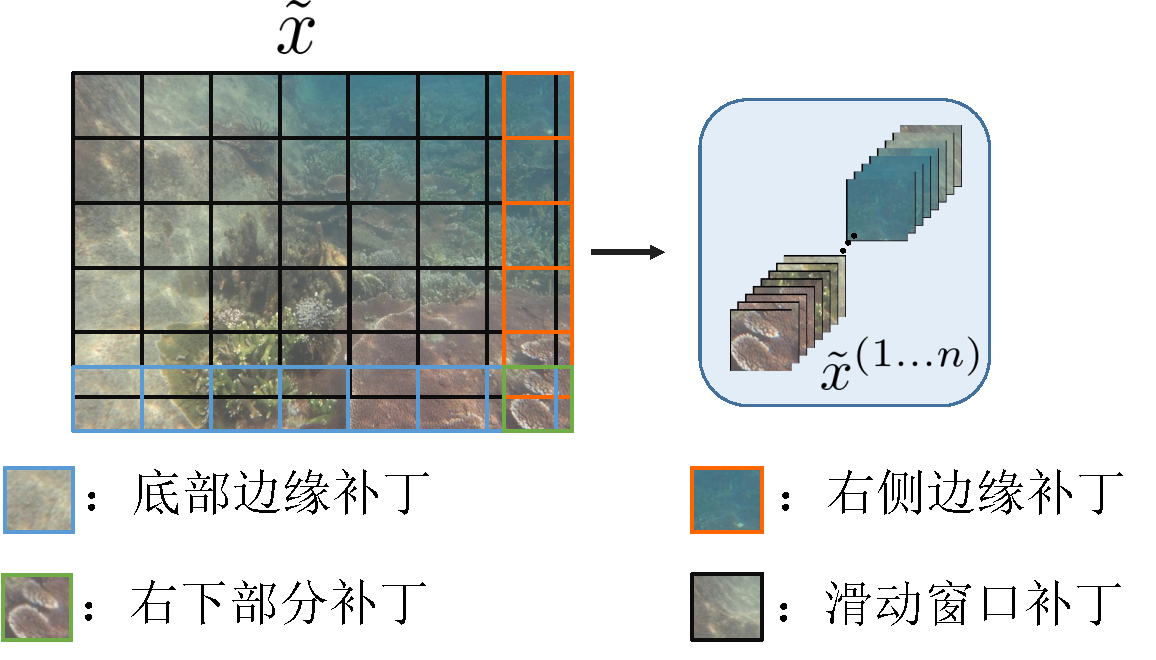
\includegraphics[width=0.8\textwidth]{figures/ch3/patch.pdf}
    \caption{水下退化图像的补丁分解示例(在滑动窗口步长$s$等于补丁大小$p$时,除边缘区域外,补丁不重叠)。}
    \label{img:patch}
\end{figure}


\subsection{基于条件去噪的采样过程}

条件扩散模型在生成任务中表现出卓越的性能,被广泛应用于图像编辑和恢复任务\cite{cDDPM} \cite{rst_DDPM}。
本章利用条件扩散模型的基本原理将退化的水下图像作为条件信息引入扩散模型采样过程中,从而确保生成结果的保真度和对目标图像特性的精确还原。
\begin{figure}
    \centering
    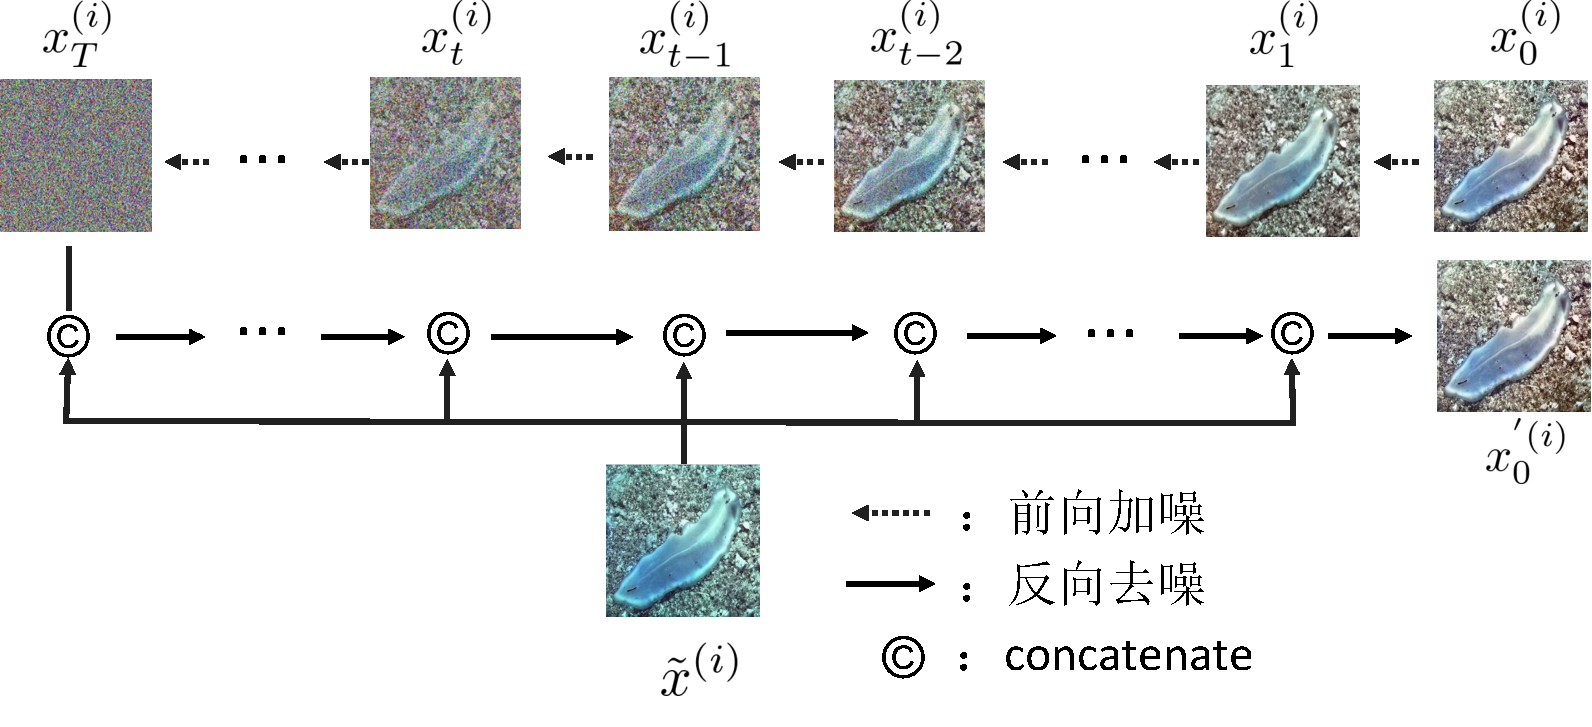
\includegraphics[width=0.8\textwidth]{figures/ch3/cond_ddpm.pdf}
    \caption{基于条件去噪的采样过程示意图。}
    \label{img:cond_ddpm}
\end{figure}

如图 \ref{img:cond_ddpm} 所示,在采样过程中,模型将退化的水下图像补丁 $\tilde{\mathbf{x}}^{(i)}$ 与当前时间步的输入噪声补丁 $\mathbf{x}^{(i)}_t$ 在通道维度上进行拼接,
生成一个六通道的组合图像。该组合图像随后被输入到噪声估计网络中,以学习条件下的噪声分布。
这一设计能够有效地结合输入噪声与退化图像信息,指导模型生成具有高保真度的去噪图像。

如算法 \ref{alg:training} 所示,训练过程中首先确定一幅完整图像的所有补丁位置掩码 $\bm{P}$,
然后随机选择一个补丁编号 $i$,以获取对应的水下清晰图像补丁 $\mathbf{x}_0^{(i)}$ 和退化的条件图像补丁 $\tilde{\mathbf{x}}^{(i)}$。
这种随机选择策略有效增加了训练数据的多样性,并降低了模型对特定补丁位置的过拟合风险。

在每次迭代中,执行以下步骤:
(1)从时间步集合 $T$ 中随机采样一个时间步长$t \sim \text{Uniform}\{1,\ldots,T\}$。
(2)从标准正态分布中生成噪声 $\bm{\epsilon}_t \sim \mathcal{N}(\mathbf{0}, \mathbf{I})$。
(3)根据公式\eqref{eq:x0_xt_patch},将噪声添加到清晰补丁 $\mathbf{x}_0^{(i)}$:
\begin{equation}
\label{eq:x0_xt_patch}
    \mathbf{x}_t^{(i)} = \sqrt{\bar{\alpha}_t} \mathbf{x}_0^{(i)} + \sqrt{1 - \bar{\alpha}_t} \bm{\epsilon}_t
\end{equation}

利用梯度下降算法训练的核心是优化模型参数 $\theta$,使其能够准确预测噪声 $\bm{\epsilon}_\theta$。目标是最小化以下损失函数:
\begin{equation}
    \nabla_{\theta}\vert\vert\bm{\epsilon}_t -  \bm{\epsilon}_{\theta}(\sqrt{\bar{\alpha}_t}\mathbf{x}_0^{(i)}+\sqrt{1-\bar{\alpha}_t}\bm{\epsilon}_t\,,\tilde{\mathbf{x}}^{(i)},t)\vert\vert^2
\end{equation}

\begin{algorithm}[ht]
    \SetAlgoLined
    \KwIn{干净图像 $\bm{X}_0$ 和退化图像 $\bm{\tilde{X}}$}
    \KwOut{训练后的模型参数 $\theta$}
  
    $n \leftarrow P.\text{length}$\;
    \Repeat{收敛}{
      随机从不同的补丁位置采样一个补丁ID $i \in \{1, 2, 3, \ldots, n\}$\;
      $\mathbf{x}_0^{(i)} \leftarrow \text{Crop}(\bm{P}_i \circ \bm{X}_0)$\;
      $\tilde{\mathbf{x}}^{(i)} \leftarrow \text{Crop}(\bm{P}_i \circ \bm{\tilde{X}})$\;
      $t \sim \text{Uniform}\{1, \ldots, T\}$ 且 $\bm{\epsilon}_t \sim \mathcal{N}(\mathbf{0}, \mathbf{I})$\;
      按以下目标执行一次梯度下降优化:\\
      \quad $\nabla_{\theta} \Vert \bm{\epsilon}_t - \bm{\epsilon}_{\theta}(\sqrt{\bar{\alpha}_t}\mathbf{x}_0^{(i)} + \sqrt{1 - \bar{\alpha}_t}\bm{\epsilon}_t, \tilde{\mathbf{x}}^{(i)}, t) \Vert^2$\;
    }
    \caption{训练}
    \label{alg:training}
  \end{algorithm}

如算法 \ref{alg:inference} 所示,采样过程中将退化的水下图像 $\tilde{\bm{X}}$ 作为条件信息,为模型提供参考。
采样图像 $\bm{X}_t$ 的初始状态为标准正态分布随机噪声:$\bm{X}_t \sim \mathcal{N}(\mathbf{0}, \mathbf{I})$。
在每个时间步 $s$ 中,通过退化图像补丁的指导,逐步去除噪声,生成最终清晰图像 $\bm{X}_t$。

% 对于基于补丁的DDIM采样器来说,其后向采样公式\eqref{eq:p}更新为:
% \begin{equation}
% \begin{split}
%     \label{eq:ddim}
%      \mathbf{x}^{(i)}_{t-1} =& \sqrt{\bar{\alpha}_{t-1}}\left(\frac{\mathbf{x}^{(i)}_t-\sqrt{1-\bar{\alpha}_t} \cdot \boldsymbol{\epsilon}_\theta\left(\mathbf{x}^{(i)}_t, t\right)}{\sqrt{\bar{\alpha}_t}}\right) \\
%      + &\sqrt{1-\bar{\alpha}_{t-1}} \cdot \epsilon_\theta\left(\mathbf{x}^{(i)}_t, t\right)
% \end{split}
% \end{equation}

对于采样过程,如果将采样步骤数设置为 $S$,每个时间步对应一个噪声去除阶段 $t$ 和 $t_{\text{next}}$,采样过程的主要步骤如下:
(1)首先从 $n$ 个补丁掩码列表 $P$ 中,提取当前图像补丁 $\mathbf{x}_t^{(i)}$ 和条件补丁 $\tilde{\mathbf{x}}^{(i)}$。
使用训练好的噪声估计网络 $\bm{\epsilon}_\theta$,为每个补丁单独预测当前时间步的噪声补丁 $\bm{\epsilon}_\theta\left(\mathbf{x}_t^{(i)}, \tilde{\mathbf{x}}^{(i)}, t\right)$;
(2)将每个补丁的噪声预测值累加到全局噪声估计矩阵 $\bm{\hat{\epsilon}}_t$,同时更新权重矩阵 $\mathbf{M}$,用于记录每个像素的累计权重;
(3)使用逐元素除法计算全局平均噪声估计:$\bm{\hat{\epsilon}}_t \leftarrow \bm{\hat{\epsilon}}_t \oslash \mathbf{M}$;
(4)最后根据估计的全局噪声 $\bm{\hat{\epsilon}}_t$,按照公式\eqref{eq:x0_xt}更新当前时间步的图像 $\bm{X}t$。
重复上述步骤直至所有时间步 $S$ 完成,最终返回清晰图像 $\bm{X}_t$,如算法\ref{alg:inference}所示。
\begin{algorithm}[ht]
    \SetAlgoLined
    \KwIn{退化图像 $\tilde{\bm{X}}$,隐式采样时间步数 $S$}
    \KwOut{采样后的图像 $\bm{X}_t$}
  
    $\bm{X}_{t} \sim \mathcal{N}(\mathbf{0}, \mathbf{I})$\;
    \For{$s = S,\ldots,1$}{
      $t \leftarrow (s-1) \cdot T / S + 1$\;
      \eIf{$s > 1$}{
        $t_{\text{next}} \leftarrow (s-2) \cdot T / S + 1$\;
      }{
        $t_{\text{next}} \leftarrow 0$\;
      }
      $\bm{\hat{\epsilon}}_t \leftarrow \mathbf{0}$\;
      $\mathbf{M} \leftarrow \mathbf{0}$\;
      \For{$i = 1,\ldots,n$}{
        $\mathbf{x}_t^{(i)} \leftarrow \text{Crop}(\mathbf{P}_i \circ \bm{X}_t)$\;
        $\tilde{\mathbf{x}}^{(i)} \leftarrow \text{Crop}(\mathbf{P}_i \circ \tilde{\bm{X}})$\;
        $\bm{\hat{\epsilon}}_t \leftarrow \bm{\hat{\epsilon}}_t + \mathbf{P}_i \cdot \bm{\epsilon}_{\theta}(\mathbf{x}_t^{(i)}, \tilde{\mathbf{x}}^{(i)}, t)$\;
        $\mathbf{M} \leftarrow \mathbf{M} + \mathbf{P}_i$\;
      }
      $\bm{\hat{\epsilon}}_t \leftarrow \bm{\hat{\epsilon}}_t \oslash \mathbf{M}$  \tcp* {$\oslash$: 元素级除法}
      $X_{t} \leftarrow \sqrt{\bar{\alpha}_{t_{\text{next}}}} \left(\frac{X_t - \sqrt{1 - \bar{\alpha}_t} \cdot \bm{\hat{\epsilon}}_t}{\sqrt{\bar{\alpha}_t}}\right) + \sqrt{1 - \bar{\alpha}_{t_{\text{next}}}} \cdot \bm{\hat{\epsilon}}_t$\;
    }
    \Return $\bm{X}_t$\;
    \caption{采样}
    \label{alg:inference}
  \end{algorithm}

\section{噪声估计网络结构}
目前去噪扩散模型的噪声估计网络大多基于 U-Net \cite{unet}架构,
本章分别通过修改和引入残差模块和注意力机制,设计了一种针对图像补丁的噪声估计网络。

如图 \ref{img:network} 所示,噪声估计网络采用带有跳跃连接的编码器-解码器架构,其输入为当前时间步 $t$ 的图像补丁 $\mathbf{x}^{(i)}_t$ 和对应的条件补丁 $\tilde{\mathbf{x}}^{(i)}$拼接形成的六通道数据。经过初始卷积操作后,输入被送入编码器进行特征提取,结果解码器生成预测的结果$\boldsymbol{\epsilon}_\theta(\mathbf{x}_t, t)$。
\begin{figure}[ht]
    \centering 
    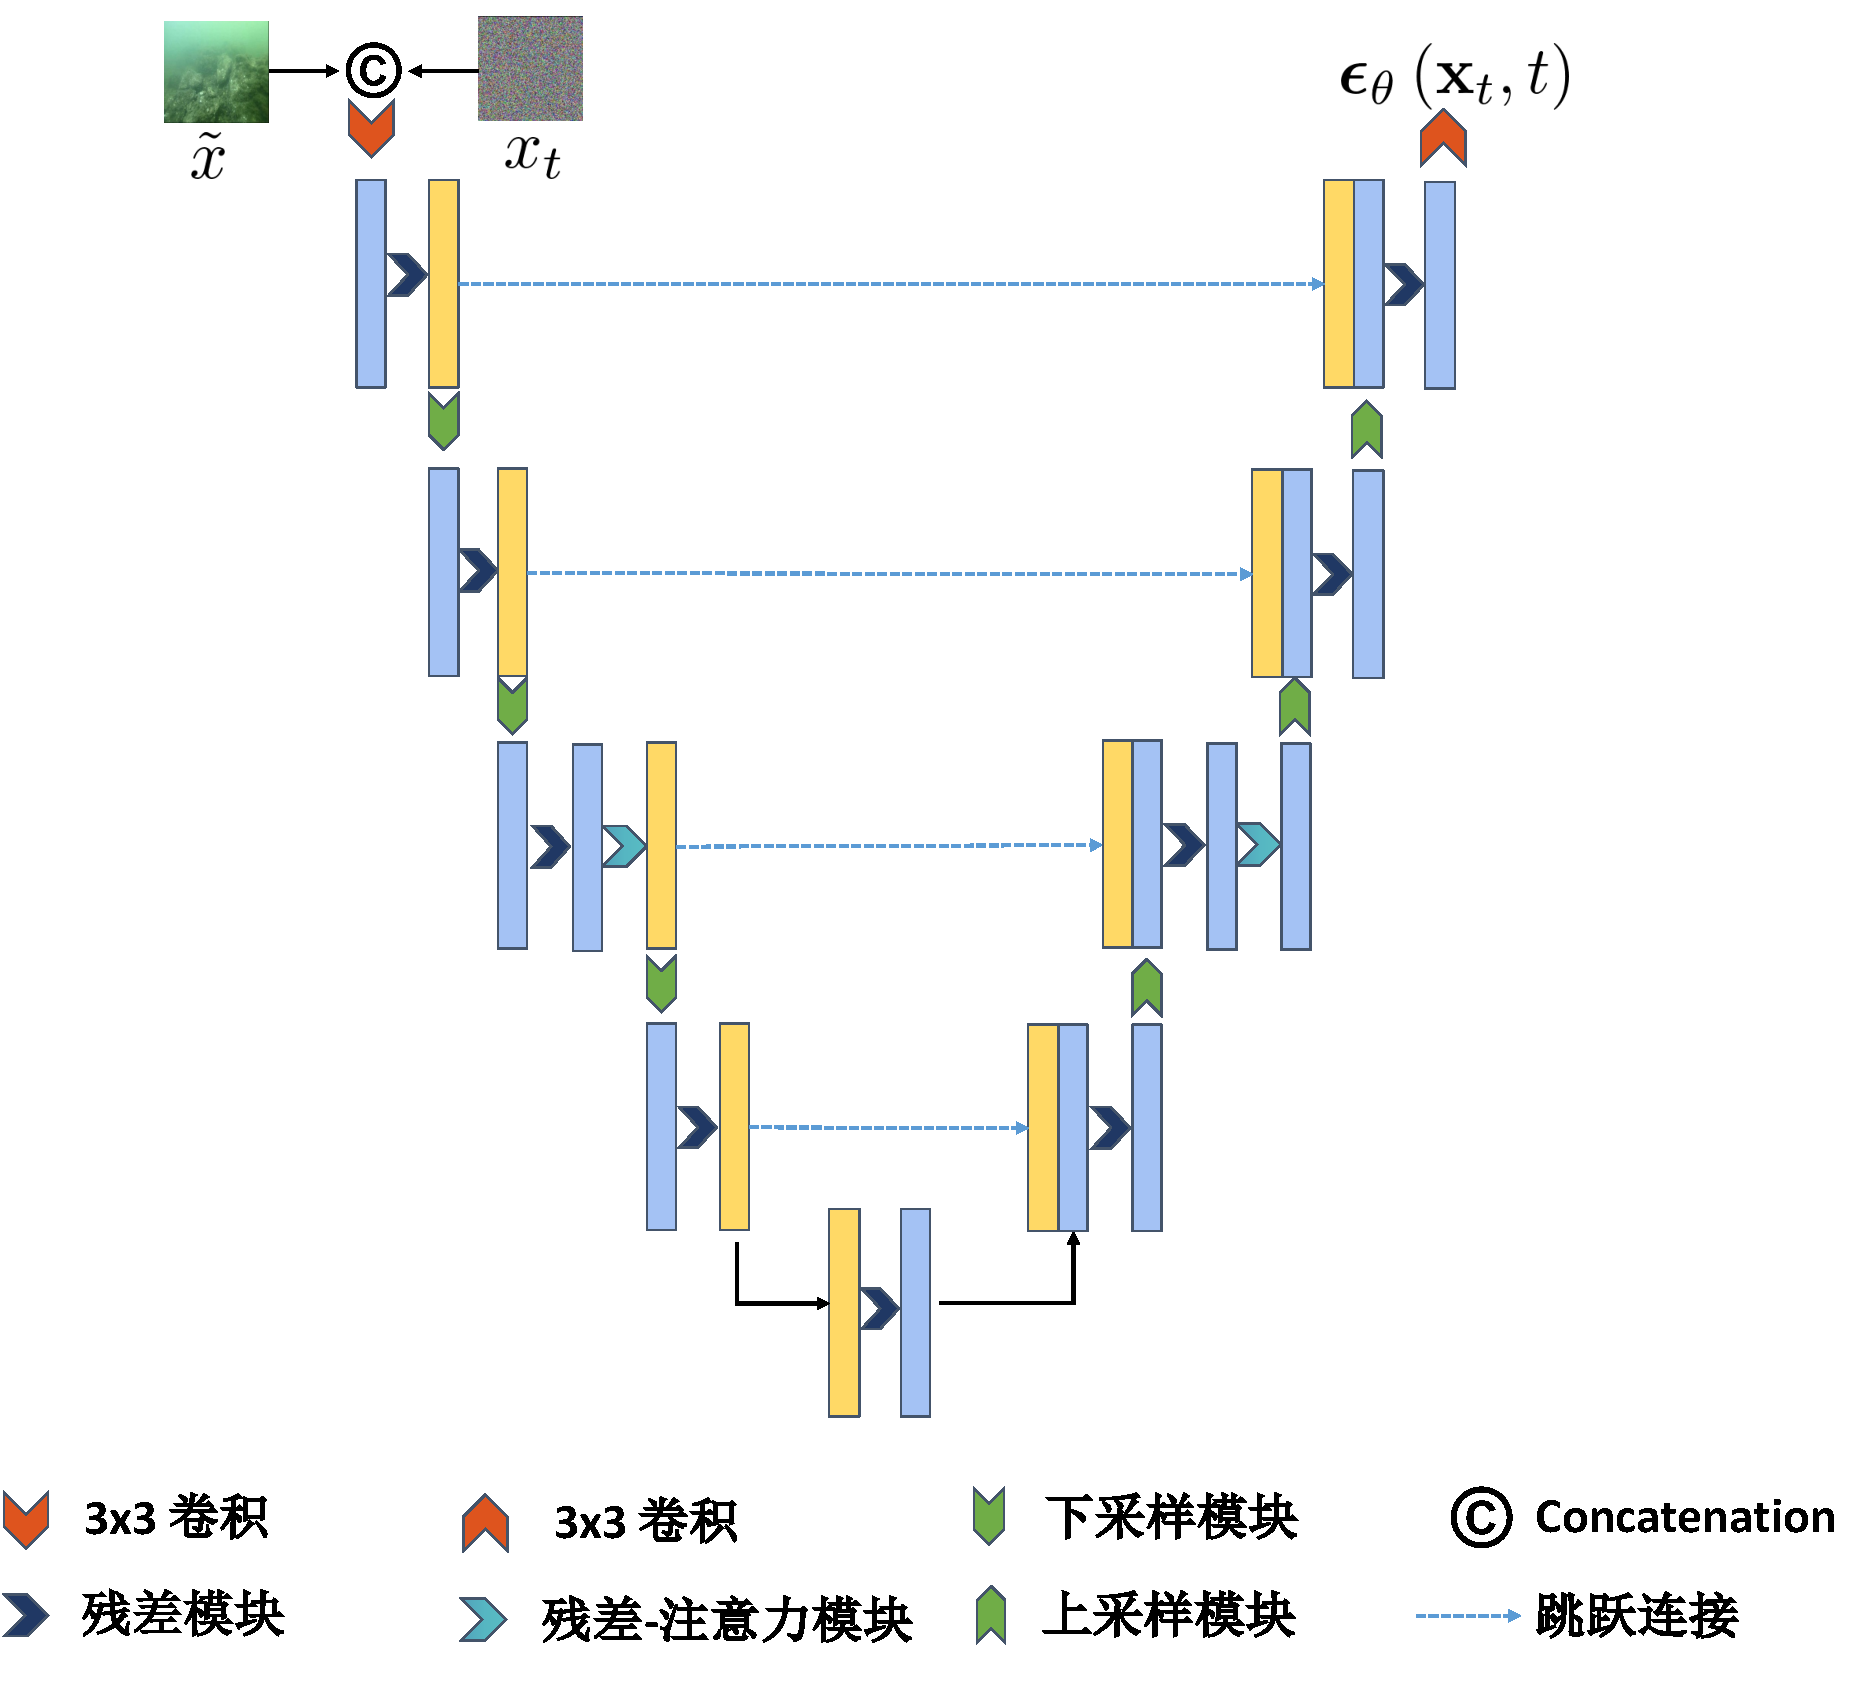
\includegraphics[width=0.8\textwidth]{figures/ch3/network.pdf}
    \caption{去噪生成网络结构示意图。}
    \label{img:network}
\end{figure}

\subsection{残差模块的特征处理}
特征处理是深度学习模型中提升特征表达能力的重要步骤,尤其是在复杂任务中,深层次的特征处理可以有效提高模型的学习能力。
残差网络(ResNet)\cite{resnet}在特征处理任务中发挥了重要作用。通过引入跨层残差连接,ResNet 缓解了深层网络中的梯度消失问题,并显著提升了特征提取的效率和精度。
本章设计的残差模块在ResNet基础上,添加了时间步的嵌入信息,如\ref{img:module}所示:
在每个残差模块中都加入一个经过正弦-余弦位置编码(sin-cos positional encoding)处理的时间步嵌入信息,
该嵌入信息经过全连接层后,与上一层的特征融合,提供时间步的相关性支持。
在卷积操作之前,模块依次执行组归一化(Group Normalization)、非线性激活函数(ReLU)和 Dropout 操作。
卷积操作后的输出会与前一层输入结合,实现跨层的残差连接。
这种设计既提升了特征的表达能力,又通过残差路径有效缓解了梯度消失问题,使模型能够更深层次地学习复杂特征。

\subsection{残差注意力模块的深度融合}
注意力机制是近年来深度学习中广泛应用的一种方法,通过捕捉特征中的全局依赖关系,显著增强了模型对关键特征的表达能力。
在本章中,我们引入了残差-注意力模块(Residual-Attention Module)以进一步提升模型的特征提取能力,
尤其是在编码器和解码器中特定分辨率为 $16 \times 16$ 的层中(如图\ref{img:network})。残差注意力模块详细设计如下:
如图\ref{img:module}所示,首先对上一层输入特征进行组归一化,确保特征分布的一致性,
再经过自注意力机制捕捉输入特征中不同位置之间的全局依赖关系,
之后将经过自注意力处理的特征输入一个 $1 \times 1$ 的卷积层,用作残差连接的Shortcut层。
最后通过残差连接,将卷积层的输出与原始输入特征融合。

类似于 Transformer 中的注意力机制 \cite{2017attention},通过引入残差路径,模块不仅增强了全局特征的感知能力,还避免了深层网络中的梯度消失问题。
残差-注意力模块的引入使模型能够在局部卷积之外关注更广范围的特征关系。特别是在处理复杂图像结构或需要全局特征分析时,该模块展现出了显著优势。
结合编码器和解码器的联合作用,模型能够更加准确地估计噪声,生成高质量的结果。

\subsection{可学习的采样策略}
编码器的核心任务是逐步压缩输入特征的空间分辨率,以提取高层次特征并为解码阶段提供丰富的语义信息。
如图 \ref{img:module} 所示,本章设计的编码器中的下采样并未采用传统的池化操作,而是用步长为 2 的卷积操作代替。这种设计使下采样过程成为一个可学习的阶段,使网络能够自主优化特征压缩方式,从而更加灵活地适应输入数据的特点。

解码器通过逐步上采样还原特征的空间分辨率,最终输出预测的噪声估计结果 $\boldsymbol{\epsilon}_\theta(\mathbf{x}_t, t)$。
上采样操作的实现方式主要包括两种:(1)线性插值结合卷积:通过插值扩展特征图尺寸,然后使用卷积操作进一步优化特征。(2)反卷积:直接通过反卷积操作增加特征的空间分辨率。
如图 \ref{img:module} 所示,本章选择了反卷积方式进行上采样,
通过反卷积操作从瓶颈层的低分辨率特征图逐步还原到输入图像的原始尺寸。
相比插值结合卷积的方式,反卷积具有更强的学习能力,能够动态调整特征映射的还原方式。

此外,类似-Net的设计,解码器中通过四次跳跃连接(Skip Connections),将编码器中对应分辨率的特征直接传递到解码器,弥补了下采样过程中可能丢失的信息。
这种设计显著提高了生成结果的质量和一致性。算法整体采样过程如图\ref{img:sample_process}所示。
\begin{figure}[ht]
    \centering
    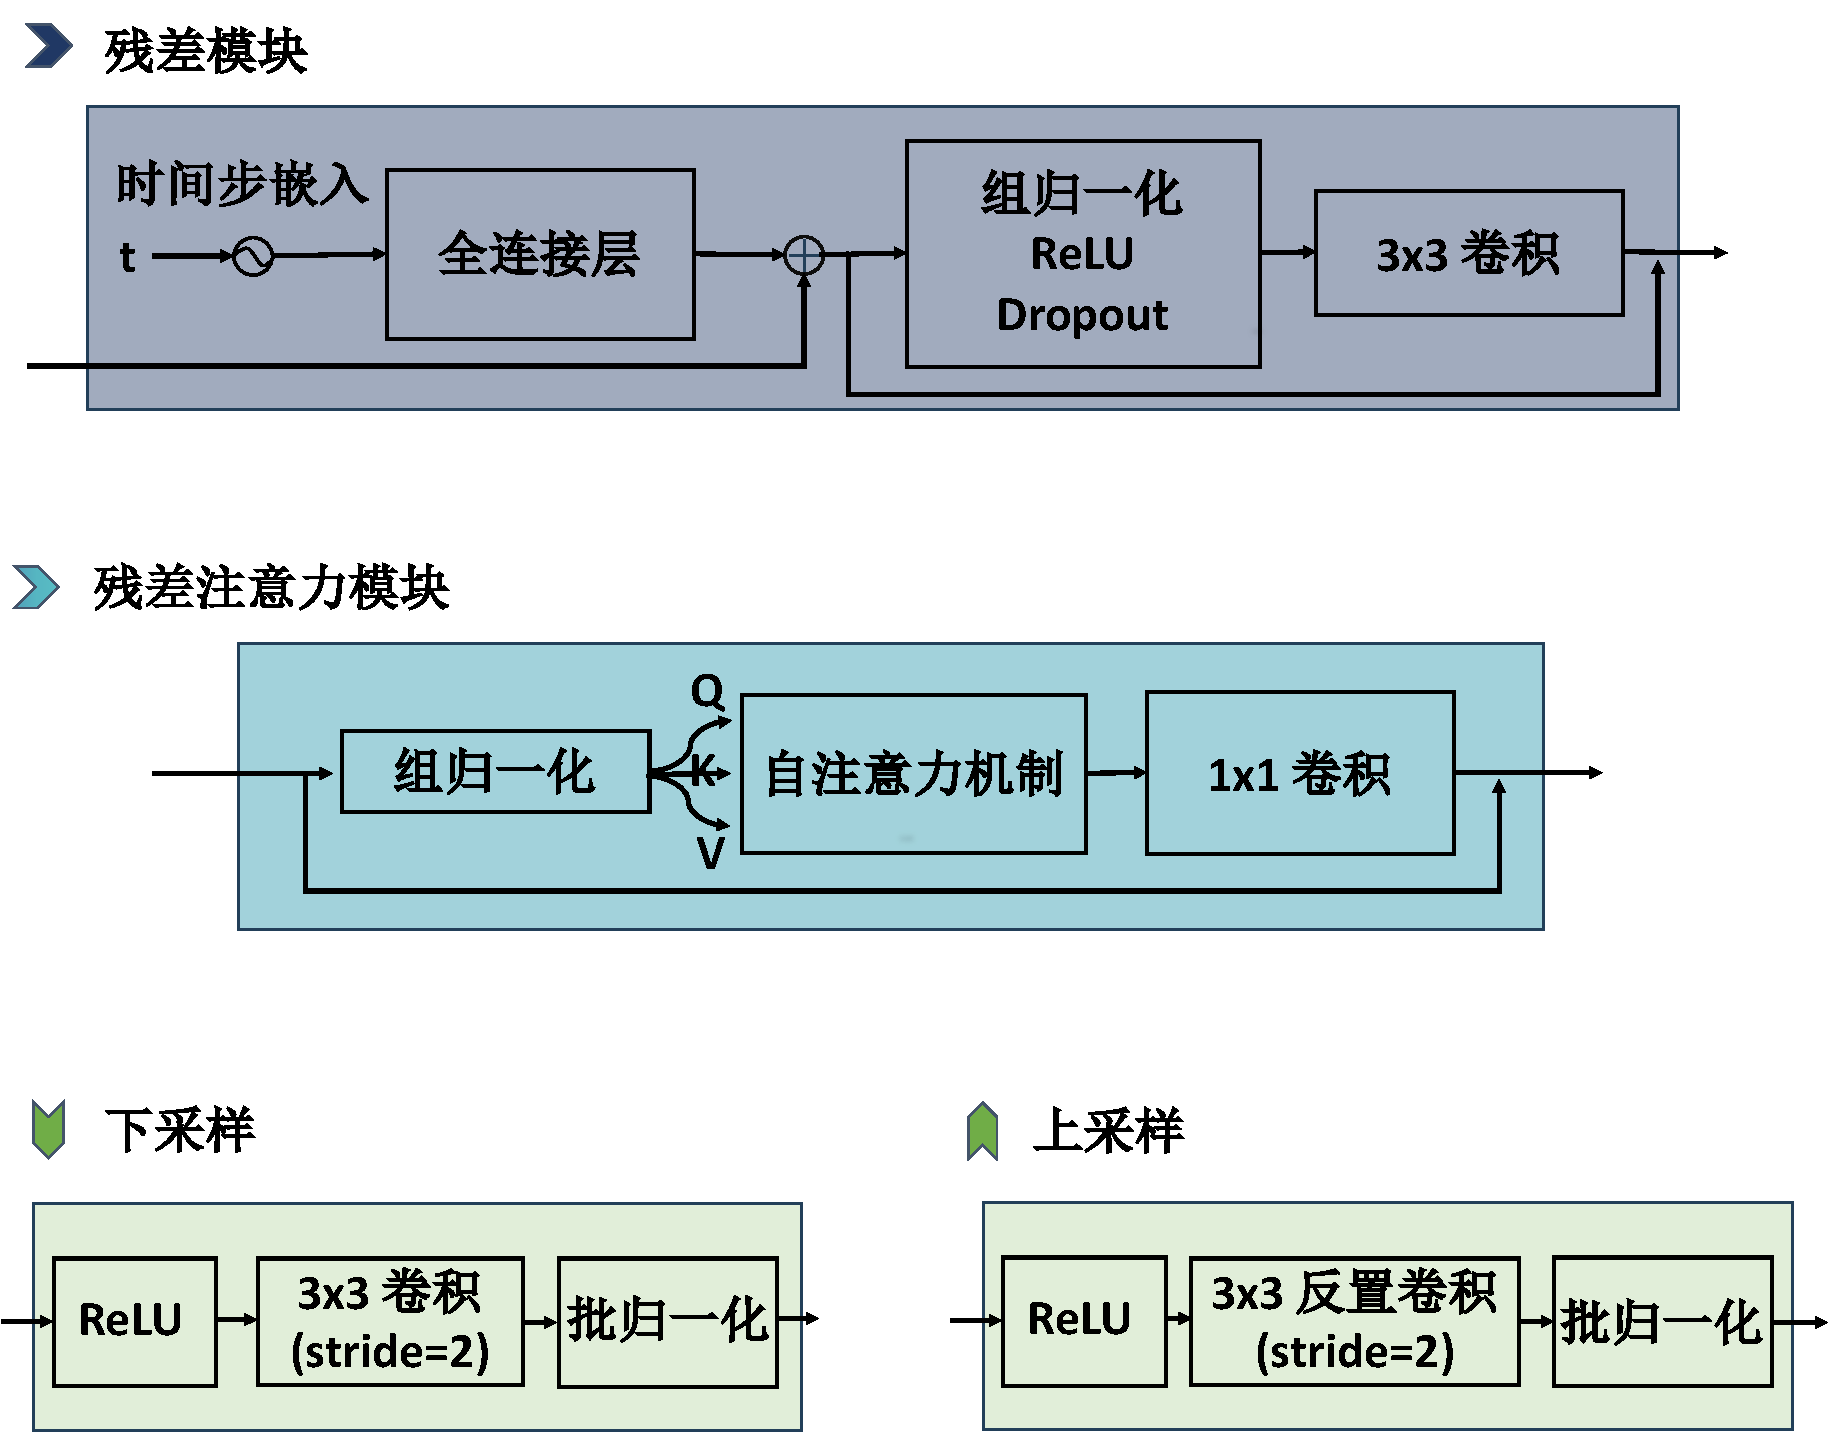
\includegraphics[width=0.8\textwidth]{figures/ch3/module.pdf}
    \caption{各模块示意图。}
    \label{img:module}
    \vspace{0.4cm}
\end{figure}

\begin{figure}[ht]
    \centering
    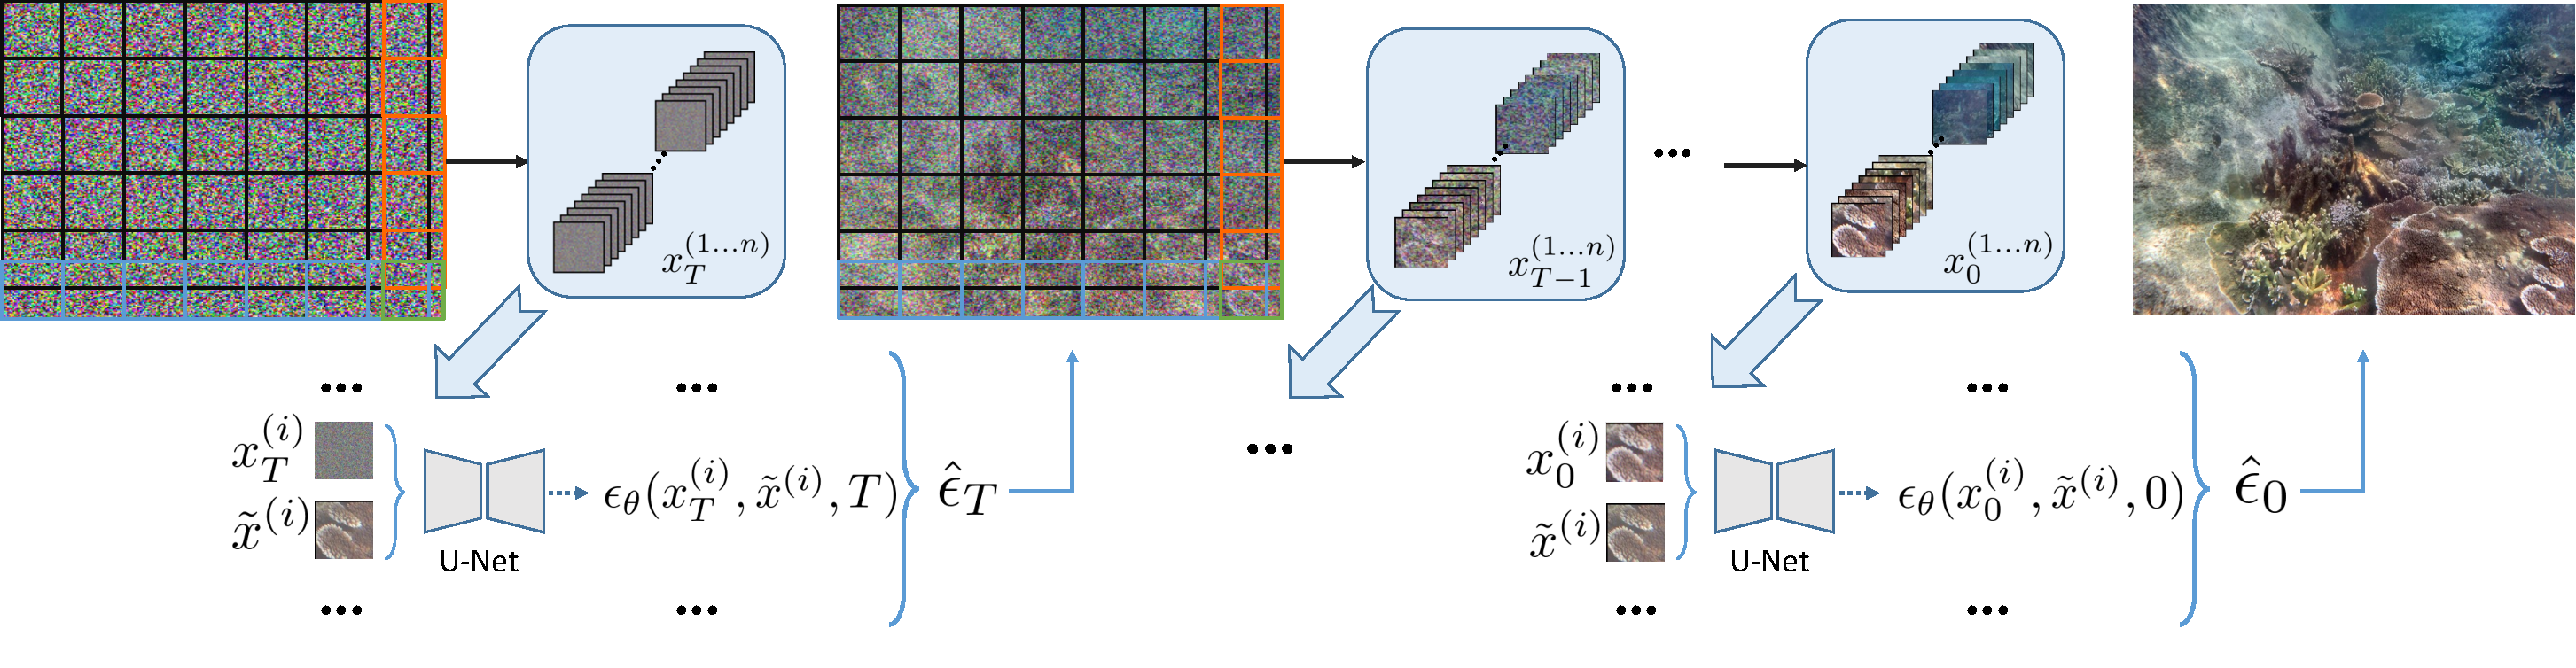
\includegraphics[width=0.98\textwidth]{figures/ch3/sample_process.pdf}
    \caption{各模块示意图。}
    \label{img:sample_process}
\end{figure} 


\section{实验结果与分析}
\subsection{实验设置}
实验选用了两个开源的水下图像增强数据集——EUVP \cite{funie_gan} 和 UIEB \cite{uieb} 作为基准数据集,
其中EUVP 数据集包含 11,435 对配对的水下图像,涵盖三种不同的风格,图像分辨率主要为 $256 \times 256$,
UIEB 数据集包含 890 对配对图像以及 60 张无参考图像。
该数据集的分辨率相比EUVP较高,图 \ref{img:scatter} 展示了两个数据集分辨率的分布情况。
训练集和测试集的划分见表 \ref{tab:dataset-split}。
\begin{figure}[ht]
    \centering
    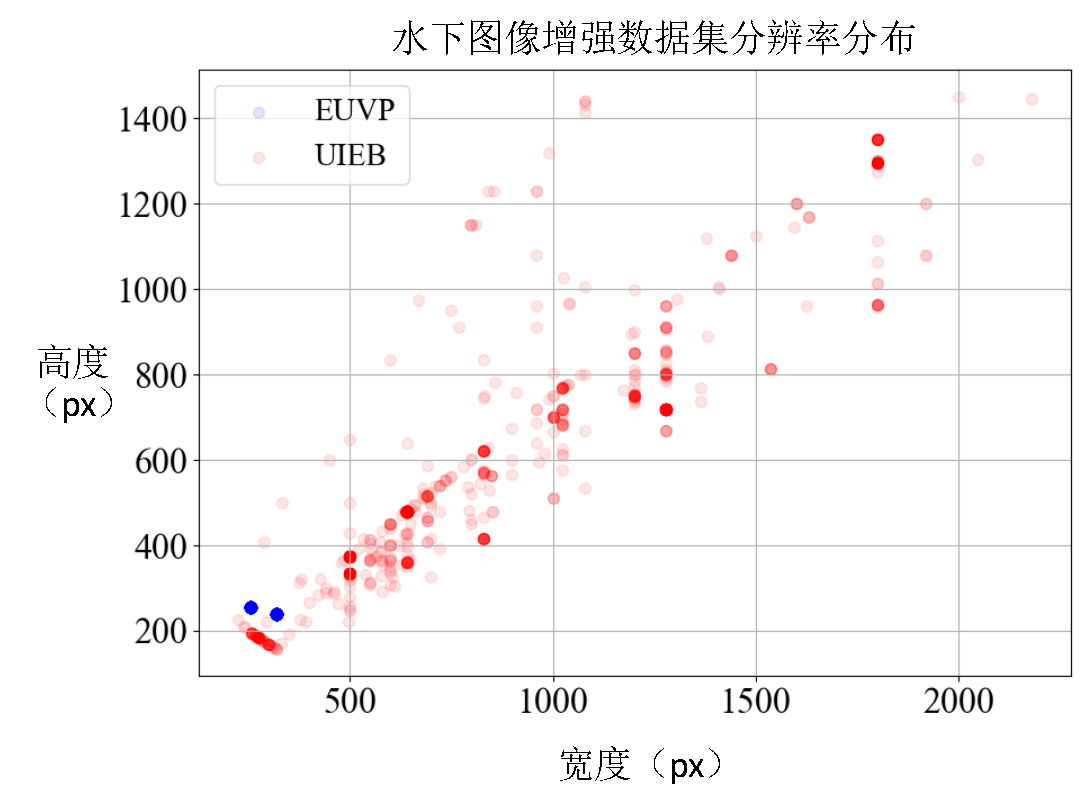
\includegraphics[width=0.8\textwidth]{figures/ch3/scatter.pdf}
    \caption{EUVP 和 UIEB 数据集中图像的分辨率分布。}
    \label{img:scatter}
\end{figure}

\begin{table}[ht]
	\vspace{-0.4mm}
	\centering
	\caption{\label{tab:dataset-split}数据集划分(成对图像)。}
	\vspace{-2mm}
	\setlength{\tabcolsep}{2.6mm}{
		\begin{tabular}{lccc}
			\toprule
			\specialrule{0em}{1pt}{1pt}
			\textbf{数据集}  & \textbf{训练集}  & \textbf{测试集} & \textbf{共计} \\
			\hline
			\specialrule{0em}{1pt}{1pt}
			EUVP (paired) \cite{funie_gan}  & $8,363$  & $3,072$  & $11,435$\\
			\specialrule{0em}{1pt}{1pt}
                UIEB (paired) \cite{uieb}  & $678$  & $212$  & $890$\\
			\bottomrule
	\end{tabular}}
	\vspace{-1mm}
\end{table}   

实验基于 PyTorch 框架,在 NVIDIA RTX3060 GPU 上进行。
整个训练过程迭代 500,000 次,批量大小为 8。图像补丁大小设置为 $64 \times 64$,与噪声估计网络的输入维度一致。
优化器采用 Adam \cite{kingma2017adam},学习率为 $2 \times 10^{-4}$。

去噪扩散模型采样过程的总采样步数 $T$ 设置为 1000,基于去噪扩散隐式模型的采样推理步数 $S$ 设置为 20,以加速推理。
方差调度参数 $\beta_i$ 采用线性变化,从 0.0001 逐步增加到 0.02。

\subsection{定量评价} \label{sec:quantitative}
在图像恢复领域,对恢复结果进行定量评价至关重要。本章选取了两种在图像恢复领域被广泛使用的峰值信噪比和结构相似性指数来对不同算法生成结果进行定量比较。
同时,由于水下图像的特殊性,本章还选取了专门的水下图像质量指标来对结果进行无参考质量评价。

(1)峰值信噪比(Peak Signal to Noise Ratio,PSNR):PSNR是一种客观评价图像质量的重要指标,它通过比较图像信号的最大值与背景噪声的强弱来评估图像质量。
该指标对光照误差敏感,能有效反映图像质量,峰值信噪比越高,图像质量通常越好。
PSNR 首先统计了参考图像和增强图像之间的均方误差$\mathrm{MSE}$:
\begin{equation}
    \mathrm{MSE} = \frac{1}{N} \sum_{i=1}^{N} (I(i) - K(i))^2
\end{equation}

其中,$I$ 和 $K$ 分别表示参考图像和增强图像,$N$ 表示图像的像素总数。PSNR对均方误差的结果进了一定的标准化,计算方式为:
\begin{equation}
    \mathrm{PSNR} =10 \times \log _{10} \frac{(\mathrm{MAXI})^2}{\mathrm{MSE}}
\end{equation}

其中,$\mathrm{MAXI}$ 为图像的最大像素值,表示像素值的动态范围,对于8位图像,$\mathrm{MAXI}=255$。

(2)结构相似性指数(SSIM) \cite{ssim}:SSIM通过比较图像之间的多个视觉要素来计算损失,包括亮度$l$、对比度$c$和结构$s$三个方面评价图像质量。
其中,亮度测量需要计算参考图像的像素平均值$\mu_x$和增强图像的像素平均值$\mu_y$:
\begin{equation}
    \mu_x = \frac{1}{N} \sum_{i=1}^{N} I(i) , \quad \mu_y = \frac{1}{N} \sum_{i=1}^{N} K(i)
\end{equation}

其中,$I$ 表示参考图像,$K$ 表示增强图像,$N$ 表示图像的像素总数。
亮度评价指标的计算公式为:
\begin{equation}
    l(x, y) = \frac{2\mu_x\mu_y + c_1}{\mu_x^2 + \mu_y^2 + c_1}
\end{equation}

对比度评价指标的计算公式为:
\begin{equation}
    c(x, y) = \frac{2\sigma_x\sigma_y + c_2}{\sigma_x^2 + \sigma_y^2 + c_2}
\end{equation}

结构评价指标的计算公式为:
\begin{equation}
    s(x, y) = \frac{{\sigma_{xy} + c_3}}{{\sigma_x\sigma_y + c_3}}
\end{equation}

其中,常数$c_1=(255\times0.01)^2$、$c_2=(255\times0.03)^2$、$c_3=(255\times0.015)^2$ 是稳定因子,
$\sigma_x$ 和 $\sigma_y$ 分别表示参考图像和增强图像的标准差,$\sigma_{xy}$ 表示协方差:
\begin{equation}
    \begin{split}
    \sigma_{xy} &= \frac{1}{N} \sum_{i=1}^{N} (I(i) - \mu_x)(K(i) - \mu_y), \\
    \sigma_x^2 &= \frac{1}{N} \sum_{i=1}^{N} (I(i) - \mu_x)^2, \\
    \sigma_y^2 &= \frac{1}{N} \sum_{i=1}^{N} (K(i) - \mu_y)^2
    \end{split}
\end{equation}

SSIM 为上面三个指标的加权平均值:
\begin{equation}
    \mathrm{SSIM} = [{{l(x,y)}^\alpha} \cdot {{c(x,y)}^\beta} \cdot {{s(x,y)}^\gamma} ]
\end{equation}

令$c_3=\frac{c_2}{2}$,$\alpha=\beta=\gamma=1$,则SSIM可以简化为:
\begin{equation}
    \mathrm{SSIM} = \frac{{(2\mu_x\mu_y + c_1)(2\sigma_{xy} + c_2)}}{{(\mu_x^2 + \mu_y^2 + c_1)(\sigma_x^2 + \sigma_y^2 + c_2)}}
\end{equation}

其中,$\mathrm{SSIM}$ 的取值范围为 $[-1, 1]$,值越大,表示图像质量与参考图像越相似,图像质量越好。

(3)水下图像质量指标(UIQM) \cite{uiqm}:UIQM是一种无参考水下图像质量评价指标,
对于水下图像来说,不同波长的衰减系数不同,导致图像存在色偏,正向散射效应往往会造成成像模糊,而后向散射效应限制了图像的对比度。
因此,UIQM综合考量了水下图像的色彩测量指标$\mathrm{UICM}$、清晰度测量指标$\mathrm{UISM}$和对比度测量指标$\mathrm{UIConM}$最为最终的评价指标。

$\mathrm{UICM}$通过分析图像的颜色通道差异来量化图像的色彩特性:
\begin{equation}
    \mathrm{UICM}=-0.0268 \times \sqrt{\mu_{RG}^2 + \mu_{YB}^2} + 0.1586 \times \sqrt{\sigma_{RG}^2 + \sigma_{YB}^2}
\end{equation}

其中,$\mu_{RG}$ 和 $\mu_{YB}$ 分别表示图像的红绿两个通道的差异均值和黄(红绿通道像素均值)蓝两个通道的差异均值,$\sigma_{RG}$ 和 $\sigma_{YB}$ 分别表示对应的方差。

$\mathrm{UISM}$ 通过分析图像的局部对比度来量化图像的清晰度,首先需要计算图像的局部对比度$\mathrm{EME}$:
\begin{equation}
    \mathrm{EME} = \frac{2}{k_1 k_2} \sum_{l=1}^{k_1} \sum_{k=1}^{k_2} \log \left( \frac{I_{\text{max},k,l}}{I_{\text{min},k,l}} \right)
\end{equation}

其中,$k_1$ 和 $k_2$ 分别表示图像的行和列的像素数,$I_{\text{max},k,l}$ 和 $I_{\text{min},k,l}$ 分别表示图像在第$k$行和第$l$列的像素最大值和最小值。
$\mathrm{UISM}$ 为$\mathrm{EME}$的在不同通道上的加权和:
\begin{equation}
    \mathrm{UISM} = 0.299 \times \mathrm{EME}_{R} + 0.587 \times \mathrm{EME}_{G} + 0.114 \times \mathrm{EME}_{B}
\end{equation}

$\mathrm{UIConM}$ 通过衡量图像中最亮和最暗部分的区分度来量化图像的对比度,其首先在图像对应灰度图像中计算平均灰度值$\mu$:
\begin{equation}
   \mu = \frac{1}{N} \sum_{i=1}^{N} x_i
\end{equation}

其中,$N$ 表示图像的像素总数,$x_i$ 表示图像的第$i$个像素的灰度值。然后计算灰度图的标准差 \(\sigma\)即为UIConM值:
\begin{equation}
    \mathrm{UIConM}=\sigma = \sqrt{\frac{1}{N} \sum_{i=1}^{N} (x_i - \mu)^2} 
\end{equation}

UIQM 是以上三种测量指标的加权和:
\begin{equation}
    \mathrm{UIQM}=c_1 \times \mathrm{UICM}+c_2 \times \mathrm{UISM}+c_3 \times \mathrm{UIConM}
\end{equation}
其中常数$c_1=0.0282$、$c_2=0.2953$、$c_3=3.5753$为权重系数。

表\ref{tab:psnr-ssim}  和表\ref{tab:uiqm} 分别展示了本章提出的水下图像增强的方法与其他方法在 PSNR、SSIM 和 UIQM 等指标上的比较结果。
其中 Ucolor\cite{ucolor}模型需要额外的传输图作为输入,
由于DCP系列方法可以生成额外的传输图,并且本章的实验包括UDCP\cite{udcp}算法,所以使用UDCP生成的传输图来评估Ucolor模型,
而Ucolor所提出的原始方法使用一般暗通道\cite{GDCP}提取所需的传输图。
实验结果表明本章提出的水下图像增强方法在多个指标上表现优越,
在有参考质量指标(PSNR 和 SSIM)方面展现了具有接近高质量参考图像水平,
在无参考指标(UIQM)上,基于去噪扩散模型的水下图像增强方法的综合表现仍处于领先地位,在提升增强图像的细节质量与全局一致性方面具有明显优势。

\begin{table*}[t]
	\footnotesize
        \captionsetup{justification=centering}
	\caption{不同方法在数据集 EUVP 和 UIEB 上的 PSNR 和 SSIM 定量结果。以红色字体显示的分数代表该行中排名最高的方法。}
	\label{tab:psnr-ssim}
	\vspace{-0.4mm}
	\centering
	\setlength{\tabcolsep}{1.01mm}{
		\renewcommand{\arraystretch}{1.1}
            \begin{tabular}{cccccccccc}
			\toprule
			数据集 & 指标 & UDCP\cite{udcp} & UGAN\cite{ugan} & FGAN\cite{funie_gan} & UWCNN\cite{uwcnn} & Ucolor\cite{ucolor} & STSC\cite{stsc} & U-shape\cite{u-shape} & Ours\\
			\hline
			\multirow{2}{*}{EUVP} & \textbf{PSNR} & $16.71$ & $27.46$ & $26.59$ & $21.56$ & $26.27$ & $20.71$ & $26.23$ & $\textcolor{red}{\textbf{30.29}}$ \\ & \textbf{SSIM} & $0.76$ & $0.87$ & $0.84$ & $0.84$ & $0.89$ & $0.83$ & $0.88$ & $\textcolor{red}{\textbf{0.92}}$ \\
            \vspace{-2mm} 
             \hspace*{\fill} \\
			% \hline
            
			\multirow{2}{*}{UIEB} & \textbf{PSNR} & $13.20$ & $21.01$ & $20.76$ & $14.86$ & $\textcolor{red}{\textbf{23.90}}$ & $21.46$ & $20.94$ & $21.34$ \\ & \textbf{SSIM}  & $0.70$ & $0.69$ & $0.68$ & $0.69$ & $0.91$ & $0.72$ & $0.62$ & $\textcolor{red}{\textbf{0.92}}$  \\
			\bottomrule
	\end{tabular}}
	\vspace{-0.4mm}
\end{table*}   % paired

\begin{table*}[t]
	%	\vspace{-4mm}
	\footnotesize
	\caption{不同方法在数据集 EUVP 和 UIEB 上的 UIQM 定量结果。以红色字体显示的分数代表该行中排名最高的方法。}
	\label{tab:uiqm}
	\vspace{-0.4mm}
	\centering
	\setlength{\tabcolsep}{1.01mm}{
		\renewcommand{\arraystretch}{1.1}
		% \begin{tabular}{c|c|ccccccc|c}
            \begin{tabular}{cccccccccc}
			\toprule
			数据集 & 指标 & UDCP\cite{udcp} & UGAN\cite{ugan} & FGAN\cite{funie_gan} & UWCNN\cite{uwcnn} & Ucolor\cite{ucolor} & STSC\cite{stsc} & U-shape\cite{u-shape} & Ours\\
			\hline
			\multirow{4}{*}{EUVP} & UICM & $\textcolor{red}{\textbf{5.85}}$ & $3.76$ & $4.54$ & $2.97$ & $3.94$ &  $5.31$ & $4.16$ & $4.67$ \\
			& UISM & $6.28$ & $7.40$ & $7.15$ & $6.85$ & $7.33$ & $\textcolor{red}{\textbf{7.41}}$ & $7.29$ & $7.25$\\
                & UIConM & $0.03$ & $0.22$ & $0.20$ & $0.29$ & $0.27$ &
            $0.28$ & $0.27$ & $\textcolor{red}{\textbf{0.30}}$\\
                 % \cline{2-10}
                & \textbf{UIQM} & $2.13$ & $3.08$ & $2.97$ & $3.15$ & $3.25$ &
            $3.34$ & $3.22$ & $\textcolor{red}{\textbf{3.35}}$ \\
            \vspace{-2mm} 
             \hspace*{\fill} \\
			% \hline
			\multirow{4}{*}{UIEB} & UICM & $\textcolor{red}{\textbf{6.70}}$ & $5.63$ & $5.44$ & $2.69$ & $5.06$ & $5.80$ & $4.91$ & $5.28$ \\
			& UISM & $5.42$ & $5.35$ & $5.24$ & $4.98$ & $6.74$ & $5.25$ & $5.32$ & $\textcolor{red}{\textbf{7.08}}$\\
                & UIConM & $0.04$ & $0.29$ & $0.29$ & $0.31$ & $0.30$ &
            $\textcolor{red}{\textbf{0.33}}$ & $0.32$ & $0.30$\\
                % \cline{2-10}
                & \textbf{UIQM} & $1.97$ & $2.77$ & $2.74$ & $2.65$ & $3.20$ &
            $2.89$ & $2.86$ & $\textcolor{red}{\textbf{3.32}}$\\
			\bottomrule
	\end{tabular}}
	\vspace{-0.4mm}
\end{table*}   

\subsection{主观评价}
如图\ref{img:scatter} 展示的 EUVP 和 UIEB 数据集中图像的分辨率分布,基准数据集中的图像分辨率大小并不一致,
而大多数基于深度学习的水下图像增强方法(如 FGAN\cite{funie_gan}、UGAN\cite{ugan}、U-shape\cite{u-shape} 和 STSC\cite{stsc})
均在固定的输入和输出尺寸下进行训练和推理。而本章方法具备更高的分辨率适应性。

如图\ref{img:visual-euvp}和图\ref{img:visual-uieb}所示,首先在$256 \times 256$ 图像分辨率尺寸下实验对比了不同方法在 EUVP 和 UIEB 数据集上的主观增强效果。
实验结果表明,本章提出的水下图像增强方法在保持图像真实感的同时,显著提升了水下物体的色彩表现。
尤其在蓝色和绿色主导的水域场景中,可以增强画面色彩饱和度和自然感。
\begin{figure}[t]
	\begin{center}
		\begin{tabular}{ccccccccc}
			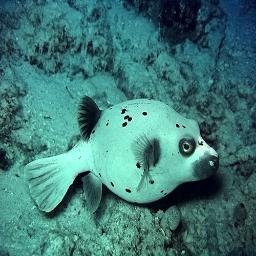
\includegraphics[width = 0.10\linewidth,height=0.10\linewidth]{figures/ch3/compare/EUVP/Input/264318_n02655020_17544.JPEG} & \hspace{-0.40cm}
			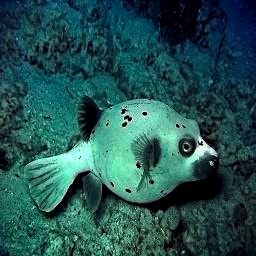
\includegraphics[width = 0.10\linewidth,height=0.10\linewidth]{figures/ch3/compare/EUVP/UDCP/264318_n02655020_17544.JPEG}  & \hspace{-0.40cm}
			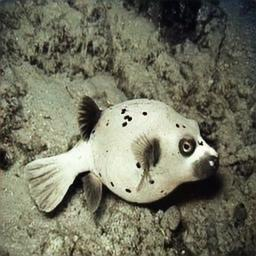
\includegraphics[width = 0.10\linewidth,height=0.10\linewidth]{figures/ch3/compare/EUVP/UGAN/264318_n02655020_17544.JPEG}  & \hspace{-0.40cm}
			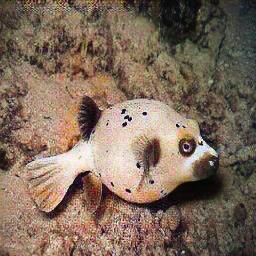
\includegraphics[width = 0.10\linewidth,height=0.10\linewidth]{figures/ch3/compare/EUVP/FGAN/264318_n02655020_17544.JPEG}  & \hspace{-0.40cm}
			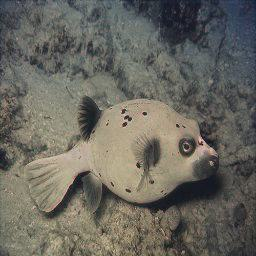
\includegraphics[width = 0.10\linewidth,height=0.10\linewidth]{figures/ch3/compare/EUVP/UWCNN/264318_n02655020_17544.JPEG} & \hspace{-0.40cm}
			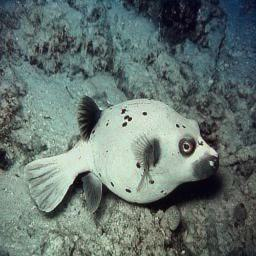
\includegraphics[width = 0.10\linewidth,height=0.10\linewidth]{figures/ch3/compare/EUVP/Ucolor/264318_n02655020_17544.JPEG}& \hspace{-0.40cm}
			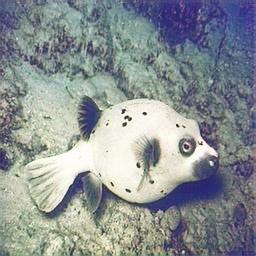
\includegraphics[width = 0.10\linewidth,height=0.10\linewidth]{figures/ch3/compare/EUVP/STSC/264318_n02655020_17544.JPEG}  & \hspace{-0.40cm}
			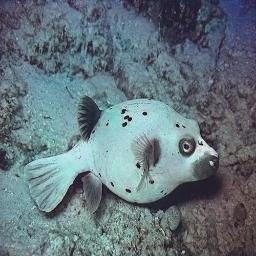
\includegraphics[width = 0.10\linewidth,height=0.10\linewidth]{figures/ch3/compare/EUVP/Ushape/264318_n02655020_17544.JPEG}& \hspace{-0.40cm} 
            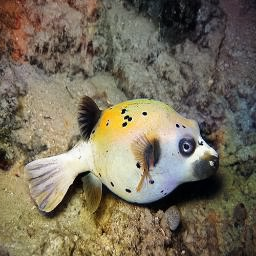
\includegraphics[width = 0.10\linewidth,height=0.10\linewidth]{figures/ch3/compare/EUVP/Ours/264318_n02655020_17544..png}  \\
                
            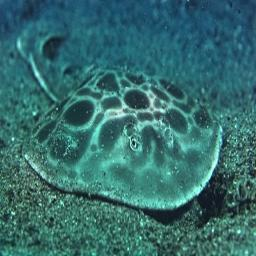
\includegraphics[width = 0.10\linewidth,height=0.10\linewidth]{figures/ch3/compare/EUVP/Input/265613_n01496331_8134.JPEG}  & \hspace{-0.40cm}
			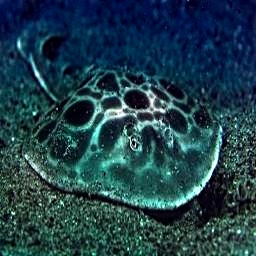
\includegraphics[width = 0.10\linewidth,height=0.10\linewidth]{figures/ch3/compare/EUVP/UDCP/265613_n01496331_8134.JPEG}   & \hspace{-0.40cm}
			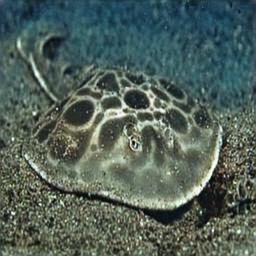
\includegraphics[width = 0.10\linewidth,height=0.10\linewidth]{figures/ch3/compare/EUVP/UGAN/265613_n01496331_8134.JPEG}   & \hspace{-0.40cm}
			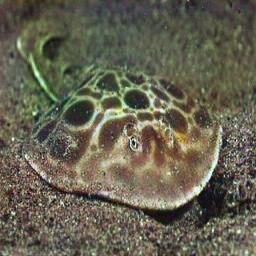
\includegraphics[width = 0.10\linewidth,height=0.10\linewidth]{figures/ch3/compare/EUVP/FGAN/265613_n01496331_8134.JPEG}   & \hspace{-0.40cm}
			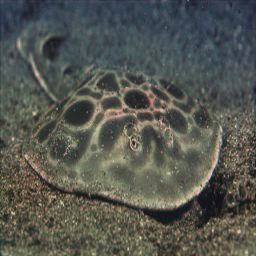
\includegraphics[width = 0.10\linewidth,height=0.10\linewidth]{figures/ch3/compare/EUVP/UWCNN/265613_n01496331_8134.JPEG}  & \hspace{-0.40cm}
			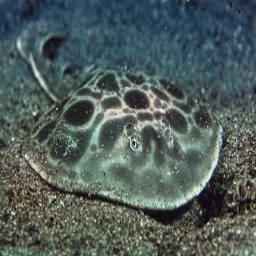
\includegraphics[width = 0.10\linewidth,height=0.10\linewidth]{figures/ch3/compare/EUVP/Ucolor/265613_n01496331_8134.JPEG} & \hspace{-0.40cm}
			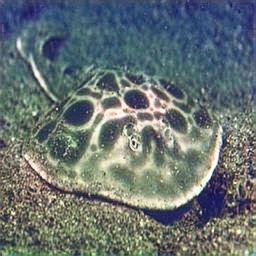
\includegraphics[width = 0.10\linewidth,height=0.10\linewidth]{figures/ch3/compare/EUVP/STSC/265613_n01496331_8134.JPEG}   & \hspace{-0.40cm}
			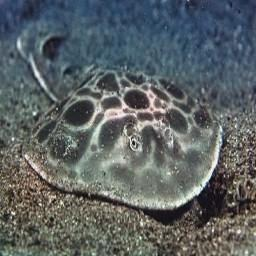
\includegraphics[width = 0.10\linewidth,height=0.10\linewidth]{figures/ch3/compare/EUVP/Ushape/265613_n01496331_8134.JPEG} & \hspace{-0.40cm}         
			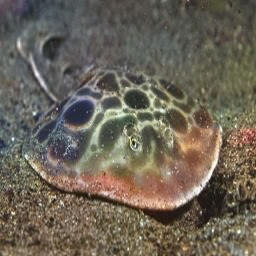
\includegraphics[width = 0.10\linewidth,height=0.10\linewidth]{figures/ch3/compare/EUVP/Ours/265613_n01496331_8134..png}   \\

            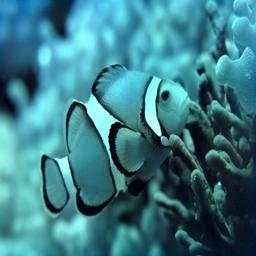
\includegraphics[width = 0.10\linewidth,height=0.10\linewidth]{figures/ch3/compare/EUVP/Input/264298_00035269.jpg}  & \hspace{-0.40cm}
			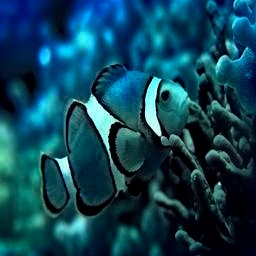
\includegraphics[width = 0.10\linewidth,height=0.10\linewidth]{figures/ch3/compare/EUVP/UDCP/264298_00035269.jpg}   & \hspace{-0.40cm}
			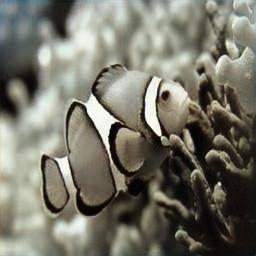
\includegraphics[width = 0.10\linewidth,height=0.10\linewidth]{figures/ch3/compare/EUVP/UGAN/264298_00035269.jpg}   & \hspace{-0.40cm}
			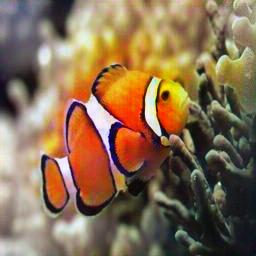
\includegraphics[width = 0.10\linewidth,height=0.10\linewidth]{figures/ch3/compare/EUVP/FGAN/264298_00035269.jpg}   & \hspace{-0.40cm}
			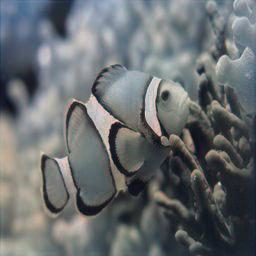
\includegraphics[width = 0.10\linewidth,height=0.10\linewidth]{figures/ch3/compare/EUVP/UWCNN/264298_00035269.jpg}  & \hspace{-0.40cm}
			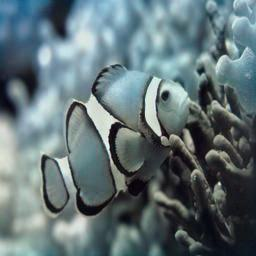
\includegraphics[width = 0.10\linewidth,height=0.10\linewidth]{figures/ch3/compare/EUVP/Ucolor/264298_00035269.jpg} & \hspace{-0.40cm}
			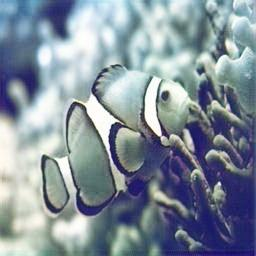
\includegraphics[width = 0.10\linewidth,height=0.10\linewidth]{figures/ch3/compare/EUVP/STSC/264298_00035269.jpg}   & \hspace{-0.40cm}
			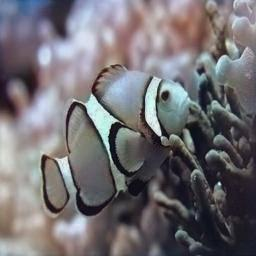
\includegraphics[width = 0.10\linewidth,height=0.10\linewidth]{figures/ch3/compare/EUVP/Ushape/264298_00035269.jpg} & \hspace{-0.40cm}         
			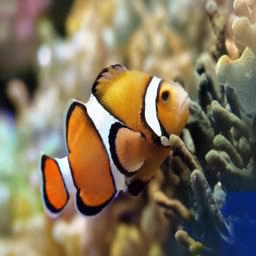
\includegraphics[width = 0.10\linewidth,height=0.10\linewidth]{figures/ch3/compare/EUVP/Ours/264298_00035269.png}   \\

            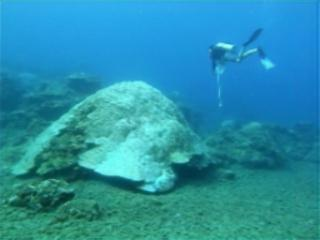
\includegraphics[width = 0.10\linewidth,height=0.10\linewidth]{figures/ch3/compare/EUVP/Input/im_f149_.jpg}  & \hspace{-0.40cm}
			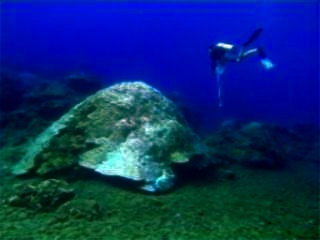
\includegraphics[width = 0.10\linewidth,height=0.10\linewidth]{figures/ch3/compare/EUVP/UDCP/im_f149_.jpg}   & \hspace{-0.40cm}
			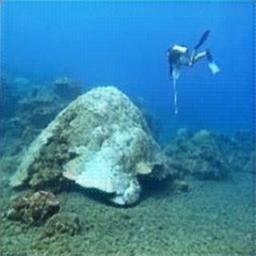
\includegraphics[width = 0.10\linewidth,height=0.10\linewidth]{figures/ch3/compare/EUVP/UGAN/im_f149_.jpg}   & \hspace{-0.40cm}
			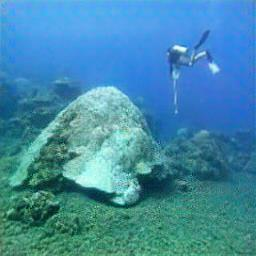
\includegraphics[width = 0.10\linewidth,height=0.10\linewidth]{figures/ch3/compare/EUVP/FGAN/im_f149_.jpg}   & \hspace{-0.40cm}
			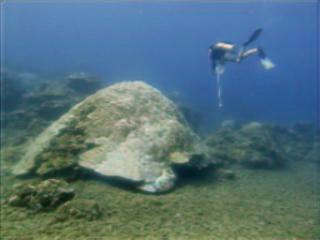
\includegraphics[width = 0.10\linewidth,height=0.10\linewidth]{figures/ch3/compare/EUVP/UWCNN/im_f149_.jpg}  & \hspace{-0.40cm}
			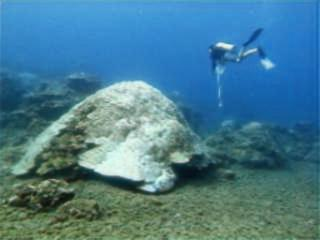
\includegraphics[width = 0.10\linewidth,height=0.10\linewidth]{figures/ch3/compare/EUVP/Ucolor/im_f149_.jpg} & \hspace{-0.40cm}
			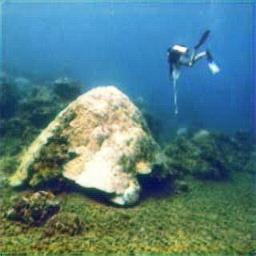
\includegraphics[width = 0.10\linewidth,height=0.10\linewidth]{figures/ch3/compare/EUVP/STSC/im_f149_.jpg}   & \hspace{-0.40cm}
			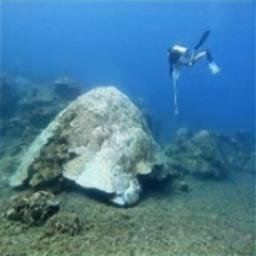
\includegraphics[width = 0.10\linewidth,height=0.10\linewidth]{figures/ch3/compare/EUVP/Ushape/im_f149_.jpg} & \hspace{-0.40cm}  
			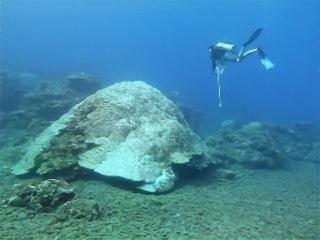
\includegraphics[width = 0.10\linewidth,height=0.10\linewidth]{figures/ch3/compare/EUVP/Ours/im_f149_.png}   
            \\
			\scriptsize Input
			&\hspace{-0.50cm} \scriptsize UDCP\cite{udcp}
			&\hspace{-0.50cm} \scriptsize UGAN\cite{ugan}
			&\hspace{-0.50cm} \scriptsize FGAN\cite{funie_gan}
			&\hspace{-0.50cm} \scriptsize UWCNN\cite{uwcnn}
			&\hspace{-0.50cm} \scriptsize Ucolor\cite{ucolor}
			&\hspace{-0.50cm} \scriptsize STSC\cite{stsc}
			&\hspace{-0.50cm} \scriptsize U-shape\cite{u-shape}
			&\hspace{-0.50cm} \scriptsize Ours
			\\

		\end{tabular}
	\end{center}
	\vspace{-0.4mm}
	\caption{\label{img:visual-euvp}EUVP 数据集上的主观结果比较。在大多数情况下,本章的方法相比其他方法能够更好地恢复物体的颜色,提升画面色彩和对比度。}
	\vspace{-0.3mm}
\end{figure} 

\begin{figure*}[t]
    \vspace{-1mm}
\begin{center}
    \begin{tabular}{ccccccccc}
        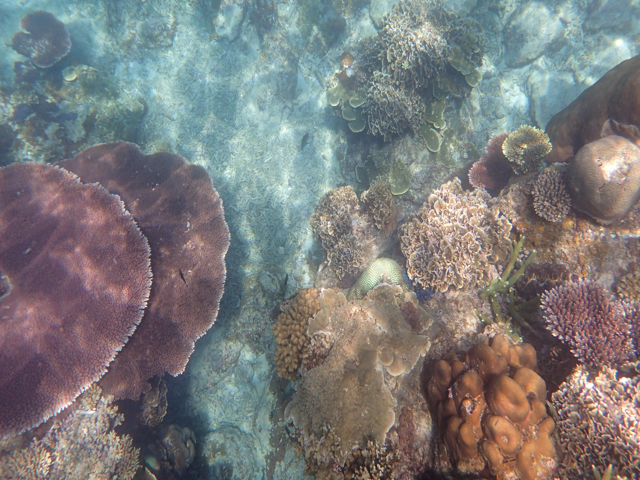
\includegraphics[width = 0.10\linewidth,height=0.10\linewidth]{figures/ch3/compare/UIEB/Input/161_img_.png} & \hspace{-0.40cm}
        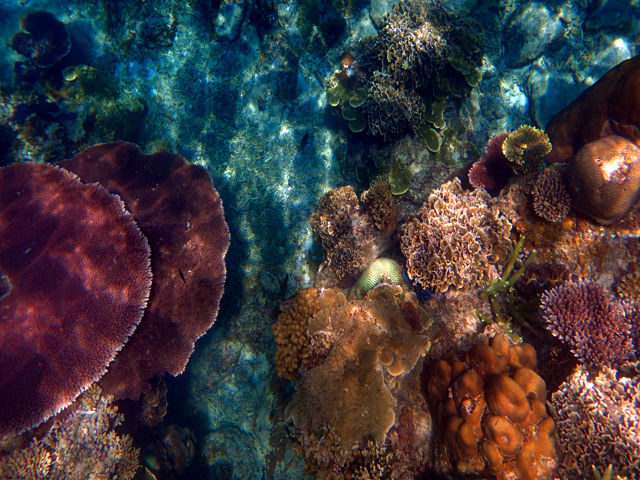
\includegraphics[width = 0.10\linewidth,height=0.10\linewidth]{figures/ch3/compare/UIEB/UDCP/161_img_.png}  & \hspace{-0.40cm}
        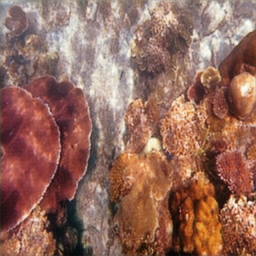
\includegraphics[width = 0.10\linewidth,height=0.10\linewidth]{figures/ch3/compare/UIEB/UGAN/161_img_.png}  & \hspace{-0.40cm}
        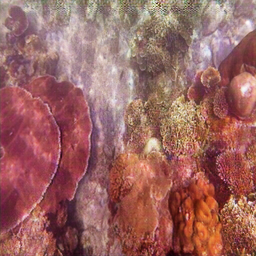
\includegraphics[width = 0.10\linewidth,height=0.10\linewidth]{figures/ch3/compare/UIEB/FGAN/161_img_.png}  & \hspace{-0.40cm}
        \includegraphics[width = 0.10\linewidth,height=0.10\linewidth]{figures/ch3/compare/UIEB/UWCNN/161_img_.png} & \hspace{-0.40cm}
        \includegraphics[width = 0.10\linewidth,height=0.10\linewidth]{figures/ch3/compare/UIEB/Ucolor/161_img_.png}& \hspace{-0.40cm}
        \includegraphics[width = 0.10\linewidth,height=0.10\linewidth]{figures/ch3/compare/UIEB/STSC/161_img_.png}  & \hspace{-0.40cm}
        \includegraphics[width = 0.10\linewidth,height=0.10\linewidth]{figures/ch3/compare/UIEB/Ushape/161_img_.png}& \hspace{-0.40cm} 
        \includegraphics[width = 0.10\linewidth,height=0.10\linewidth]{figures/ch3/compare/UIEB/Ours/161_img_.png}  \\

        \includegraphics[width = 0.10\linewidth,height=0.10\linewidth]{figures/ch3/compare/UIEB/Input/41_img_.png} & \hspace{-0.40cm}
        \includegraphics[width = 0.10\linewidth,height=0.10\linewidth]{figures/ch3/compare/UIEB/UDCP/41_img_.png}  & \hspace{-0.40cm}
        \includegraphics[width = 0.10\linewidth,height=0.10\linewidth]{figures/ch3/compare/UIEB/UGAN/41_img_.png}  & \hspace{-0.40cm}
        \includegraphics[width = 0.10\linewidth,height=0.10\linewidth]{figures/ch3/compare/UIEB/FGAN/41_img_.png}  & \hspace{-0.40cm}
        \includegraphics[width = 0.10\linewidth,height=0.10\linewidth]{figures/ch3/compare/UIEB/UWCNN/41_img_.png} & \hspace{-0.40cm}
        \includegraphics[width = 0.10\linewidth,height=0.10\linewidth]{figures/ch3/compare/UIEB/Ucolor/41_img_.png}& \hspace{-0.40cm}
        \includegraphics[width = 0.10\linewidth,height=0.10\linewidth]{figures/ch3/compare/UIEB/STSC/41_img_.png}  & \hspace{-0.40cm}
        \includegraphics[width = 0.10\linewidth,height=0.10\linewidth]{figures/ch3/compare/UIEB/Ushape/41_img_.png}& \hspace{-0.40cm} 
        \includegraphics[width = 0.10\linewidth,height=0.10\linewidth]{figures/ch3/compare/UIEB/Ours/41_img_.png} 
        \\
        \scriptsize Input
        & \hspace{-0.51cm} \scriptsize UDCP\cite{udcp}
        & \hspace{-0.51cm} \scriptsize UGAN*\cite{ugan}
        & \hspace{-0.51cm} \scriptsize FGAN*\cite{funie_gan}
        & \hspace{-0.51cm} \scriptsize UWCNN\cite{uwcnn}
        & \hspace{-0.51cm} \scriptsize Ucolor\cite{ucolor}
        & \hspace{-0.51cm} \scriptsize STSC*\cite{stsc}
        & \hspace{-0.51cm} \scriptsize U-shape*\cite{u-shape}
        & \hspace{-0.51cm} \scriptsize Ours
        \\
    \end{tabular}
\end{center}
\vspace{-1mm}
\caption{\label{img:visual-uieb}UIEB 数据集上的主观结果比较。本章的方法在高分辨率图像上依旧保持良好的色彩校正能力。(标注为 “*” 的方法限制图像分辨率为 $256 \times 256$)。}
\vspace{-1mm}
\end{figure*}

实验进一步分析了不同方法在高分辨率图像上的增强效果(如图 \ref{img:visual-detail} 所示),
与需要对图像进行压缩处理的方法(FGAN\cite{funie_gan}、UGAN\cite{ugan}、U-shape\cite{u-shape} 和 STSC\cite{stsc})对比,
本章提出的水下图像增强方法可以在不损失图像细节的情况下对任意分辨率的水下图像进行有效增强,在保留物体表面的细节纹理的同时增强色彩和对比度。

\begin{figure}[ht]
	\begin{center}
        \includegraphics[width=0.96\linewidth]{figures/ch3/compare/discussion/res_detail.jpg}
		\\
        \setlength{\tabcolsep}{0pt} % 默认通常是6pt
        \begin{tabular}{
            >{\centering\arraybackslash}p{0.16\linewidth}
            >{\centering\arraybackslash}p{0.16\linewidth}
            >{\centering\arraybackslash}p{0.16\linewidth}
            >{\centering\arraybackslash}p{0.16\linewidth}
            >{\centering\arraybackslash}p{0.16\linewidth}
            >{\centering\arraybackslash}p{0.16\linewidth}
        }
            \footnotesize Input \hspace{-1.5cm}
			& \footnotesize FGAN\cite{funie_gan} 
			& \footnotesize UGAN\cite{ugan} 
			& \footnotesize STSC\cite{stsc} 
			& \footnotesize U-shape\cite{u-shape} 
			& \footnotesize Ours
            \\ 
		\end{tabular}
	\end{center}
	\caption{ \label{img:visual-detail}UIEB 数据集中不同分辨率图像的增强结果比较。对于存在输入大小限制的四种模型使用线性插值来调整其结果的图像分辨率。}
	\vspace{-2mm}
\end{figure}

% \begin{figure}[ht]
% 	\begin{center}
% 		\begin{tabular}{c c c c c c}
% 			\includegraphics[width = 0.15\linewidth]{figures/ch3/compare/resolution/input/2_img__merged.png} & \hspace{-0.50cm}
% 			\includegraphics[width = 0.15\linewidth]{figures/ch3/compare/resolution/FGAN/2_img__resize_merged.png}  & \hspace{-0.50cm}
% 			\includegraphics[width = 0.15\linewidth]{figures/ch3/compare/resolution/UGAN/2_img__resize_merged.png}  & \hspace{-0.50cm}
% 			\includegraphics[width = 0.15\linewidth]{figures/ch3/compare/resolution/STSC/2_img__resize_merged.png}  & \hspace{-0.50cm}
%             \includegraphics[width = 0.15\linewidth]{figures/ch3/compare/resolution/Ushape/2_img__resize_merged.png}  & \hspace{-0.50cm}
% 			\includegraphics[width = 0.15\linewidth]{figures/ch3/compare/resolution/ours/2_img__merged.png}  \\

%             \includegraphics[width = 0.15\linewidth]{figures/ch3/compare/resolution/input/19_img__merged.png} & \hspace{-0.50cm}
% 			\includegraphics[width = 0.15\linewidth]{figures/ch3/compare/resolution/FGAN/19_img__resize_merged.png}  & \hspace{-0.50cm}
% 			\includegraphics[width = 0.15\linewidth]{figures/ch3/compare/resolution/UGAN/19_img__resize_merged.png}  & \hspace{-0.50cm}
% 			\includegraphics[width = 0.15\linewidth]{figures/ch3/compare/resolution/STSC/19_img__resize_merged.png}  & \hspace{-0.50cm}
%             \includegraphics[width = 0.15\linewidth]{figures/ch3/compare/resolution/Ushape/19_img__resize_merged.png}  & \hspace{-0.50cm}
% 			\includegraphics[width = 0.15\linewidth]{figures/ch3/compare/resolution/ours/19_img__merged.png}  \\

%             \includegraphics[width = 0.15\linewidth]{figures/ch3/compare/resolution/input/129_img__merged.png} & \hspace{-0.50cm}
% 			\includegraphics[width = 0.15\linewidth]{figures/ch3/compare/resolution/FGAN/129_img__resize_merged.png}  & \hspace{-0.50cm}
% 			\includegraphics[width = 0.15\linewidth]{figures/ch3/compare/resolution/UGAN/129_img__resize_merged.png}  & \hspace{-0.50cm}
% 			\includegraphics[width = 0.15\linewidth]{figures/ch3/compare/resolution/STSC/129_img__resize_merged.png}  & \hspace{-0.50cm}
%             \includegraphics[width = 0.15\linewidth]{figures/ch3/compare/resolution/Ushape/129_img__resize_merged.png}  & \hspace{-0.50cm}
% 			\includegraphics[width = 0.15\linewidth]{figures/ch3/compare/resolution/ours/129_img__merged.png}  \\

%             \includegraphics[width = 0.15\linewidth]{figures/ch3/compare/resolution/input/17_img__merged.png} & \hspace{-0.50cm}
% 			\includegraphics[width = 0.15\linewidth]{figures/ch3/compare/resolution/FGAN/17_img__resize_merged.png}  & \hspace{-0.50cm}
% 			\includegraphics[width = 0.15\linewidth]{figures/ch3/compare/resolution/UGAN/17_img__resize_merged.png}  & \hspace{-0.50cm}
% 			\includegraphics[width = 0.15\linewidth]{figures/ch3/compare/resolution/STSC/17_img__resize_merged.png}  & \hspace{-0.50cm}
%             \includegraphics[width = 0.15\linewidth]{figures/ch3/compare/resolution/Ushape/17_img__resize_merged.png}  & \hspace{-0.50cm}
% 			\includegraphics[width = 0.15\linewidth]{figures/ch3/compare/resolution/ours/17_img__merged.png}  
%             \\  
% 			\footnotesize Input
% 			& \hspace{-0.36cm} \footnotesize FGAN\cite{funie_gan}
% 			& \hspace{-0.36cm} \footnotesize UGAN\cite{ugan}
% 			& \hspace{-0.36cm} \footnotesize STSC\cite{stsc}
% 			& \hspace{-0.36cm} \footnotesize U-shape\cite{u-shape}
%             & \hspace{-0.36cm} \footnotesize Ours
% 			\\
% 		\end{tabular}
% 	\end{center}
% 	\vspace{-3mm}
% 	\caption{ \label{img:visual-detail}The detailed comparison of enhancement results of four images from the UIEB datasets at different resolutions. We use linear interpolation to resize the image resolution of the results obtained from the other four models.}
% 	\vspace{-3mm}
% \end{figure} 


\subsection{结果讨论}
\subsubsection{水下语义恢复}
为了验证本章提出的水下图像增强算法在减轻水下环境对语义干扰上的有效性,
采用显著性区域检测网络 \cite{sod} 实验对比了原始退化图像与增强后图像的显著性区域检测结果。
如图 \ref{img:sod} 所示,本章的水下图像增强方法显著提升了水下图像的语义信息,
使得原本模糊或难以分辨的显著性区域在增强后的图像中得到了更清晰的表达,
说明增强后的图像能够更好地支持如目标检测和语义分割等图像处理的下游任务,
\begin{figure}[ht]
	\begin{center}
		\begin{tabular}{ccccccccc}
            \vspace{-0.5mm}  
            \raisebox{0.8cm}{\footnotesize Input}   & \hspace{-0.36cm}
            \includegraphics[width = 0.10\linewidth, height=0.10\linewidth]{figures/ch3/compare/discussion/SOD/original/1.JPEG} & \hspace{-0.43cm} 
            \includegraphics[width = 0.10\linewidth, height=0.10\linewidth]{figures/ch3/compare/discussion/SOD/original/2.JPEG}  & \hspace{-0.43cm} 
            \includegraphics[width = 0.10\linewidth, height=0.10\linewidth]{figures/ch3/compare/discussion/SOD/original/3.jpg}  & \hspace{-0.43cm}  
            \includegraphics[width = 0.10\linewidth, height=0.10\linewidth]{figures/ch3/compare/discussion/SOD/original/4.jpg}  & \hspace{-0.43cm} 
            \includegraphics[width = 0.10\linewidth, height=0.10\linewidth]{figures/ch3/compare/discussion/SOD/original/5.JPEG}  & \hspace{-0.43cm} 
            \includegraphics[width = 0.10\linewidth, height=0.10\linewidth]{figures/ch3/compare/discussion/SOD/original/6.jpg}  & \hspace{-0.43cm}
            \includegraphics[width = 0.10\linewidth, height=0.10\linewidth]{figures/ch3/compare/discussion/SOD/original/7.JPEG}  & \hspace{-0.43cm}
            \includegraphics[width = 0.10\linewidth, height=0.10\linewidth]{figures/ch3/compare/discussion/SOD/original/9.jpg} \\
            
            \vspace{-0.5mm} 
            \raisebox{0.8cm}{\footnotesize SOD}   & \hspace{-0.36cm}
            \includegraphics[width = 0.10\linewidth, height=0.10\linewidth]{figures/ch3/compare/discussion/SOD/sod/1.JPEG} & \hspace{-0.43cm}
            \includegraphics[width = 0.10\linewidth, height=0.10\linewidth]{figures/ch3/compare/discussion/SOD/sod/2.JPEG}  & \hspace{-0.43cm}
            \includegraphics[width = 0.10\linewidth, height=0.10\linewidth]{figures/ch3/compare/discussion/SOD/sod/3.jpg}  & \hspace{-0.43cm}
            \includegraphics[width = 0.10\linewidth, height=0.10\linewidth]{figures/ch3/compare/discussion/SOD/sod/4.jpg}  & \hspace{-0.43cm}
            \includegraphics[width = 0.10\linewidth, height=0.10\linewidth]{figures/ch3/compare/discussion/SOD/sod/5.JPEG}  & \hspace{-0.43cm}
            \includegraphics[width = 0.10\linewidth, height=0.10\linewidth]{figures/ch3/compare/discussion/SOD/sod/6.jpg}  & \hspace{-0.43cm}
            \includegraphics[width = 0.10\linewidth, height=0.10\linewidth]{figures/ch3/compare/discussion/SOD/sod/7.JPEG}  & \hspace{-0.43cm}
            \includegraphics[width = 0.10\linewidth, height=0.10\linewidth]{figures/ch3/compare/discussion/SOD/sod/9.jpg}  \\
            
            \vspace{-0.5mm} 
            \raisebox{0.8cm}{\footnotesize Output} & \hspace{-0.36cm}
            \includegraphics[width = 0.10\linewidth, height=0.10\linewidth]{figures/ch3/compare/discussion/SOD/output/1.png} & \hspace{-0.43cm}
            \includegraphics[width = 0.10\linewidth, height=0.10\linewidth]{figures/ch3/compare/discussion/SOD/output/2.png}  & \hspace{-0.43cm}
            \includegraphics[width = 0.10\linewidth, height=0.10\linewidth]{figures/ch3/compare/discussion/SOD/output/3.png}  & \hspace{-0.43cm}
            \includegraphics[width = 0.10\linewidth, height=0.10\linewidth]{figures/ch3/compare/discussion/SOD/output/4.png}  & \hspace{-0.43cm}
            \includegraphics[width = 0.10\linewidth, height=0.10\linewidth]{figures/ch3/compare/discussion/SOD/output/5.png}  & \hspace{-0.43cm}
            \includegraphics[width = 0.10\linewidth, height=0.10\linewidth]{figures/ch3/compare/discussion/SOD/output/6.png}  & \hspace{-0.43cm}
            \includegraphics[width = 0.10\linewidth, height=0.10\linewidth]{figures/ch3/compare/discussion/SOD/output/7.png}  & \hspace{-0.43cm}
            \includegraphics[width = 0.10\linewidth, height=0.10\linewidth]{figures/ch3/compare/discussion/SOD/output/9.png} \\
            
            \vspace{-0.5mm} 
            \raisebox{0.8cm}{\footnotesize SOD} & \hspace{-0.36cm} 
            \includegraphics[width = 0.10\linewidth, height=0.10\linewidth]{figures/ch3/compare/discussion/SOD/sod/1.png} & \hspace{-0.43cm}
            \includegraphics[width = 0.10\linewidth, height=0.10\linewidth]{figures/ch3/compare/discussion/SOD/sod/2.png}  & \hspace{-0.43cm}
            \includegraphics[width = 0.10\linewidth, height=0.10\linewidth]{figures/ch3/compare/discussion/SOD/sod/3.png}  & \hspace{-0.43cm}
            \includegraphics[width = 0.10\linewidth, height=0.10\linewidth]{figures/ch3/compare/discussion/SOD/sod/4.png}  & \hspace{-0.43cm}
            \includegraphics[width = 0.10\linewidth, height=0.10\linewidth]{figures/ch3/compare/discussion/SOD/sod/5.png}  & \hspace{-0.43cm}
            \includegraphics[width = 0.10\linewidth, height=0.10\linewidth]{figures/ch3/compare/discussion/SOD/sod/6.png}  & \hspace{-0.43cm}
            \includegraphics[width = 0.10\linewidth, height=0.10\linewidth]{figures/ch3/compare/discussion/SOD/sod/7.png}  & \hspace{-0.43cm}
            \includegraphics[width = 0.10\linewidth, height=0.10\linewidth]{figures/ch3/compare/discussion/SOD/sod/9.png}  \\
		\end{tabular}
	\end{center}
	\caption{\label{img:sod}原始图像与增强后的图像在显著性区域检测任务中的比较。增强后图像的显著区域边界更加清晰,语义更完整。}
	\vspace{-2mm}
\end{figure}     % sod

\subsubsection{网络架构讨论}
为了探讨网络架构对模型性能的影响,本章对不同网络组件进行了消融实验(如表 \ref{tab:ablation} 所示)。
实验重点分析了时间步嵌入与残差注意力模块对模型的增强效果及其在性能与效率间的权衡。
结果表明,在编码器-解码器的残差模块中去除时间步嵌入(w/o timestep)会明显降低模型对采样时间步的敏感性,从而无法更准确地识别扩散过程中的动态变化。
在所有层中引入残差注意力模块(w/ all layer attention)可以较大的提升模型的特征提取能力,但运行时间显著增加至 1022.20 ms。
相比之下,仅在一层中加入残差注意力模块(w/ one layer attention)时,尽管 PSNR 和 SSIM 稍有下降(分别为 29.90 和 0.91),但运行时间显著降低至 889.32 ms。
为了平衡性能和效率,可以仅在特征分辨率为 $16 \times 16$ 的特定层中引入残差注意力模块(如图\ref{img:network}所示),既能保持较高的效果,又能降低一定的推理时间。
\begin{table}[ht]
    \vspace{-0.4mm}
    \centering
    \caption{\label{tab:ablation}消融实验结果。}
    \setlength{\tabcolsep}{2.6mm}{
        \begin{tabular}{lcccc}
            \toprule
            \specialrule{0em}{1pt}{1pt}
            \textbf{}  & \textbf{PSNR}  & \textbf{SSIM} & \textbf{UIQM} & \textbf{Runtime (ms)} \\
            \hline
            \specialrule{0em}{1pt}{1pt}
            w/o timestep & $21.75$  & $0.84$  & $3.00$ & $\textcolor{red}{\textbf{739.20}}$\\
            \specialrule{0em}{1pt}{1pt}
            w/ all layer attention & $\textcolor{red}{\textbf{31.02}}$  & $\textcolor{red}{\textbf{0.92}}$  & $\textcolor{red}{\textbf{3.05}}$ & $1022.20$\\
            \specialrule{0em}{1pt}{1pt}
            w/ one layer attention & $29.90$  & $0.91$  & $3.04$ & $889.32$\\
            \bottomrule
    \end{tabular}}
    \vspace{1mm}
\end{table}

\subsubsection{步长与采样步数的均衡}
本章最后进一步探讨了滑动窗口步长 ($stride$) 和采样步数 ($S$) 对生成图像效果的影响,以探讨如何在生成质量与效率之间取得最佳平衡。
如图\ref{img:stride-S}(a)所示,当滑动窗口步长等于补丁大小($stride=64$)时,补丁之间完全独立生成,导致过渡区域出现不自然的拼接问题;
当滑动窗口步长略小于补丁大小(如 $stride=48$ 或 $stride=32$)时,补丁之间有适当重叠,重叠区域通过均值采样实现自然的像素过渡,从而生成更平滑、无明显伪影的图像;
进一步减小滑动窗口步长(如 $stride=16$)时,生成结果无明显提升,但其计算复杂度会对应增加。

在基于去噪扩散隐式模型的采样过程中,适当减少采样步数 $S$ 能够显著加速反向去噪过程,但也会对最终生成结果产生负面影响。
如图 \ref{img:stride-S}(b) 所示,采样步数过小(如 $S=2$)时,生成图像的质量明显下降,伪影显著;
当 $S$ 增加至 10 或 15 时,生成效果显著提升,接近最优结果。
进一步增加 $S$(如 $S=20$)时,生成质量提升趋于饱和,说明适当的采样步数已足够实现高质量图像生成。
\begin{figure}[ht]
    \begin{center}
        \begin{tabular}{ccccccc}
            \multicolumn{1}{c}{(a)} & \hspace{-0.46cm}
            \includegraphics[width=0.15\linewidth]{figures/ch3/compare/discussion/input/im_f545_.jpg} & \hspace{-0.46cm}
            \includegraphics[width=0.15\linewidth]{figures/ch3/compare/discussion/diff_stride/stride64/im_f545_.png} & \hspace{-0.46cm}
            \includegraphics[width=0.15\linewidth]{figures/ch3/compare/discussion/diff_stride/stride52/im_f545_.png} & \hspace{-0.46cm}
            \includegraphics[width=0.15\linewidth]{figures/ch3/compare/discussion/diff_stride/stride48/im_f545_.png} & \hspace{-0.46cm}
            \includegraphics[width=0.15\linewidth]{figures/ch3/compare/discussion/diff_stride/stride32/im_f545_.png} & \hspace{-0.46cm}
            \includegraphics[width=0.15\linewidth]{figures/ch3/compare/discussion/diff_stride/stride16/im_f545_.png} \\
            \multicolumn{1}{c}{} & \small Input & \hspace{-0.36cm} \small $stride=64$ & \hspace{-0.36cm} \small $stride=52$ & \hspace{-0.36cm} \small $stride=48$ & \hspace{-0.36cm} \small $stride=32$ & \hspace{-0.36cm} \small $stride=16$ \\
        \end{tabular} 
        \vspace{5mm}
        \begin{tabular}{ccccccc}
            \multicolumn{1}{c}{(b)} &  \hspace{-0.46cm}
            \includegraphics[width=0.15\linewidth]{figures/ch3/compare/discussion/input/im_f565_.jpg} & \hspace{-0.46cm}
            \includegraphics[width=0.15\linewidth]{figures/ch3/compare/discussion/diff_s/s2/im_f565_.png} & \hspace{-0.46cm}
            \includegraphics[width=0.15\linewidth]{figures/ch3/compare/discussion/diff_s/s5/im_f565_.png} & \hspace{-0.46cm}
            \includegraphics[width=0.15\linewidth]{figures/ch3/compare/discussion/diff_s/s10/im_f565_.png} & \hspace{-0.46cm}
            \includegraphics[width=0.15\linewidth]{figures/ch3/compare/discussion/diff_s/s15/im_f565_.png} & \hspace{-0.46cm}
            \includegraphics[width=0.15\linewidth]{figures/ch3/compare/discussion/diff_s/s20/im_f565_.png} \\
            
            \multicolumn{1}{c}{} & \small Input & \hspace{-0.36cm} \small $S=2$ & \hspace{-0.36cm} \small $S=5$ & \hspace{-0.36cm} \small $S=10$ & \hspace{-0.36cm} \small $S=15$ & \hspace{-0.36cm} \small $S=20$ \\
        \end{tabular}
    \end{center}
    \vspace{-6mm}
    \caption{\label{img:stride-S} 不同步长$stride$ 和 采样步数$S$ 的结果。}
    \vspace{-4mm}
\end{figure}

为了进一步验证步长与采样步数的均衡关系,本章在 RUIE \cite{RUIE} 数据集上进行了参数交叉对比实验。
如图 \ref{img:param} 所示,即便采样步数 $S$ 较小或滑动窗口步长$stride$较大,在某些组合下依然能获得良好的增强效果。
这说明较小的步长使得更多的重叠区域参与信息交互与计算,使得能够在较少的采样步数下获得令人满意的结果。
\begin{figure}[t]
    \centering
    \includegraphics[width=0.98\linewidth]{figures/ch3/compare/discussion/param.pdf}
    \caption{\label{img:param}不同步长$stride$和采样步数$S$参数组合下的的增强效果。}
\end{figure}

\section{本章小结}
本章提出了一种基于扩散模型的水下图像增强方法,通过引入时间步嵌入和残差注意力模块,显著提升了模型的特征提取能力。
同时,本章通过实验验证了步长与采样步数的均衡关系,为实际应用中的参数选择提供了参考。
实验结果表明,本章提出的方法在主观视觉效果和客观指标上均表现出色,能够有效提升水下图像的视觉效果和语义信息。



% !TeX root = ../main.tex

\chapter{基于3D高斯泼溅的水下三维重建}
3D 高斯泼溅(3DGS)\cite{3DGS} 已逐步取代神经辐射场(NeRF)\cite{nerf} 技术,成为场景重建领域的热门工具。
3DGS 通过其独特的高斯表示方法,能够在复杂的三维环境中提供更为精确的场景重建能力。与传统的 NeRF 方法相比,3DGS 在处理动态场景时表现出更高的灵活性和适应性。
然而,目前尚缺乏针对水下环境的充分验证与应用研究,主要原因在于缺少专门用于此类任务的水下场景数据集支持。
此外,水下图像存在固有的退化效应(如光散射、色偏)及水流造成的动态扰动,对水下三位重建任务的鲁棒性提出了更高的要求。
图像退化问题可以通过前一章中提出的图像恢复算法进行原始采集图像的质量增强,从而缓解劣质图形在三维重建时对相机位姿估计、点云生成等数据预处理的影响。
但是水下场景中存在的水流造成的动态扰动,需要一种能够有效抑制动态干扰的重建方法。
得益于神经网络的时空预测能力,3DGS 在动态场景的重建中也具备高质量的场景复现能力,
为此,本章提出了一种基于 3DGS 和 KAN \cite{kan}变形机制的水下场景感知增强框架。
该框架旨在通过多阶段的训练模式寻找出特定时刻下的静态场景表示,从而抑制运动干扰并且保留水下场景的基础静态特征。
同时,本章构建了一个专门面向水下场景重建的数据集,并在此数据集上对方法有效性进行验证。
实验结果表明,与其他基准方法相比,本章提出的框架在水下动态场景重建的准确性和鲁棒性方面具有显著优势。

\section{水下动态场景的3D高斯泼溅方法} \label{sec:4dgs}
由于水流造成的动态扰动,场景中的同一物体在不同时间的多帧图像中会表现不同的外观特征以及位置,这会导致重建结果中出现模糊和重影现象。
3D 高斯泼溅方法可以直接对场景信息进行显式表示,这为动态场景建模提供了一种灵活的解决方案,
其核心思想是通过变形每个时间点的 3D 高斯表示,寻找符合动态场景重建的最优变形方法。
通过这种方法,可以在动态场景中更好地捕捉物体的运动轨迹和形变特征。
目前,利用神经网络学习位置与时间信息的映射关系已成为主流方案。
在此基础上,本章重新设计了基于时空信息编码与特征解码的4D高斯泼溅\cite{4DGS}框架,
如图\ref{img:4dgs}所示,该框架通过时空结构编码器高效提取 3D 高斯的时空特征,并结合特征解码器实现高斯变形预测,从而完成水下动态场景的重建,
能够在动态场景中实现高精度的重建效果,尤其是在处理复杂的水下环境时,能够有效应对光线变化和水流扰动带来的挑战。
\begin{figure}[ht]
    \centering
    \includegraphics[width=0.99\textwidth]{figures/ch4/4dgs.pdf}
    \vspace{4mm}
    \caption{基于 3D 高斯泼溅的水下动态场景重建框架}
    \label{img:4dgs}
    \vspace{4mm}
\end{figure}

\subsection{3D高斯时空编码器}
对于一个大小为$H, W, L$的三维网格空间来说,其空间复杂度呈正相关关系。
较高的空间分辨率可以保证最终重建结果的细节质量,但会导致该时空网格的内存占用无法承受。
为了解决这个问题,本章提出了一种基于HexPlane\cite{hex_plane}的时空结构编码器,可以有效减少空间网格的内存占用,避免维度爆炸。

动态场景中的相邻 3D 高斯通常具有显著的时空信息相似性,
特别是在受到单一方向的水流扰动时,这些相邻 3D 高斯在时间维度上表现出的相似性特征尤为明显。
HexPlane 模块可以有效利用这种相邻时空信息的相似性质,对高维时空信息进行特征分解,从而优化内存占用并降低计算复杂度。
基于 HexPlane 特征分解模块,本章设计了一种高效的时空结构编码器 $\mathcal{H}$,
该编码器由多个分辨率的二维空间网格特征和一个多层感知机(MLP)模块组成。
其主要目标是结合 3D 高斯的位置与时间信息,将其映射到低维特征空间,为后续多头解码器进行变形预测提供支持。

为了避免高维空间的维度灾难,本章的HexPlane特征分解采用了K-Planes\cite{k-planes}的方法将每个点的特征分解为它在空间中的特征和它在每个轴(XYZ)上关于时间的特征,从而优化内存占用并降低计算复杂度。
具体做法是将原始 4D 神经体素分解为 6 个独立的平面模块,这些模块能够有效表示一定区域内的 3D 高斯,并通过时间维度进一步捕捉高斯变形信息。
因此3D时空结构编码器$\mathcal{H}$包含6个多分辨率平面模块$R_l(i,j)$和一个小型MLP模块$\phi_d$,如公式\ref{eq:encoder_H}所示:
\begin{equation}
\label{eq:encoder_H}
\mathcal{H}(G, t) = \{ R_l(i,j), \phi_d \ | \ (i,j) \in \{(x,y), (x,z), (y,z), (x,t), (y,t), (z,t)\}, l \in \{1, 2\} \}
\end{equation}

其中,$\mathcal{X} = (x, y, z)$表示3D高斯的中心位置,$l$表示上采样的尺度,
$R(i,j)$是每个体素平面模块,维度为$R(i,j) \in \mathbb{R}^{h \times l N_i \times l N_j}$,
其中$h$表示平面中单个网格特征的维度,$N_i,N_j$表示每个平面体素网格的基本分辨率。

为提取每个体素特征,需要在6个2D体素平面中对3D高斯体的信息进行编码,可以使用双线性插值的方法查询平面体素网格四个顶点的特征,计算公式为:
\begin{equation}
f_h = \bigcup_l \prod \text{interp}(R_l(i,j)), \quad (i,j) \in \{(x,y),(x,z),(y,z),(x,t),(y,t),(z,t)\}
\end{equation}

其中,$f_h \in \mathbb{R}^{h \times l}$表示神经体素的特征。
随后,MLP 模块 $\phi_d$ 融合所有特征以生成最终的编码表示:
\begin{equation}
f_d = \phi_d(f_h)
\end{equation}  

该编码过程不仅可以高效捕获动态场景中时空特征的变化,还为后续高斯变形计算奠定基础,在动态场景中更好地捕捉物体的运动轨迹和形变特征,提高重建的精度和稳定性

\subsection{基于KAN的特征解码器}
时空结构编码器生成的 3D 高斯特征随后被输入到多头高斯变形解码器 $\mathcal{D}$ 中,以计算每个 3D 高斯在不同时刻下的变形信息。
该解码器包含多个KAN模块,分别用于估计位置变形$\Delta \mathcal{X}$、旋转变形$\Delta r$和缩放变形$\Delta s$。
这些变形信息构成了变形后的 3D 高斯表示$G^\prime=\{\mathcal{X}^\prime, s^\prime, r^\prime, \sigma, \mathcal{C} \}$。
KAN 模块通过学习神经元的最优激活方式,在保证解码准确性的同时减少了所需的神经元数量。
基于KAN的特征解码器通过自适应的方式预测形变量,最终的变形3D高斯可以表示为:
\begin{equation}
    G^\prime = \{ \mathcal{X} + \Delta \mathcal{X}, r + \Delta r, s + \Delta s, \alpha + \Delta \alpha, \mathcal{C} + \Delta \mathcal{C} \}
\end{equation}

不同时刻下的3D高斯可以有效处理水下环境中的动态特征,生成精准的动态场景重建结果。

\section{水下静态三维场景自对抗训练}
\subsection{多阶段训练模式}
在水下复杂环境中,水流引发的动态干扰会导致场景中物体晃动,使得完全静态的水下场景重建变得极具挑战性。
尽管基于动态场景重建的方法能够在一定程度上保留动态效果并生成高质量、逼真的新视图,
但在单目相机拍摄的水下动态场景中,某些时刻可能出现异常的重建现象。这种现象通常由以下原因导致:
(1)某些时刻运动干扰过于强烈,画面质量显著下降;
(2)动态场景数据集中缺乏足够的视角覆盖,导致 3D 高斯变形预测出现误差。

真实世界中水下重建场景的对象位置相对固定,且水流带来的扰动具有一定周期性,导致不同视角下的场景存在相似的高频信息。
为捕捉这些高频静态特征并实现高质量水下场景重建,本章提出了一种带有场景过滤模块的多阶段训练模式。
如图 \ref{img:3_stage} 所示,该模式分为以下三个阶段:初始化训练阶段、动态场景训练阶段和目标场景训练阶段。
\begin{figure}[htbp]
    \centering
    \includegraphics[width=0.95\textwidth]{figures/ch4/3_stage.pdf}
    \caption{多阶段训练模式}
    \label{img:3_stage}
\end{figure}

(1)初始化训练阶段:利用基于结构化运动(SfM)方法\cite{sfm1}\cite{sfm2}初始化的点云,对 3D 高斯初始表示进行优化。
\begin{equation}
    G_1 = Train_{w/o-\mathcal{F} }(\mathcal{C})
\end{equation}
其中,$G_1$为初始化训练的3D高斯,$\mathcal{C}$为完整的训练相机序列数据,$\mathcal{F}$为基于3D高斯时空编码器与KAN的特征解码器网络。
该阶段旨在快速完成初步重建,缓解动态重建初期的不稳定性,避免后续训练阶段中由于梯度爆炸出现程序崩溃,故暂时不使用变形预测网络$\mathcal{F}$。

(2)动态场景训练阶段:通过章节 \ref{sec:4dgs} 中介绍的 3D 高斯时空编码器与基于 KAN 的特征解码器构成的变形预测网络$\mathcal{F}$进行动态场景的训练,从而提高水下动态重建质量,同时保留动态效果。
\begin{equation}
    G_2, \mathcal{F} = Train_{w/-\mathcal{F} }(\mathcal{C})
\end{equation}
其中,$G_2$为动态场景训练的 3D 初始化高斯,按照$\mathcal{C}$中的不同相机位姿的时间和变相预测网络$\mathcal{F}$对$G_2$的3D高斯进行变形预测,
对变形后的 3D 高斯$G_2^\prime$进行光栅化渲染,利用梯度传播同时优化$G_2$和$\mathcal{F}$。

(3)目标场景训练阶段:首先结合上一阶段优化的变形预测网络$\mathcal{F}$和$G_2$对完整的训练数据$\mathcal{C}$进行筛选,
提取其中的最高频出现的静态场景数据$\mathcal{C}_s$:
\begin{equation}
    \mathcal{C}_s = Filter(G_2, \mathcal{C}, \mathcal{F})
\end{equation}
最后按照新的训练数据$\mathcal{C}_s$进行目标场景训练,从而实现目标静态场景的高质量重建,同时依旧保留 3D 高斯变形机制,以提高重建的鲁棒性。
\begin{equation}
    G_3, \mathcal{F} = Train_{w/-\mathcal{F} }(\mathcal{C}_s)
\end{equation}

通过采用这种多阶段训练模式,利用筛选后的训练数据$\mathcal{C}_s$去除原始数据中的干扰数据,进一步提升了静态场景的重建精度和稳定性。

\subsection{场景过滤模块}
为确保在目标水下静态场景训练阶段能够高效筛选出静态优质片段,本章设计了一种基于时序分析的自适应场景过滤模块。
该模块通过分析场景中3D高斯的时序变化特征,结合多尺度静态片段融合策略,实现了对水下场景静态片段数据的精确提取。
如图\ref{img:filter}所示,该模块包含时序差分分析、自适应阈值分割和多尺度静态片段融合三个关键步骤。
\begin{figure}[htbp]
    \centering
    \includegraphics[width=0.95\textwidth]{figures/ch4/filter.pdf}
    \caption{场景过滤模块}
    \label{img:filter}
\end{figure}

\subsubsection{时序差分分析}
基于4.2.1节中第二阶段训练的3D高斯变形预测网络$\mathcal{F}$,可以得到所有训练数据相机序列$\mathcal{C}$对应时刻$t$下3D高斯位置变形$\mathcal{X}_t=\mathcal{F}(G, t)$,其中$G$为上阶段训练的初始化3D高斯。
接下来对相邻时刻的3D高斯变形进行差分分析,计算每个时间步的场景变化量$\delta_i$。
例如,对于时刻$t_i$和$t_{i+1}$,通过计算变形后高斯位置$\mathcal{X}_i$和$\mathcal{X}_{i+1}$之间的欧氏距离来量化场景变化:
\begin{equation}
\delta_i = \|\mathcal{X}_{i+1} - \mathcal{X}_i\|_2
\end{equation}
统计所有相邻时刻的场景变化量得到时序差分序列$\delta$。

为减少噪声影响,对时序数据采用滑动窗口平滑处理得到的时序差分序列$\delta_s$。
具体做法是,对于每个时刻$i$,通过在其前后$\lfloor\omega/2\rfloor$个时刻范围内计算均值来平滑当前时刻的变化量:

\begin{equation}
\delta_s^i = \frac{1}{w_{\text{end}} - w_{\text{start}} + 1} \sum_{j=w_{\text{start}}}^{w_{\text{end}}} \delta_j
\end{equation}

其中,$w_{\text{start}} = \max(1, i - \lfloor\omega/2\rfloor)$和$w_{\text{end}} = \min(|\Delta|, i + \lfloor\omega/2\rfloor)$分别表示滑动窗口的起始和结束位置。
这种自适应窗口边界的处理方式确保了序列首尾处的平滑操作也能得到合理的结果。最终得到平滑后的时序差分序列$\delta_s$。

窗口大小$\omega$的选择需要在平滑效果和时间分辨率之间进行权衡。
较大的窗口尺寸可以更好地抑制噪声,但可能会模糊时间边界,导致相邻静态片段之间的过渡不够清晰;
较小的窗口尺寸能够保持较高的时间分辨率,有利于准确定位场景变化的时间点,但可能会收到本身数据质量的影响。
本章采用窗口大小为5的滑动窗口进行时序差分分析,
该窗口大小能有效平滑数据之间的短期变化,为后续的静态片段提取提供了可靠的基础。

\subsubsection{自适应阈值分割}
本模块采用OTSU自适应阈值算法对平滑后的时序差分序列进行分割。
该算法通过最大化类间方差的方式,自动确定最优分割阈值$\tau_{\text{otsu}}$,常常在图像分割任务中用于分割出前景和背景。具体计算步骤如下:

(1)首先统计出序列$\delta_s$的直方图分布$\mathcal{H}$,将数据范围等分为50个区间,计算每个区间的中心值$x_i$和对应的频数$n_i$;

(2)计算序列的总样本数$N$和全局均值$\mu_T$:
\begin{equation}
N = \sum_{i=1}^{50} n_i, \quad \mu_T = \frac{1}{N}\sum_{i=1}^{50} x_i \cdot n_i
\end{equation}

(3)对每个可能的阈值$\tau$,计算前景类(小于等于阈值)的累积统计量:
\begin{equation}
n_b(\tau) = \sum_{i=1}^{\tau} n_i, \quad \mu_b(\tau) = \sum_{i=1}^{\tau} x_i \cdot n_i
\end{equation}

(4)计算前景类和背景类的类间方差:
\begin{equation}
\sigma_B^2(\tau) = \frac{n_b(\tau)}{N} \cdot \frac{N-n_b(\tau)}{N} \cdot [\frac{\mu_b(\tau)}{n_b(\tau)} - \frac{\mu_T \cdot N-\mu_b(\tau)}{N-n_b(\tau)}]^2
\end{equation}

(5)选择使类间方差最大的阈值作为最优分割阈值:
\begin{equation}
\tau_{\text{otsu}} = \arg\max_{\tau} \{\sigma_B^2(\tau)\}
\end{equation}

这种基于类间方差最大化的阈值选择方法,能够自动找到最优的分割点,将时序差分序列$\delta_s$分为多个静态片段(低于阈值)$\mathcal{S}$和动态片段(高于阈值)两类。

OTSU算法的优势在于其自适应性,无需人工设定固定阈值,能够根据场景的实际变化特征自动调整分割阈值,提高了方法的泛化能力。

\subsubsection{多尺度静态片段融合}
在得到多个静态片段后,还需要对这些片段进行相似性检查,以确保最终的静态片段集合$\mathcal{S}$中只包含具有相似静态场景特征的片段。
该策略不仅考虑了单个静态片段的时间连续性,还通过跨片段的相似性分析,
实现了对具有相似静态特征但在时间上不连续的片段的有效融合:

(1) 首先识别最长的静态片段$\mathcal{S}_{\text{max}}$,并从中随机采样参考数据$\mathcal{R}$。
   最长静态片段通常包含了场景最稳定的部分,因此其特征可以作为评估其他片段的可靠基准;

(2)对其他静态片段$s\in\mathcal{S}$进行验证,计算其采样数据$\mathcal{D}_s$与参考数据$\mathcal{R}$的相似度:
\begin{equation}
\text{sim}(\mathcal{D}_s, \mathcal{R}) = \frac{1}{|\mathcal{D}_s||\mathcal{R}|}\sum_{d \in \mathcal{D}_s}\sum_{r \in \mathcal{R}}\|d - r\|_2
\end{equation}

(3)当相似度满足阈值条件时,将该静态片段加入有效片段集合$\mathcal{S}_{\text{valid}}$:
\begin{equation}
\mathcal{S}_{\text{valid}} = \{s \ | \ \text{sim}(\mathcal{D}_s, \mathcal{R}) < \tau_{\text{otsu}}\}
\end{equation}

最终,通过合并所有有效静态片段,得到用于静态场景重建的相机序列$\mathcal{C}_s=\bigcup_{s\in\mathcal{S}_{\text{valid}}}\mathcal{D}_s$。
该多尺度融合策略不仅保证了静态特征提取的准确性,还提高了算法对水下场景周期性运动的适应能力。
特别地,通过随机采样和相似度比较的方式,该策略能够有效处理由于水流扰动导致的周期性运动,
在保留场景静态结构的同时,避免了过度筛选导致的信息丢失。

\subsection{损失函数设计}
与其他重建方法类似\cite{3DGS}\cite{tineuvox}\cite{dnerf},本文采用L1颜色损失(L1 Color Loss)来监督训练过程,
确保生成的3D高斯在颜色方面与目标场景的实际颜色保持一致。
此外,还引入了基于网格的全变差损失(Total Variation Loss,$\mathcal{L}_{tv}$),
以减少噪声并提高重建结果的平滑性。

L1颜色损失用于衡量生成的场景颜色与真实场景颜色之间的绝对误差,计算公式为:
\begin{equation}
    \mathcal{L}_{color} = \sum_{i} \left\| \hat{C}_i - C_i \right\|_1
\end{equation}

其中,$\hat{C}_i$是模型生成的第$i$个像素的颜色值,$C_i$是对应的真实颜色值。

全变差损失通过度量网格中像素值的梯度变化来减少不必要的细节和噪声,从而增强重建结果的平滑性和稳定性,特别是在处理高频细节和复杂动态场景时。
其计算公式为:
\begin{equation}
    \mathcal{L}_{tv} = \sum_{i,j} \left\| \nabla G(i,j) \right\|_2
\end{equation}

其中,$\nabla G(i,j)$表示网格中位置$(i,j)$的梯度,衡量的是相邻体素之间的变化。这个损失项在训练过程中有助于避免模型过度拟合细节,从而提高重建的鲁棒性。

最终的总损失函数 $\mathcal{L}_{total}$ 结合了上述两种损失,通过加权组合实现颜色一致性与平滑性的平衡:
$$
\mathcal{L}_{total} = \mathcal{L}_{color} + \lambda_{tv} \cdot \mathcal{L}_{tv}
$$

其中,$\lambda_{tv}$是全变差损失的权重系数,用于平衡颜色损失和平滑性损失之间的影响。
通过最小化总损失函数,模型不仅能够实现对动态场景的高精度重建,还能有效抑制噪声的干扰,保证生成结果的平滑性和视觉质量。

\section{实验结果}
\subsection{水下重建数据集}
为验证水下重建方法的有效性,本章制作了一个专用水下重建数据集 3DUW。
首先,搭建了一个可控的人造水下场景,并通过组合不同的环境条件(水流扰动和色偏)生成四组配对数据集,以测试算法在动态扰动抑制和颜色校正(去色偏)能力上的表现。
如图 \ref{img:3DUW} 所示,不同环境条件下的数据集为算法的泛化性能验证提供了丰富的场景样本。
随后,使用单目相机从多个角度和时间点采集水下场景图像,应用SfM算法\cite{sfm1}\cite{sfm2}对数据进行预处理,生成每张图像对应的相机位姿信息和初始点云。
\begin{figure}
    \centering
    \includegraphics[width=0.95\textwidth]{figures/ch4/3DUW.pdf}
    \caption{3DUW 数据集}
    \label{img:3DUW}
\end{figure}

另外,由于3DGS的重建质量在很大程度上依赖于SfM中获得的初始点云。
而水下原始图像由于存在不同程度的模糊和色偏,导致SfM算法难以提取准确的特征点,只会产生稀疏的点云。
为了形成一个更加密集的点云,在获取水下图像后,使用K-Nearest-Neighbor(KNN)算法在现有点的外围添加额外的点。
算法\ref{eq:knn}描述了向原有稀疏点云添加补充点的过程。
\begin{algorithm}[t]
    \caption{\label{eq:knn}添加额外点云}
    \KwIn{$\mathcal{G}$: 从 SfM 计算的点云}
    \KwIn{$K$: 需要查找的邻近点个数}
    \KwIn{$N_p$: 需要生成的额外点个数}
    \KwIn{$t_d$: 新生成点与已有点之间的最小距离要求}
    
    $P_\text{add} \leftarrow \text{GenerateRandomPoints}(\mathcal{P}, N_p)$\tcp*{均匀采样生成 $N_p$ 个新点}
    
    \For{每个 $p \in P_\text{add}$}{
        $\mathcal{P}_\text{knn} \leftarrow \text{FindNearestNeighbors}(\mathcal{P}, p, K)$\tcp*{找到 $p$ 在 $\mathcal{P}$ 中的 $K$ 个最近邻点}
        $\mathcal{P}_\text{valid} \leftarrow \text{CheckDistance}(\mathcal{P}_\text{knn}, p, t_d)$\tcp*{筛选出与 $p$ 距离满足要求的邻居点}
    
        \If{$|\mathcal{P}_\text{valid}| > 0$}{
            $p_c \leftarrow \text{LinearInterpolate}(\mathcal{P}_\text{valid}, p)$\tcp*{线性插值生成新点的颜色}
            $\text{AddToPointCloud}(\mathcal{P}, p, p_c)$\tcp*{将新点添加到点云 $\mathcal{P}$ 中}
        }
    }
\end{algorithm}

首先,通过均匀采样的方法在点云范围内生成$N_p$个随机的新点$P_\text{add}$。对于每个新点$p$,算法利用KNN方法从初始点云中找到其K个最近邻点,构成候选邻域集合$\mathcal{P}_\text{knn}$。
随后,通过检查邻近点与新点之间的距离,通过$t_d$筛选出满足最小距离要求的有效邻居点集合$\mathcal{P}_\text{valid}$。
如果有效邻居点集合非空,算法通过对有效邻居点的颜色信息进行线性插值,估算新点的颜色属性,并将该点及其颜色属性添加到点云中,完成补充点的生成。
这样的操作确保了新增点既满足稠密性需求,又与原始点云保持一致的几何和颜色特性。
该算法通过逐点更新的方式动态扩展了点云密度,同时有效避免了新增点与原始点过度重叠或无效分布的问题,为水下重建提供了更加丰富且高质量的点云数据支撑。

\subsection{实验设置}
为验证本章提出水下三维重建方法的性能和鲁棒性,实验选用了两组真实水下重建数据集:自制的 3DUW 数据集和公开数据集 SeaThru-NeRF\cite{seathru}。
其中3DUW为自制数据集,SeaThru-NeRF包含了三个不同的海洋中潜水获得的多图像水下场景:
以色列埃拉特的红海海域(SeaThru-NeRF-1,29张)、加勒比海库拉索海域(SeaThru-NeRF-2,21张)和太平洋巴拿马运河水域(SeaThru-NeRF-3,18张)。

两组数据集的划分如表 \ref{tab:recondata_split} 所示。
\begin{table}[htbp]
    \centering
    \caption{水下重建数据集划分}
    \label{tab:recondata_split}
    \begin{tabular}{cccc}
        \toprule
        数据集 & 训练集 & 测试集 & 共计 \\
        \midrule
        3DUW-1 & 100 & 50 & 150 \\
        3DUW-2 & 100 & 50 & 150 \\
        3DUW-3 & 100 & 50 & 150 \\
        3DUW-4 & 100 & 50 & 150 \\
        SeaThru-NeRF-1 & 22 & 7 & 29 \\
        SeaThru-NeRF-2 & 15 & 6 & 21 \\
        SeaThru-NeRF-3 & 15 & 3 & 18 \\
        \bottomrule
    \end{tabular}
\end{table}
实验的时空编码器与解码器均基于 PyTorch 框架\cite{pytorch}实现,利用其高效的深度学习工具链保证了模型的开发与训练效率。
所有实验均在单张 RTX 3060 GPU 上完成,批量大小为1,初始化训练、动态场景训练和目标场景训练的迭代次数分别设置为 3000 次、20000 次和 10000 次。

\subsection{定量评价}
为全面评估水下场景重建方法的性能,实验采用除章节\ref{sec:quantitative}中的参考指标PSNR与SSIM外,还引入了感知质量指标以及渲染时的运行帧率。

(1)感知质量指标(LPIPS)\cite{lpips}: 人类可以快速评估两幅图像之间的感知相似性,但是其背后的底层过程非常复杂,涉及对图像不同尺度的特征的比较过程。
因此,LPIPS 提出了使用预训练的深度网络来提取图像特征,然后计算这些特征之间的距离,以评估图像之间的感知相似度;
\begin{equation}
    d(x, x_0) = \sum_{l} \frac{1}{H_l W_l} \sum_{h,w} \left\| w_l \odot (\hat{y}^l_{hw} - \hat{y}^l_{0hw}) \right\|_2^2
\end{equation}

其中,$x$和$x_0$分别表示重建图像和参考图像,$H_l,W_l$表示图像在第$l$个尺度上的特征图的尺寸,$\hat{y}^l_{hw}$和$\hat{y}^l_{0hw}$表示图像在该尺度上的特征图在位置$(h, w)$的值,$w_l$是第$l$个尺度的权重系数。

(2)运行帧率(FPS):使用模型在1s内可以光栅化渲染的图像数量,衡量模型的重建时运行速度。

实验对包括 TiNeuVox\cite{tineuvox}、3DGS\cite{3DGS}、4DGS\cite{4DGS}和 Sea-NeRF\cite{seathru}
在内的多个基线方法进行了比较,实验结果见表 \ref{tab:res_3duw}和\ref{tab:res_seanerf},
由于本章提出的方法会对原始训练数据进行筛选,因此,测试集上的实验仅比较场景过滤模块筛选后的数据,以确保评价的公平性和一致性。

\begin{table} [htbp]
    \small
    \centering
    \caption{不同方法在数据集 3DUW 上的定量结果。}
    \setlength{\tabcolsep}{10pt}
    \begin{tabular}{lcccccc} 
    \toprule
    Model  & PSNR(dB)↑ & SSIM↑ & LPIPS↓ & Time↓ &  FPS ↑  \\
    \midrule  
    Sea-NeRF\cite{seathru} & 21.09& 0.92 & 0.09 & 55 mins & 1.59\\
    3DGS~\cite{3DGS} &22.34 & 0.91 & 0.08 & \textcolor{red}{\textbf{14}} mins  & \textcolor{red}{\textbf{94}}\\
    TiNeuVox~\cite{tineuvox}  & 28.81 & 0.95 &  0.03 & 60 mins & 0.79\\ 
    4DGS\cite{4DGS} & 34.22&\textcolor{red}{\textbf{0.98}} &\textcolor{red}{\textbf{0.02}}& 27 mins&44 \\
    Ours & \textcolor{red}{\textbf{34.58}} & \textcolor{red}{\textbf{0.98}} & \textcolor{red}{\textbf{0.02}} & 38 mins & \textcolor{red}{\textbf{94}}\\
    \bottomrule
    \end{tabular}  
    \label{tab:res_3duw}
\end{table}
    
\begin{table} [htbp]
    \small
    \centering
    \caption{不同方法在数据集 SeaThru-NeRF 上的定量结果。}
    \setlength{\tabcolsep}{10pt}
    \begin{tabular}{lcccccc} 
    \toprule
    Model  & PSNR(dB)↑ & SSIM↑ & LPIPS↓ & Time↓ &  FPS ↑  \\ 
    \midrule  
    Sea-NeRF\cite{seathru} & 32.79 & 0.97 & 0.03 & 53 mins & 1.64\\
    3DGS~\cite{3DGS} &32.84 & 0.93 & 0.08&\textcolor{red}{\textbf{13}} mins  &\textcolor{red}{\textbf{94}}\\
    TiNeuVox~\cite{tineuvox}  & 32.67 & 0.97 &  0.04 & 61 mins & 0.79\\ 
    4DGS\cite{4DGS} & 32.05&\textcolor{red}{\textbf{0.98}} &\textcolor{red}{\textbf{0.02}}& 27 mins&42 \\
    Ours & \textcolor{red}{\textbf{32.90}} & \textcolor{red}{\textbf{0.98}} & \textcolor{red}{\textbf{0.02}} & 40 mins & \textcolor{red}{\textbf{94}}\\
    \bottomrule
    \end{tabular}  
    
    \label{tab:res_seanerf}
\end{table}

从表\ref{tab:res_3duw}可以看出,由于 3DUW 数据集包含一定水下动态场景,TiNeuVox\cite{tineuvox}、4DGS\cite{4DGS}和我们的方法在重建图像的的感知质量评价指标上会明显领先与Sea-NeRF\cite{seathru}和3DGS\cite{3DGS},
这是因为前者都加入了针对动态场景的时序信息,从而可以自适应的调整与参考图像相同的场景变化,最终获得和参考图像更相似的渲染结果,所以在PSNR、SSIM和LPIPS指标上表现更好。
但是由于 SeaThru-NeRF 数据集主要是为了水下静态场景的3D重建而制作,所以在PSNR、SSIM和LPIPS这三种感知质量评价指标上五种方法的表现几乎一致。

另外,从表\ref{tab:res_3duw}和\ref{tab:res_seanerf}可以看出,3DGS\cite{3DGS}在训练耗时上具有最好的表现,
我们的方法和4DGS\cite{4DGS}在训练耗时上表现的差距主要来自于的 3D 高斯变形预测网络中的特征解码器部分,
由于我们采用基于KAN的特征解码器,相比MLP会消耗更多的训练时间。
但是本章的方法在渲染速度上继承了3DGS\cite{3DGS}的优势,这是因为虽然在训练中加入了动态重建模式,
但是实际渲染时,我们开启静态场景的渲染模式,同时可以保证优于3DGS的渲染结果质量。
而Sea-NeRF\cite{seathru}和TiNeuVox\cite{tineuvox}都是基于NeRF的重建方法,这导致其在训练耗时和渲染速度上表现非常糟糕,
说明空间信息的隐式表达在重建水下场景时存在一定的局限性。


\subsection{主观评价}
Sea-NeRF\cite{seathru}数据集三种场景的部分重建结果如图 \ref{img:res_seanerf} 所示,从中可以看出,在该种水下静态数据集上基于NeRF的方法与基于3DGS的方法表现几乎一致。
物体的轮廓较为清晰,画面没有明显的伪影,但是TiNeuVox\cite{tineuvox}和Sea-NeRF\cite{seathru}的重建结果在某些颜色上存在一定对比度不足的问题,本章的方法在对比度的表现上更好。
\begin{figure}[htbp]
    \centering
    \includegraphics[width=0.99\textwidth]{figures/ch4/seanerf-res.pdf}
    \caption{SeaThru-NeRF 数据集水下重建结果对比}
    \label{img:res_seanerf}
\end{figure}

3DUW 数据集的部分重建结果如图 \ref{img:res_3duw} 所示,从中可以看出在具有动态干扰的环境中,
TiNeuVox\cite{tineuvox}、4DGS\cite{4DGS}和本章的方法可以有效适应场景的变化,重建场景中移动的物体可以保持较好的视觉细节,物体边缘清晰。
但是3DGS\cite{3DGS}和Sea-NeRF\cite{seathru}由于没有加入时序信息,在某些时刻和视角下,
其渲染效果不够稳定,特别是对于有位置变化的物体来说,其细节表现较差,模型无法对其进行准确的建模,画面中存在明显的模糊和伪影。


另外,本章的方法通过场景过滤模块能够有效筛选出因水流扰动导致的不利数据,避免了这些数据对其他正常训练数据的视觉细节产生的负面影响。
通过剔除这些不利数据,本文方法成功保留了目标场景的完整性,显著提升了动态场景重建的整体质量。
从结果来看,添加第三阶段的目标场景训练后,最后的渲染结果在对比度上表现相比4DGS\cite{4DGS}有显著的提升。


\begin{figure}[htbp]
    \centering
    \includegraphics[width=0.99\textwidth]{figures/ch4/3duw-res.pdf}
    \caption{3DUW 数据集水下重建结果对比}
    \label{img:res_3duw}
\end{figure}



\subsection{结果讨论}
\subsubsection{消融实验}
为了验证本章所提出的各个模块的有效性,在 3DUW 数据集上进行了消融实验,
主要探究 KAN 在 3D 高斯变形网络的特征解码器中相比 MLP 是否可以带来有效提升,
另外,本章提出利用场景过滤模块筛选出有利数据,通过增加目标场景训练阶段,在保留原有3DGS的渲染速度优势的同时,
提高在水下具有干扰场景下的重建质量,其有效性需要通过实验进行验证。

实验结果如表\ref{tab:recon_ablation}所示,可以看出使用KAN特征解码器相比传统的MLP特征解码器,在 PSNR 定量指标上提升了0.14dB,
证明了KAN特征解码器相比MLP特征解码器在3D高斯变形网络中具有一定的优势。另外,在使用KAN特征解码器的基础上,添加场景过滤模块和目标场景训练阶段后,
在PSNR定量指标上相比简单的双阶段训练提升了0.36dB,在SSIM定量指标上也有0.01的提升,
说明通过场景过滤模块可以有效消除由水流运动引起的噪声干扰数据,保留原始训练数据中的高频静态场景,从而提升目标场景训练阶段的有效性。

\begin{table}
    \centering
    \caption{消融实验结果}
    \label{tab:recon_ablation}
    \begin{tabular}{lcc}
        \toprule
        模型 & PSNR(dB)↑ & SSIM↑ \\
        \midrule
        3DGS + MLP & 34.22 & 0.97 \\
        3DGS + KAN & 34.36 & 0.97\\
        3DGS + KAN + Filter & \textcolor{red}{\textbf{34.58}} & \textcolor{red}{\textbf{0.98}} \\
        \bottomrule
    \end{tabular}
\end{table}


\subsubsection{局限性}
尽管本文方法在 3DUW 数据集中展现了成功重建水下静态目标中心场景的能力,但仍存在以下局限性和挑战:
(1)训练数据覆盖不足:为确保场景过滤模块能够选择足够的训练数据,这对数据集本身提出了必须能够提供足够数量不同时间以及视角图像的需求;
(2)复杂动态场景的挑战:但场景过滤模块只能筛选出动态场景中的高频部分,对于复杂的多物体运动场景仍有一定局限性,无法同时选择多个水下物体的运动中心。

\section{本章小结}
本章提出了一种基于时空编码器和KAN特征解码器的水下三维重建方法。
首先,通过时空编码器提取水下图像的时空特征,并使用KAN特征解码器进行特征解码,生成高维特征。
然后,通过场景过滤模块筛选出有利数据,并使用3DGS\cite{3DGS}的3D高斯变形预测网络预测高斯变形,生成高质量的3D高斯变形场。
最后,通过3D高斯变形场生成高质量的3D高斯变形场。



% !TeX root = ../main.tex

\chapter{水下穿戴式感知增强系统设计}
潜水员在水下复杂环境中进行作业任务时对周围环境感知能力有限,为了帮助潜水员在水下作业时提供全面的外界感知,
本章基于前面章节所提出的水下图像增强算法和三维重建技术设计了一种可穿戴式的水下感知增强系统。
首先结合实际应用场景进行需求分析和可行性分析,从实用性角度系统讨论了平台架构和功能设计要点。
系统通过将水下图像增强算法和三维重建技术集成到可穿戴式头显中并结合手势识别技术作为交互手段,
方便潜水员在恶劣的水下环境中获取更加全面和清晰的水下环境信息,从而提升潜水员在诸如检修、勘探等水下作业时的作业效率。

\section{需求分析和可行性分析}

需求分析和可行性分析是系统设计过程中至关重要的步骤。需求分析的作用在于明确系统的功能和性能要求,确保系统能够满足用户的实际需求。
通过对潜水员在水下作业时的具体需求进行详细分析,可以为系统的设计提供明确的方向和目标。
可行性分析则是在需求分析的基础上,对系统设计方案具体实现方式进行讨论,确保系统的设计方案在满足需求的前提下,具有可实现性。
通过需求分析和可行性分析,可以有效降低系统设计的风险,提高系统的可靠性。

\subsection{需求分析}
针对潜水员在水下复杂环境中的感知受限问题,本系统以提升潜水员的环境感知能力为核心目标,
主要从改善水下视觉图像和提供水下三维场景预览两个角度,
构建基于水下图像增强技术与三维重建技术的具备辅助感知增强的可穿戴系统。
结合实际应用场景,具体需求可以分为以下四个方面:

(1)水下视觉增强:通过集成先进的水下图像增强算法和三维重建技术,系统应当能够在水下环境中提供高质量的视觉信息,
这不仅包括清晰的图像和视频,还包括逼真的三维场景渲染,
帮助潜水员随时预览水下作业环境,以帮助潜水员在视野受阻的复杂水下环境中更好地掌握周围环境信息,
从而提升潜水员在诸如检修、勘探等水下作业时的作业效率。

(2)实时三维渲染:本系统以虚拟现实技术为载体,借助 3D 高斯泼溅技术为潜水员提供水下场景的全视角三维渲染图预览。
潜水员需依赖头戴式显示器来获取水下作业环境信息,
为了确保潜水员能够流畅的实时阅读周围环境信息,系统在进行三维图像渲染时应当确保渲染速率不低于30fps。

(3)可靠的运行平台:水下环境的特殊性给系统的结构设计带来了极高的要求,
系统的所有组件,包括头戴式显示器和搭载嵌入式计算单元的水下背包,需要具备良好的密闭性和防水性,
以在水下高压和腐蚀性环境中可以保持稳定运行。

(4)自然的人机交互:人机交互是穿戴式设备的重要组成部分,水下穿戴式设备应当避免使用过多传统的物理按键,防止平台对外暴露过多的物理接口,
系统需要以一种更加方便直观的人机交互方式,为潜水员与系统之间提供自然的人机交互。

\subsection{可行性分析}
从视觉增强功能完整性和系统实时性角度来说,根据第三章水下图像增强算法具体介绍以及实验结果可以看出,
该算法可以有效提升水下原始图像的质量,更重要的是其具备恢复图像的语义信息的能力,这为后期基于特征匹配的SfM点云生成具有可行性。
虽然该算法在实时性方面表现较差,但本系统对图像增强的功能定位是为后续的 3D 高斯泼溅算法提供高质量的水下图像输入,所以系统对该算法在实时性方面的要求不高。
另外,第四章提出的基于 3D 高斯泼溅的水下三维重建算法,继承了原始 3DGS 方法的实时渲染能力,同时本系统在硬件平台上也可以选择具有高性能边缘计算能力的嵌入式处理器,
以确保系统能够为潜水员提供高帧率的全视角场景图像,提升系统使用体验。

从系统可靠性角度来说,本系统的设计难点在于如何保证整体结构在水下保持良好的密封性,
其中头戴式显示器、相机、嵌入式处理器等组件可以通过使用防水材料(涂料)和密封结构设计使其能够在水下高压和腐蚀性环境中保持稳定运行。
另外,相关组件之间也可以尽量采用更加一体化的设计方案,减少暴露过多的连接接口。

从人机交互角度来说,本系统的交互需求主要体现在如何让潜水员在水下可以更加便捷的与三维场景预览界面进行交互。
基于现有的水下手势识别算法,本系统可以通过建立一套直观而有意义的手势指令,为潜水员提供更加直观且自然的人机交互,
这种基于手势识别的交互方式可以减少大量的实体物理按键,防止过多物理按键给防水带来额外的难度,
同时也可以有效避免物理按键在防水结构下的操作不便问题,提升潜水员在三维场景中的沉浸感。

如上所述,本系统在功能、实时性、可靠性和交互性上均具备可行性,在潜水员进行水下作业时可以作为一种有效的辅助感知增强手段。

\section{系统平台搭建} 
\subsection{硬件选型与系统架构}
结合对系统的需求分析和可行性分析,系统核心功能主要通过首先获取水下场景图像,再利用算法增强图像质量,把增强后的图像作为训练数据优化水下三维建模,
然后基于训练好的三维模型在嵌入式设备上进行实时渲染,最后借助头戴式显示器将渲染结果反馈给潜水员,以实现水下感知增强的目的。
因此该水下穿戴式感知增强系统主要是由相机、头戴式显示器、嵌入式处理器以及电源模块等必要组件所构成。

(1)相机:
系统选用两个相同型号的 RGB 相机作为主摄,可以拍摄分辨率为1920x1080,帧率为90fps的RGB图像,系统利用这两组图像来模拟人双眼看到的画面,
两个主摄相机通过透明亚克力面板封装在由聚丙烯材料3D打印的外壳内,保证其在水下高压环境中的稳定性。

(2)头戴式显示器:
头显采用 5 英寸显示屏,分辨率为 1920x1080 像素,与相机分辨率一致,确保潜水员可以清晰地查看相机捕获的图像和预览三维模型渲染的画面。
显示器通过微型 HDMI 与嵌入式处理器连接,外壳基于谷歌 VR 纸板设计并用聚丙烯材料3D打印,同时用环氧树脂进一步做了防水处理,确保水下使用的可靠性。

(3)嵌入式处理器:
系统选用NVIDIA Jetson Orin Nano作为核心计算单元,其具备强大的边缘计算能力,GPU架构为Ampere,拥有48 Tensor Cores,
支持深度学习推理加速,能够实时处理去噪扩散模型和3D高斯泼溅算法所需的计算任务。
处理器支持10W和20W两种功耗模式,结合自适应供电机制,确保系统在高性能和低功耗之间平衡。

(4)电源模块:
系统采用高容量锂电池组,容量为20,000mAh,输出电压为12V,满足Jetson Orin Nano的供电需求。
电池组集成于防水背包中,通过防水接头连接处理器,具备充电和过载保护功能,确保长时间潜水作业的稳定运行。

如图\ref{img:system}所示,相机与显示屏一体化封装在头戴式外壳内,电源模块和嵌入式处理器集成在 3D 打印的防水背包中,
头戴式设备和背包之间的数据与供电传输线缆通过防水接头连接,并采用环氧树酯AB胶水对接头进行灌装密封处理,确保系统在水下高压和腐蚀性环境中保持稳定运行。
背包通过穿戴式马甲背带固定在潜水员背部,同时提供魔术贴来调整背包的穿戴高度与松紧度,不同使用者可以按照自身体型进行合适的调整,以确保潜水员在潜水过程中能够舒适地穿戴该系统。

\begin{figure}
    \centering
    \includegraphics[width=0.85\textwidth]{figures/ch5/system.pdf}
    \caption{水下穿戴式感知增强系统组成}
    \label{img:system}
\end{figure}

\subsection{防水与机械设计}
在水下环境中,设备的防水性和密封性是决定系统可靠性的重要因素,
本系统对头戴式设备和背包的进行了充分的防水与密封设计,以确保系统在水下环境中保持稳定运行。

(1)防水背包:
\begin{figure}[h]
    \centering
    \includegraphics[width=0.5\textwidth]{figures/ch5/bag.jpg}
    \caption{防水背包结构}
    \label{img:bag}
\end{figure}

如图\ref{img:bag}所示,背包外壳采用高强度工程塑料,表面涂覆防水涂料做防水处理。
密封方式采用多层硅胶垫片与不锈钢紧固件结合,确保防水等级达到IP68。
出线采用专用防水接头和穿线螺丝,接口部分环氧树脂AB胶水灌装密封,进一步增强防水性能。
为了实现浮力与重力平衡,系统还在背包底部嵌入两块承重铁块,实现系统在水下的“零浮力”。

(2)头戴式显示设备:
\begin{figure}[h]
    \centering
    \includegraphics[width=0.85\textwidth]{figures/ch5/headscreen.jpg}
    \caption{头戴式显示设备结构}
    \label{img:camera}
\end{figure}

如图\ref{img:camera}所示,
配有双RGB主摄的相机安装于头显前端,相机正面用透明亚克力外壳封装于头显主体之中,
头显主要通过3D聚丙烯材料打印制作,与背包一样在表面涂覆防水涂料做防水处理,
外壳面板之间通过橡胶圈进行紧密的密封连接,确保在水压变化下不发生渗漏。
头显的观察凸透镜片采用聚碳酸酯材料,经过耐冲击和防刮擦处理。
镜框与镜片之间采用液态硅胶封装,并在边缘增加防护垫圈。
最后,利用潜水眼镜面罩将头显与潜水员面部紧密贴合,确保头显在潜水过程中不会脱落。

另外,各部件之间的线缆通过防水接头连接,并用环氧树酯AB胶水对接头进一步灌装密封处理,如图\ref{img:cable}所示。
\begin{figure}[h]
    \centering
    \includegraphics[width=0.6\textwidth]{figures/ch5/cable.pdf} \hspace{-3.5cm}
    \caption{线缆连接}
    \label{img:cable}
\end{figure}

\section{整体功能设计}
本章设计的水下感知系统主要由嵌入了防水背包的防水背包以及头戴式显示设备组成,
该系统能够将直接捕捉的视觉数据反馈至头戴式显示设备,
并通过 Jeston Orin 处理器实时渲染提前处理好的水下三维场景,
结合手势识别技术对三维预览界面进行视角控制,实现在水下的感知增强。

\subsection{图像增强与三维重建}
本文提出的水下可穿戴感知增强系统,通过整合第三章提出的水下图像增强算法和第四章的三维重建技术,目的在于为潜水员提供高质量和逼真的水下三维场景。
系统整体功能设计如图 \ref{img:function} 所示,包含从数据采集到模型部署的全流程设计方案。
\begin{figure}[ht]
    \centering
    \vspace{0.5cm}
    \includegraphics[width=0.97\textwidth]{figures/ch5/function.pdf}
    \caption{系统功能设计}
    \label{img:function}
\end{figure}

系统首先需要采集目标水下场景的多视角图像数据为三维重建做准备,为了确保采集的全面性和灵活性,可以利用自主水下机器人(AUV)或远程操作机器人(ROV)围绕目标区域进行多视角的视频拍摄。
对于采集到的视频数据,采用抽帧方法获取带有时序信息连续的图像序列,然而,受制于水下环境的特性(如光散射、颜色失真、低对比度等),原始水下图像通常存在模糊、色偏和细节丢失问题,这为后续的特征点匹配和点云生成带来了显著挑战。
为解决这些问题,系统集成了第三章介绍的基于去噪扩散模型的水下图像增强算法。该算法能够有效修复水下图像视觉特征,生成语义信息丰富且高感知质量的水下图像,为后续的三维重建提供了更为可靠的数据基础。

然后,系统将利用结构化运动(SfM)技术进一步处理图像数据,完成初步的点云生成与相机位姿估计。
SfM 技术的核心优势在于,即便在无相机内部参数的情况下,也能通过 2D 图像之间的特征点匹配,推断出相机的位姿以及场景的初步三维点云数据。
系统将处理好的水下图像输入 SfM 算法,通过精确的特征点匹配生成初始三维点云数据及对应的相机位姿。
这些点云数据往往较为稀疏,难以直接支持高质量三维模型的构建。
为此,系统引入基于算法 \ref{eq:knn} 的点云补充策略,通过近邻搜索对稀疏点云进行插值与补全,生成更为稠密的点云数据。
这一过程为后续的三维高斯模型训练提供了丰富的数据支撑,可以避免在初始化训练阶段因数据不足导致的不稳定性。

在点云数据准备充分的情况下,系统利用第四章介绍的基于 3D 高斯泼溅的三维重建算法完成水下场景的多训练过程。
训练也可以在地面端进行,通过高性能计算设备对三维模型进行迭代优化,以确保模型能够精确还原水下场景的细节与结构。
训练好的三维模型可以部署到轻量级的嵌入式设备 Jetson Orin Nano 中,实现任意视角画面的渲染,以反馈给潜水员进行实时预览。

\subsection{用户交互与控制}
水下穿戴式感知系统需要考虑潜水员在水下环境中的操作便利性,而对于三维场景的预览往往需要多种按键的配合使用才能实现全方位的视角控制,
如图\ref{img:gaussianviewer}所示,SIBR Gaussian Viewer 软件支持FPS第一人称导航视角控制方式来对训练好的 3D 高斯模型的渲染结果进行浏览,
其需要六个移动按键来控制视角的上下左右和前后方向的移动以及六个旋转键位来控制对应的旋转,在某些情况下潜水员需要频繁的进行视角的调整才能找到目标视角,这给水下作业带来了极大的操作不便。
此外,在原有平台上提供多个物理按键给潜水员使用需要增加额外的操控模块,这会增加机械结构设计的复杂度,多出的操控模块也会影响原有的系统集成性,增加系统整体的防水难度。
\begin{figure}[ht]
    \centering
    \vspace{0,4cm}
    \includegraphics[width=0.98\textwidth]{figures/ch5/viewers.png}
    \caption{SIBR Gaussian Viewer 软件界面}
    \label{img:gaussianviewer}
\end{figure}

RoboChatGest\cite{robochatgest}是一种专门为潜水员和水下机器人进行协作交互所设计的手势识别算法,其结合深度视觉感知器获取潜水员的手势信息,并利用预训练的神经网络模型进行准确的手势识别,
潜水员可以使用一套直观而有意义的手势与机器人进行交互。受 RoboChatGest 的启发,为了提高潜水员在水下环境中的操作便利性,本文为提出的水下穿戴式感知增强系统设计了一套基于手势识别的用户交互方案,潜水员可以通过设定的手势指令完成与三维可视化场景预览界面的交互。

结合水下穿戴式感知系统的交互需求,本文选取了 RoboChatGest 中的一个视觉上更独特和直观的小手势集作为最后的交互手势原语,如表\ref{tab:chatgest}所示。

\begin{table}
\vspace{0.1cm}
\caption{手势识别原语}
\centering
\begin{tabular}{|c|c|c|c|c|c|c|c|c|c|}
\hline
\textbf{0} & \textbf{1} & \textbf{2} & \textbf{3} & \textbf{4} & \textbf{5} & \textbf{left} & \textbf{right} & \textbf{pic} & \textbf{ok} \\ \hline
\adjustbox{valign=c}{\includegraphics[width=1cm]{figures/ch5/res/d0.jpg}} & 
\adjustbox{valign=c}{\includegraphics[width=1cm]{figures/ch5/res/d1.jpg}} & 
\adjustbox{valign=c}{\includegraphics[width=1cm]{figures/ch5/res/d2.jpg}} & 
\adjustbox{valign=c}{\includegraphics[width=1cm]{figures/ch5/res/d3.jpg}} & 
\adjustbox{valign=c}{\includegraphics[width=1cm]{figures/ch5/res/d4.jpg}} & 
\adjustbox{valign=c}{\includegraphics[width=1cm]{figures/ch5/res/d5.jpg}} & 
\adjustbox{valign=c}{\includegraphics[width=1cm]{figures/ch5/res/d6.jpg}} & 
\adjustbox{valign=c}{\includegraphics[width=1cm]{figures/ch5/res/d7.jpg}} & 
\adjustbox{valign=c}{\includegraphics[width=1cm]{figures/ch5/res/d8.jpg}} & 
\adjustbox{valign=c}{\includegraphics[width=1cm]{figures/ch5/res/d9.jpg}} \\ \hline
\adjustbox{valign=c}{\includegraphics[width=1cm]{figures/ch5/res/u0.jpg}} & 
\adjustbox{valign=c}{\includegraphics[width=1cm]{figures/ch5/res/u1.jpg}} & 
\adjustbox{valign=c}{\includegraphics[width=1cm]{figures/ch5/res/u2.jpg}} & 
\adjustbox{valign=c}{\includegraphics[width=1cm]{figures/ch5/res/u3.jpg}} & 
\adjustbox{valign=c}{\includegraphics[width=1cm]{figures/ch5/res/u4.jpg}} & 
\adjustbox{valign=c}{\includegraphics[width=1cm]{figures/ch5/res/u5.jpg}} & 
\adjustbox{valign=c}{\includegraphics[width=1cm]{figures/ch5/res/u6.jpg}} & 
\adjustbox{valign=c}{\includegraphics[width=1cm]{figures/ch5/res/u7.jpg}} & 
\adjustbox{valign=c}{\includegraphics[width=1cm]{figures/ch5/res/u8.jpg}} & 
\adjustbox{valign=c}{\includegraphics[width=1cm]{figures/ch5/res/u9.jpg}} \\ \hline
\end{tabular}
\label{tab:chatgest}
\vspace{0.4cm}
\end{table}
% \begin{figure}
%     \centesu a
%     \includegraphics[width=0.95\textwidth]{figures/ch5/chatgest.jpg}
%     \caption{手势识别原语}
%     \label{img:chatgest}
% \end{figure}

系统交互目标是采用一套简单明了的交互手势来完成对三维场景预览界面的控制,而无需潜水员记住复杂的语言规则。
本文基于表\ref{tab:chatgest}所示的十个手势原语的双手组合序列设计了一套键盘控制按键与手势指令的映射关系,
每个手势直观地与其所传递的命令相关联:

(1)任务切换:用于三维视角调整指令的开启与关闭,
当潜水员需要调整视角到想要的位置时,可以通过“开始/突出预览”指令开启界面的视角控制,此时后续的所有互动手势令牌才会生效,
另外,当潜水员持续保持该手势令牌时,系统会把三维场景的预览图像放大突出显示,从而辅助潜水员观察对应视角的画面细节;
而当潜水员已经找到合适的预览视角时,通过“停止”指令关闭视角控制,后续的手势指令将不再生效。

(2)视角的移动:在开启视角调整后,潜水员可以通过左手的手势令牌 “\{5\}” 与右手的六种手势组合来控制视角在X、Y、Z轴上的移动。

(3)视角的旋转:在开启视角调整后,潜水员可以通过左手的手势令牌 “\{pic\}” 与右手的六种手势组合来控制视角在X、Y、Z轴上的旋转。

所有的交互指令映射关系如表\ref{tab:instruction}所示,基于精心设计的交互手势,潜水员可以很快的掌握三维视角的调整控制。
同时,本系统添加了额外的限制:所有手势令牌必须在连续检测到 5 帧后才会激活,这种约束可以丢弃一些由于手势识别错误或者潜水员切换手势时产生的嘈杂令牌,提高系统的稳定性,
此外,由于映射是一对一的,即使潜水员错误地执行了一些不准确的手势,也很难生成错误的指令,因为每个状态除了正确的映射规则外,没有其他映射规则。
\begin{table}[h!]
\caption{SIBR Gaussian Viewer 交互指令映射关系}
\centering
\begin{tabular}{|c|c|c|c|c|}
\hline
指令 & 
键盘控制 &
左手手势 & 
右手手势 & 
令牌 \\ 
\hline

开始/突出预览 & 
- &
\adjustbox{valign=c}{\includegraphics[width=0.07\linewidth]{figures/ch5/res/d9.jpg}} & 
\adjustbox{valign=c}{\includegraphics[width=0.07\linewidth]{figures/ch5/res/d9.jpg}} & 
\{ok, ok\} \\ 
\hline

停止 & 
- &
\adjustbox{valign=c}{\includegraphics[width=0.07\linewidth]{figures/ch5/res/d0.jpg}} & 
\adjustbox{valign=c}{\includegraphics[width=0.07\linewidth]{figures/ch5/res/d0.jpg}} & 
\{0, 0\} \\ 
\hline

向前移动(Z轴正方向) &
W &
\adjustbox{valign=c}{\includegraphics[width=0.07\linewidth]{figures/ch5/res/d5.jpg}} &
\adjustbox{valign=c}{\includegraphics[width=0.07\linewidth]{figures/ch5/res/d1.jpg}} &
\{5, 1\} \\
\hline

向后移动(Z轴负方向) &
S &
\adjustbox{valign=c}{\includegraphics[width=0.07\linewidth]{figures/ch5/res/d5.jpg}} &
\adjustbox{valign=c}{\includegraphics[width=0.07\linewidth]{figures/ch5/res/d2.jpg}} &
\{5, 2\} \\
\hline

向左移动(X轴负方向) & 
A &
\adjustbox{valign=c}{\includegraphics[width=0.07\linewidth]{figures/ch5/res/d5.jpg}} &
\adjustbox{valign=c}{\includegraphics[width=0.07\linewidth]{figures/ch5/res/d6.jpg}} &
\{5, left\} \\
\hline

向右移动(X轴正方向) &
D &
\adjustbox{valign=c}{\includegraphics[width=0.07\linewidth]{figures/ch5/res/d5.jpg}} &
\adjustbox{valign=c}{\includegraphics[width=0.07\linewidth]{figures/ch5/res/d7.jpg}} &
\{5, right\} \\
\hline

向上移动(Y轴正方向) &
Q &
\adjustbox{valign=c}{\includegraphics[width=0.07\linewidth]{figures/ch5/res/d5.jpg}} &
\adjustbox{valign=c}{\includegraphics[width=0.07\linewidth]{figures/ch5/res/d3.jpg}} &
\{5, 3\} \\
\hline

向下移动(Y轴负方向) &
E &
\adjustbox{valign=c}{\includegraphics[width=0.07\linewidth]{figures/ch5/res/d5.jpg}} &
\adjustbox{valign=c}{\includegraphics[width=0.07\linewidth]{figures/ch5/res/d4.jpg}} &
\{5, 4\} \\
\hline

顺时针旋转(Z轴) &
O &
\adjustbox{valign=c}{\includegraphics[width=0.07\linewidth]{figures/ch5/res/d8.jpg}} &
\adjustbox{valign=c}{\includegraphics[width=0.07\linewidth]{figures/ch5/res/d1.jpg}} &
\{pic, 1\} \\
\hline

逆时针旋转(Z轴) &
U &
\adjustbox{valign=c}{\includegraphics[width=0.07\linewidth]{figures/ch5/res/d8.jpg}} &
\adjustbox{valign=c}{\includegraphics[width=0.07\linewidth]{figures/ch5/res/d2.jpg}} &
\{pic, 2\} \\
\hline

向上旋转(X轴) &
I &
\adjustbox{valign=c}{\includegraphics[width=0.07\linewidth]{figures/ch5/res/d8.jpg}} &
\adjustbox{valign=c}{\includegraphics[width=0.07\linewidth]{figures/ch5/res/d6.jpg}} &
\{pic, left\} \\
\hline

向下旋转(X轴) &
K &
\adjustbox{valign=c}{\includegraphics[width=0.07\linewidth]{figures/ch5/res/d8.jpg}} &
\adjustbox{valign=c}{\includegraphics[width=0.07\linewidth]{figures/ch5/res/d7.jpg}} &
\{pic, right\} \\
\hline

向左旋转(Y轴) &
J &
\adjustbox{valign=c}{\includegraphics[width=0.07\linewidth]{figures/ch5/res/d8.jpg}} &
\adjustbox{valign=c}{\includegraphics[width=0.07\linewidth]{figures/ch5/res/d3.jpg}} &
\{pic, 3\} \\
\hline

向右旋转(Y轴) &
L &
\adjustbox{valign=c}{\includegraphics[width=0.07\linewidth]{figures/ch5/res/d8.jpg}} &
\adjustbox{valign=c}{\includegraphics[width=0.07\linewidth]{figures/ch5/res/d4.jpg}} &
\{pic, 4\} \\
\hline



\end{tabular}
\label{tab:instruction}
\end{table}



\subsection{VR界面设计}
虚拟现实(VR)技术借鉴了人眼的视觉成像机制,通过分别呈现包含视差信息的二维图像为用户提供逼真的三维视觉体验。
这种视差信息模拟了人类双眼观看世界时产生的自然差异,大脑将这些信息整合,从而形成带有深度感的三维立体影像。
本系统通过安装在头显中的两个RGB主摄像头模拟潜水员的双眼所看到的图像,在单块OLED屏幕上共同显示左右主摄像头所拍摄的图像,
从而将当前用户面前的场景逼真地反馈给用户。

另外,常见的 VR 设备中会在屏幕与用户眼睛之间设置可以灵活调节位置的凸透镜,头显中的画面可以通过凸透镜改变其在人眼中的成像距离。
同时,凸透镜也影响着视场角(Field of View, FOV)的大小,视场角越大,用户的视野范围越大,可以提供更加沉浸的视觉感受。

但是,由于凸透镜对画面的折射作用,会导致实际观察的图像发生枕形畸变,目前常见的解决方案是先在屏幕显示的画面中添加桶形畸变,
然后通过凸透镜的折射,使得用户看到的画面恢复正常,如图\ref{img:distortion}所示。
\begin{figure}[ht]
    \centering
    \includegraphics[width=0.85\textwidth]{figures/ch5/distortion.pdf}
    \caption{凸透镜对画面的折射作用}
    \label{img:distortion}
\end{figure}

系统显示界面如图\ref{img:inference}(a) 所示,画面整体呈现左右分屏结构,每侧画面主体为对应侧 RGB 摄像头所拍摄的图像,
而画面右下角显示目标场景预处理的图像经过三维重建后所渲染的新视角图像,其视角由用户通过手势交互指令控制,
图\ref{img:inference}(b)和(c)分别展示了“突出预览”和“向前移动”指令的执行效果。
\begin{figure}
    \centering
    \includegraphics[width=0.85\textwidth]{figures/ch5/vr.pdf}
    \caption{系统界面示例}
    \label{img:inference}
\end{figure}

本系统目标在于以虚拟现实技术为载体,结合图像增强技术与三维重建技术,把高质量的视觉图像和周围真实环境共同反馈给水下作业的潜水员,
通过这种虚实结合的方式,辅助潜水员在各种水下任务中感知目标环境或物体的全方位细节。


\section{本章小结}
本章围绕水下穿戴式感知增强系统设计展开了全面深入的研究与阐述,
明确了水下视觉增强、实时三维渲染、可靠运行平台和自然人机交互四个方面的具体需求,并从对应角度论证了系统设计的可行性。
同时在硬件选型、结构设计、功能实现和交互方式等方面进行了全面且合理的规划,有望为潜水员在水下作业时提供更加高效、便捷和舒适的感知体验,提升水下作业的效率和安全性。














\chapter{总结与展望}
\section{总结}
本文聚焦于水下环境感知问题,针对水下图像质量差、三维感知困难等挑战,提出了基于去噪扩散模型与 3D 高斯泼溅的水下三维感知增强系统,具体涵盖以下核心内容:

第一章绪论阐述研究背景与意义,点明发展海洋经济背景下,水下作业对高质量图像和感知增强的需求。
通过分析水下图像增强和三维重建技术的国内外现状,指出当前方法存在的问题,如水下图像增强算法适应性差、三维建模能力弱、缺乏有效感知增强系统等。
明确本文旨在提出新的水下图像增强和三维重建方法,并设计感知增强系统的主要目标。

第二章相关技术与理论介绍了去噪扩散概率模型、去噪扩散隐式模型、3D 高斯泼溅技术,以及 U-Net 网络和 Kolmogorov-Arnold 网络。
去噪扩散模型通过加噪和去噪过程生成图像,隐式模型可加速采样推理过程;
3D 高斯泼溅技术结合点云与 3D 高斯函数实现新视角图像高质量渲染;
U-Net 网络用于扩散模型的噪声估计,Kolmogorov-Arnold 网络用于 3D 高斯的时空形变预测,这些技术为后续研究奠定了理论基础。

第三章基于去噪扩散模型的水下图像增强算法,提出基于补丁引导的去噪扩散模型采样过程。
通过滑动窗口获取图像补丁,减少模型对数据集规模的依赖,实现任意分辨率图像的增强。
设计条件去噪采样过程,将退化图像作为条件信息引入,提升生成结果的保真度。
优化噪声估计网络结构,引入残差模块和注意力机制,提高噪声预测精度。
实验结果表明,该方法在多个指标上优于主流方法,有效提升了水下图像的视觉效果和语义信息。

第四章基于 3D 高斯泼溅的水下三维重建,提出基于 3D 高斯泼溅和 KAN 变形机制的水下目标场景三维重建方法。
设计 3D 高斯时空编码器和基于 KAN 的特征解码器,实现水下动态场景的高精度重建。
采用多阶段训练模式和场景过滤模块,抑制运动干扰,提升静态场景重建精度。
构建水下重建数据集 3DUW,实验验证了该方法在重建准确性和鲁棒性方面的优势。

第五章水下穿戴式感知增强系统设计,基于前面章节的算法设计了可穿戴式水下感知增强系统。
通过需求分析明确系统需具备水下视觉增强、实时三维渲染、可靠运行平台和自然人机交互等功能。
进行可行性分析,从视觉增强、系统可靠性和人机交互等方面论证系统的可行性。
搭建系统平台,完成硬件选型、防水与机械设计,实现图像增强与三维重建、用户交互与控制以及 AR 界面设计等功能,为潜水员提供了更高效便捷的水下作业辅助。

综上所述,本文的贡献和创新点主要体现在:一是提出基于补丁引导的去噪扩散模型水下图像增强算法,解决了模型对数据集规模的依赖和分辨率限制问题,提升了图像增强效果;
二是基于 3D 高斯泼溅技术和 KAN 网络,实现了水下动态场景的高效重建,通过多阶段训练和场景过滤模块提高了重建精度和鲁棒性;
三是基于上述算法完成水下穿戴式感知增强系统实现,并集成了手势识别交互功能以提升系统总体体验。

\section{展望}
尽管本文在水下三维感知增强方面取得了一定成果,但仍存在一些不足之处,未来可从以下几个方向进行改进和拓展:

系统的显示屏分辨率作为增强现实AR中介相对较低,虽能满足基本需求,但随着 VR/AR 技术的发展和用户对沉浸式体验要求的提高,低分辨率可能导致画面细节丢失,影响用户对水下场景的观察和判断。
未来可探索采用更高分辨率的显示屏,在不显著增加计算消耗的前提下,提升图像和三维场景的显示质量,增强用户在水下环境中的沉浸感和真实感。

目前系统的功能主要集中在图像增强、三维重建和基本的手势交互上,相对较为简单。
结合VR/AR技术,可进一步扩展系统功能,
例如模拟各种水下作业场景,为潜水员提供作业前的虚拟培训环境,让潜水员在虚拟场景中熟悉作业流程和操作规范,提高实际作业的安全性和效率;
增加环境模拟功能,模拟不同的水流、光照条件,帮助潜水员更好地适应复杂多变的水下环境;
引入更多的交互方式,如语音交互、眼动追踪等,提升人机交互的自然度和便捷性。

本文主要基于视觉信息进行水下感知增强,未来可探索融合多模态信息,以获取更全面的水下环境信息,
如声纳可以提供水下远距离的目标探测信息,与视觉信息融合可以弥补视觉在水下受光线影响的局限性。

在实时重建方面,虽然本文的方法在一定程度上提高了重建效率,但在处理大规模水下场景时,仍可能存在实时性不足的问题。
可以探索更先进的深度学习架构和算法优化策略,结合硬件加速技术,如专用的图形处理芯片(GPU)或现场可编程门阵列(FPGA),提升系统的实时处理能力。

此外,本研究在模型的泛化性方面还有提升空间。
当前实验主要在特定的水下数据集上进行,未来需要在更多不同环境和条件下进行测试和验证,提高模型对各种复杂水下场景的适应性。
同时,还应关注系统的可扩展性,以便能够方便地集成新的算法和功能,满足不断变化的水下作业需求。



% % !TeX root = ../main.tex

\chapter{插图和表格}

\section{三线表}

三线表是《撰写手册》推荐使用的格式,如表~\ref{tab:exampletable}。

\begin{table}
  \centering
  \caption{表号和表题在表的正上方}
  \label{tab:exampletable}
  \begin{tabular}{cl}
    \toprule
    类型   & 描述                                       \\
    \midrule
    挂线表 & 挂线表也称系统表、组织表,用于表现系统结构 \\
    无线表 & 无线表一般用于设备配置单、技术参数列表等   \\
    卡线表 & 卡线表有完全表,不完全表和三线表三种       \\
    \bottomrule
  \end{tabular}
\end{table}

如果有表注,推荐使用 \pkg{threeparttable}。这样可以与表格对齐,满足部分评审老师的要求。

\begin{table}
  \centering
  \begin{threeparttable}
    \caption{带表注的表格}
    \label{tab:tablewithnotes}
    \begin{tabular}{cl}
      \toprule
      类型   & 描述                                       \\
      \midrule
      挂线表 & 挂线表也称系统表、组织表,用于表现系统结构 \\
      无线表 & 无线表一般用于设备配置单、技术参数列表等   \\
      卡线表 & 卡线表有完全表,不完全表和三线表三种       \\
      \bottomrule
    \end{tabular}
    \begin{tablenotes}[flushleft]
      \item 注:表注分两种,第一种是对全表的注释,用不加阿拉伯数字排在表的下边,
      前面加“注:”;第二种是和表内的某处文字或数字相呼应的注,
      在表里面用带圈的阿拉伯数字在右上角标出,然后在表下面用同样的圈码注出来
    \end{tablenotes}
  \end{threeparttable}
\end{table}

编制表格应简单明了,表达一致,明晰易懂,表文呼应、内容一致。
排版时表格字号略小,或变换字体,尽量不分页,尽量不跨节。
表格太大需要转页时,需要在续表上方注明“续表”,表头页应重复排出。



\section{插图}

有的同学可能听说“\LaTeX{} 只能使用 eps 格式的图片”,甚至把 jpg 格式转为 eps。
事实上,这种做法已经过时。
而且每次编译时都要要调用外部工具解析 eps,导致降低编译速度。
所以我们推荐矢量图直接使用 pdf 格式,位图使用 jpeg 或 png 格式。

\begin{figure}[ht]
  \centering
  \includegraphics[width=0.3\textwidth]{ustc-badge.pdf}
  \caption{图号、图题置于图的下方}
  \label{fig:badge}
  \figurenote{若有图注,图注置于图题下方。
    多个图注则须顺序编号,注序左缩进2字,与注文之间空一字符,续行悬挂缩进左对齐,两端对齐。
    注文的字数较少且是短语时,末尾不可加标点,多个图注可以在同一行通过自由选取字符空格将各个图注间隔开来;
    注文的字数较多或者甚至需要用句子说明时,该图注可以独立成行。
  }
\end{figure}

关于图片的并排,推荐使用较新的 \pkg{subcaption} 宏包,
不建议使用 \pkg{subfigure} 或 \pkg{subfig} 等宏包。



\section{算法环境}

模板中使用 \pkg{algorithm2e} 宏包实现算法环境。关于该宏包的具体用法,
请阅读宏包的官方文档。

\begin{algorithm}
  \SetAlgoLined
  \KwData{this text}
  \KwResult{how to write algorithm with \LaTeX2e }

  initialization\;
  \While{not at end of this document}{
    read current\;
    \eIf{understand}{
      go to next section\;
      current section becomes this one\;
    }{
      go back to the beginning of current section\;
    }
  }
  \caption{算法示例1}
  \label{algo:algorithm1}
\end{algorithm}

注意,我们可以在论文中插入算法,但是插入大段的代码是愚蠢的。
然而这并不妨碍有的同学选择这么做,对于这些同学,建议用 \pkg{listings} 宏包。

% \input{chapters/math.tex}
% \input{chapters/citations.tex}

\bibliography{bib/BibTeX}  % 参考文献使用 BibTeX 编译
% \printbibliography       % 参考文献使用 BibLaTeX 编译

% \appendix
% \input{chapters/complementary.tex}

\backmatter
% % !TeX root = ../main.tex

\begin{acknowledgements}
时光荏苒,转眼间我的硕士学习生涯即将画上句号。回首这段求学之路,心中充满感激之情,在此,我谨向所有给予我关心、支持和帮助的老师、同学、朋友和家人致以最诚挚的谢意。

首先,我要衷心感谢我的导师中国科学技术大学阚震教授。
从论文开题到最终完成,阚老师始终以严谨的治学态度和深厚的学术造诣指导着我的研究工作,并在每个关键节点给予精准指导。
在论文撰写过程中,阚老师总能一针见血地指出核心问题,从整体框架到具体论证都提出了极具建设性的修改意见。阚老师不仅以其深厚的学术造诣提升了我的研究水平,更以循循善诱的指导方式培养了我的学术思维。
特别感谢实践基地的李智军老师和夏海生老师为我提供的宝贵学习平台和研究机会,让我得以接触到最前沿的科研课题,拓展了学术视野,提升了研究能力。
也衷心感谢我的实践导师于振中老师,在项目实践过程中,于老师总是毫无保留地分享他的实践经验,让我在实践中快速成长,这些宝贵的经验将使我受益终身。
同时感谢实验室的各位师兄师姐和同窗好友,特别感谢杨群廷博士、廖飞、叶中文、王珏等同学在实验设计和数据分析中给予的建议;与实验室师兄师弟们一起讨论问题、攻克难关的日子,是我研究生生涯中最珍贵的回忆。还要感谢室友邹鹏、柴博和周龙飞三年来在生活上的照顾和精神上的支持。

深深感谢我的父母和家人。是家人无私的爱与支持,让我能够心无旁骛地完成学业。每当我遇到挫折时,父母总是我最坚强的后盾;每当我取得进步时,父母又是我最忠实的喝彩者。父母的理解与鼓励,是我不断前进的动力。

最后,向所有在匿名评审中为本论文提出宝贵意见的专家们致以谢意,你们的建议使我的研究更加完善。
研究生阶段的学习不仅让我收获了专业知识,更让我懂得了感恩与责任。在未来的工作和生活中,我将继续秉持 “红专并进,理实交融” 的校训精神,以优异的成绩回报所有关心和帮助过我的人。
\end{acknowledgements}

% !TeX root = ../main.tex

\begin{achievements}

\begin{theachievements}[已发表论文]
  \item Haisheng Xia, Fei Liao, \textbf{Binglei Bao}, Jintao Chen, Binglu Wang and Zhijun Li, “Perspective on Wearable Systems for Human Underwater Perceptual Enhancement,” in IEEE Transactions on Cybernetics, vol. 55, no. 2, pp. 698-711, Feb. 2025, doi: 10.1109/TCYB.2024.3504840.
  \item Haisheng Xia, \textbf{Binglei Bao}, Fei Liao, Jintao Chen, Binglu Wang and Zhijun Li, “A Patch-Based Method for Underwater Image Enhancement With Denoising Diffusion Models,” in IEEE Transactions on Cybernetics, vol. 55, no. 1, pp. 269-281, Jan. 2025, doi: 10.1109/TCYB.2024.3482174.
  \item Fei Liao, and \textbf{Binglei Bao}, “Wearable System for Human Underwater Visual Enhancement,” in 2024 4th International Conference on Electronic Information Engineering and Computer Communication (EIECC), 2024:92-98.
\end{theachievements}

% \begin{theachievements}[已发表论文]
%   \item 2025年以第二作者在 IEEE Transactions on Cybernetics 发表论文一篇;
%   \item 2025年以第三作者在 IEEE Transactions on Cybernetics 发表论文一篇。
% \end{theachievements}


% \begin{theachievements}[发明专利]
%   \item xx. 一种温热外敷药制备方案. 授权号:CN123456789B,2023-08-12.
% \end{theachievements}

% \begin{theachievements}[会议论文]
%   \item xx. 关于人工智能在学位授予工作的应用,人工智能国际研讨会,2023,12.
% \end{theachievements}

% \begin{theachievements}[参与的科研项目]
%   \item 智能计算板卡与整机,科技委重点项目-课题,2018-2020.
% \end{theachievements}

\end{achievements}

% % !TeX root = ../main.tex

\begin{publications}

\section*{已发表论文}

\begin{enumerate}
    \item H. Xia, F. Liao, \textbf{B. Bao,} J. Chen, B. Wang and Z. Li, "Perspective on Wearable Systems for Human
    Underwater Perceptual Enhancement," in IEEE Transactions on Cybernetics.
    \item H. Xia, \textbf{B. Bao}, F. Liao, J. Chen, B. Wang and Z. Li, "A Patch-Based Method for Underwater Image
    Enhancement with Denoising Diffusion Models," in IEEE Transactions on Cybernetics.
\end{enumerate}

\section*{待发表论文}

\begin{enumerate}
\item F. Liao, H. Xia, \textbf{B. Bao}, and Z. Li, "Wearable System for Human Underwater Visual Enhancement," 2024
1st International Conference on Flexible Electronics and Systems (ICFES) Organizing Committee.
\end{enumerate}

% \section*{研究报告}
% \begin{enumerate}
% \item A A A A A A A A A
% \item A A A A A A A A A
% \item A A A A A A A A A
% \end{enumerate}

\end{publications}


\end{document}
